\documentclass[11pt, a4paper, oneside]{book}

% --- Packages ---
\usepackage[utf8]{inputenc}
\usepackage[T1]{fontenc}
\usepackage{geometry}
\geometry{margin=2.5cm} 
\usepackage{titlesec}
\usepackage{hyperref}
\usepackage[table]{xcolor}
\usepackage{booktabs}
\usepackage{tabularx}
\usepackage{graphicx}
\usepackage{amsmath, amssymb} 
\usepackage{framed}

\usepackage{setspace}
\onehalfspacing 

%%
\usepackage{tikz}
\usetikzlibrary{arrows.meta, positioning, shapes.geometric}
\usepackage{subcaption}


%%


% --- Formatting ---
\hypersetup{colorlinks=true, linkcolor=blue, citecolor=black, urlcolor=blue}
\titleformat{\chapter}[display]
  {\normalfont\huge\bfseries}{\chaptertitlename\ \thechapter}{20pt}{\Huge}

% --- Metadata ---
\title{\textbf{Impact-Based Drought Forecasting in the Netherlands Using LLM-Extracted News Data}}
\author{Diego van den Hoeven}
\date{\today}

\begin{document}

\frontmatter
\maketitle

\chapter*{Abstract}
\chapter*{Acknowledgements}

{\small
  \singlespacing
  \tableofcontents
}

\listoffigures
\listoftables

\mainmatter

% ==========================================
\chapter{Introduction}
% ==========================================

% \section{Thesis schrijf-methode}
% Voorlopig is het  brede litatuur revieuw, uit de prep-phase, er niet in. ik conentreer me op 6 papers. 

% Ik heb het idee dat ik een brede litateratuur sectie mis.


% Ik wil eerst echt een solide versie van de code hebben voordat ik de litatuur ga opscherpen.

% Verder, zijn andere dingen uit de prep phase ook weg-gevallen. zoals data magamgent. 

% Ik probeer me eigenlijk te richten op een stabalie kern momenteel. 



\section{Motivation: The Evolution of Dutch Drought Risk}
Due to its long-standing focus on flood prevention, the Netherlands represents a unique case in global water management. With approximately 26 percent of its land below mean sea level, the Dutch water system has historically been optimised for rapid drainage, water discharge, and protection against flooding. This system is increasingly challenged by a changing hydro-climatic reality.

Globally, the frequency and severity of droughts have increased over recent decades, driven primarily by climate change and associated disruptions to the hydrological cycle \cite{Shyrokaya2024Advances}. The Netherlands is no exception to this trend. Severe drought events have occurred in 1976, 2018, 2019, 2020 and 2022 highlighting a growing exposure to prolonged precipitation deficits in a system originally designed for excess water removal rather than water retention \cite{KNMI2023}. 

This shift introduces a structural hydrological trade-off: infrastructure optimised for flood protection may inadvertently lead to more water scarcity during dry periods. Reduced precipitation, higher evapotranspiration, and altered river discharges collectively contribute to increased drought stress across multiple sectors. In Western Europe, climatological assessments indicate both an increase in the frequency and intensity of extreme drought conditions, reinforcing the need for adaptive water management strategies \cite{KNMI2023}.

At the policy level, climate change adaptation is becoming increasingly central. Discussions at the European Climate Change Adaptation Conference (ECCA) 2025 emphasised the growing importance of adaptation strategies alongside mitigation efforts, particularly given the challenges of fully achieving long-term emission targets. Effective drought adaptation frameworks rely on three core components: anticipating drought events, understanding their potential impacts, and designing appropriate response strategies \cite{Bulut2026Framework}.

This thesis contributes to these adaptation frameworks in two ways. First, it develops a drought impact database to improve understanding of the potential consequences of drought events. Second, it develops forecasting models to better anticipate the consequences of future droughts, thereby supporting more proactive drought management.


\section{Problem Statement: The Data and Forecasting Gap}
Despite advances in drought monitoring, significant limitations remain in translating meteorological conditions into actionable impact predictions. Current monitoring systems in the Netherlands are primarily based on physical indicators such as precipitation-based indices (e.g., Standardized Perception index) \cite{KNMI2023}. While these indices effectively capture anomalies in climate variables, they provide limited insight into the sector-specific consequences of drought events \cite{Shyrokaya2024Advances}.

Drought impacts extend across multiple domains. In the Netherlands, long dry periods can lead to groundwater depletion, reduced agricultural yields, ecological stress and increased salinisation in coastal and delta regions \cite{KNMI2023}. These impacts illustrate that drought risk is not solely a meteorological phenomenon but a complex socio-hydrological process.

Recent literature on drought impact modelling has increasingly focused on predictive approaches using existing datasets such as the European Drought Impact Inventory (EDII). However, a key limitation of these datasets is that they were not originally designed for impact-based forecasting.  As a result, they often have limited spatial resolution, inconsistent reporting standards \cite{Shyrokaya2024Advances}. While countries such as Germany and the United Kingdom, and Austria have developed methodologies for drought impact analysis and prediction, these efforts remain constrained by data quality and granularity, which limits their applicability for high-resolution forecasting tasks \cite{Bulut2026Framework, Sutanto2019Moving}.

In the Netherlands, there is currently no comprehensive national-scale drought impact database or operational impact-based forecasting framework. The Dutch section of the EDID2 database contains only 219 reported drought impacts, compared with 1,855 reports for the United Kingdom. In contrast, the forecasting framework developed by Bulut was trained using 4,738 drought impact reports  \cite{Bulut2026Framework}. 

% This gap is particularly notable given the country's strong dependence on engineered water management systems, as large parts of the territory require active water regulation because they lie below sea level. Consequently, the Netherlands represents a particularly relevant case for the development of fine-grained, data-driven approaches to drought impact modelling.


This thesis identifies two gaps that limit the development of impact-based drought forecasting systems:

\begin{itemize}

\item \textbf{(1) Drought-impact database gap}: There is currently no structured, multi-sectoral drought impact database at the national scale for the Netherlands that enables systematic analysis of drought-related impacts.

\item \textbf{(2) Forecasting framework gap:} The availability of a national drought impact database creates new opportunities for impact-based forecasting. However, no baseline forecasting framework currently exists for the Netherlands to assess the predictability of drought impacts or to establish the inherent performance limits of such models.

\end{itemize}


To address these gaps, this thesis investigates how a national drought impact database can be constructed and used for impact-based drought forecasting.

The thesis consists of two parts. Part I develops a geospatial drought impact database from newspaper articles using large language models (LLMs) and evaluates the quality of the extracted impact records. Part II uses this database to develop and evaluate impact-based drought forecasting models based on a theoretical framework integrating hazard, exposure, and impact-derived features. Together, these components provide a foundation for future operational impact-based forecasting.


\section{Research Objectives, Scope, and Questions}
\subsection{Primary Objectives and Scope}

This thesis has two primary objectives: (1) to develop a national Dutch drought impact database and (2) to advance impact-based drought forecasting in the Netherlands. More specifically, this thesis consists of two main parts:

\begin{enumerate}
    \item \textbf{Part I: Impact Data Construction} \\
    The research and development of a geospatially explicit drought impact database derived from unstructured textual sources, primarily newspaper articles. Large language models (LLMs) are used to extract impact information across sectors and locations. Geospatial mapping will be used, to map location mentions to a map. The resulting database is evaluated to assess the accuracy and reliability of the extracted impact records.

    \item \textbf{Part II: Predictive Modelling} \\
    The development and research  of an impact-based drought forecasting framework that links hydrometeorological hazard indicators to observed socio-economic impacts. The framework is based on hazard-, exposure-, and impact-derived features and is designed to maximise predictive performance given the available data. This part investigates both the predictive capabilities and the inherent limitations of impact-based drought forecasting using the constructed impact database.
\end{enumerate}

The primary scope of this research is limited to the Netherlands. One of its objectives is to support Dutch water management institutions, including Rijkswaterstaat, by providing structured and actionable information on drought-related impacts for drought risk assessment, management, and planning.

\subsection{Research Questions}

The primary research question of this thesis is:

\begin{quote}
\textit{To what extent can Large Language Model-derived representations of drought impacts from unstructured news archives enable reliable and spatially resolved impact forecasting in the Netherlands?}
\end{quote}


To address this overarching research question, the thesis investigates a series of supporting research questions, each corresponding to a specific research component. Figure~\ref{fig:researchworkflow} provides an overview of the research workflow. The purpose of this visualization is to provide a bird's-eye view of the methodology and the main components presented in this thesis. In short, LLMs are used to extract impact information from newspaper articles. Subsequently, a geocoding algorithm is applied to spatially map these extracted impacts. By combining the resulting impact database with hydro-meteorological hazard indicators, exposure data, and vulnerability information, a machine learning model is developed for impact-based drought forecasting. In the end, we aim to provide Rijkswaterstaat with actionable outputs.

\begin{figure}[h!]
    \centering
    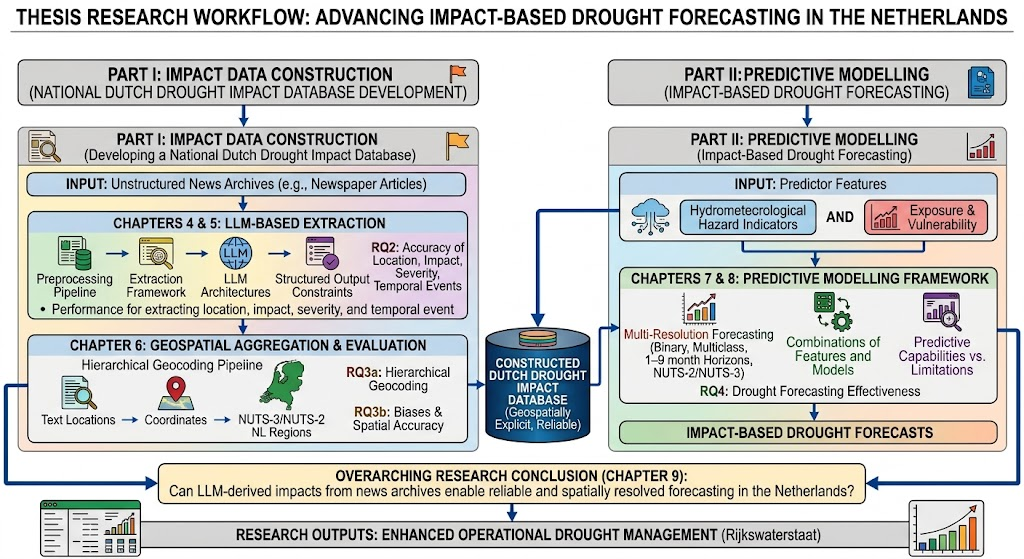
\includegraphics[width=1.05\linewidth]{figures/thesis researcworkflow.jpg}
    \caption{Overview of the research workflow, illustrating the connection between drought impact data construction, evaluation, and impact-based forecasting. [[ik moet de afbeelding nog updaten, staan wat fouten in zoals oude RQ]]}
    \label{fig:researchworkflow}
\end{figure}


The first research component investigates \textbf{(1)} \textit{What are the requirements of impacts of an drought impact dataset satisfy to support regional impact-based forecasting?} This chapter defines the problem and establishes the theoretical data requirements that guide the design of the drought impact database in Chapter~3.



Chapters~4 and~5 focus on the LLM-based extraction of drought impact events. Chapter~4 presents the overall methodology, including the preprocessing pipeline and extraction framework, while Chapter~5 evaluates the performance of different LLM architectures and structured extraction strategies. This component addresses the following research question: \textbf{(2)} \textit{How do different LLM architectures influence the performance of extracting location, impact, severity,
and temporal event information from unstructured text?} The key objective here is to get an reliability measure of our data, since LLMs tend to hallucinate.

Chapter~6 investigates the geospatial aggregation framework that transforms extracted textual information into spatially structured data suitable for predictive modelling. This framework consists of several components, including a point-based geocoding system that converts textual location references into geographic coordinates and an aggregation framework that maps these locations to administrative regions. This enables the extracted information to be represented as spatial features for machine learning applications. The corresponding research question is: \textbf{(3a)} \textit{How can a hierarchical geocoding pipeline be constructed to translate informal textual location references into NUTS-3 and NUTS-2 representations?} In the Netherlands, NUTS-2 regions correspond to the twelve provinces, while NUTS-3 regions represent smaller subregional administrative units. The objective of this aggregation framework is to generate spatial representations that allow machine learning models to identify regional patterns in drought impacts. Subsequently, the resulting database is evaluated to assess its spatial accuracy and reliability through the following research question: \textbf{(3b)} \textit{Which systematic biases, including regional reporting differences and environmental factors, affect the correspondence between news-derived impact data and reference datasets?}


Finally, Chapters~7 and~8 investigate the predictive modelling component of this thesis. This part addresses the following research question: \textbf{(4)} \textit{How effectively can the constructed drought impact database support impact-based drought forecasting in the Netherlands?} [@erik Will probably be changed to a baseline]

These chapters examine which combinations of predictor variables and modelling approaches provide the strongest predictive performance for drought impact forecasting. Model performance is evaluated across multiple spatial, temporal, and classification resolutions, including forecasting horizons ranging from one to nine months, predictions at both the NUTS-2 and NUTS-3 levels, and both binary and multi-class impact prediction tasks. The final chapter synthesises the findings from the preceding chapters and evaluates the broader implications of the proposed forecasting framework. In particular, it examines what the extracted information reveals about drought impacts in practice and discusses its potential contribution to operational drought management in the Netherlands.



% ==========================================
\chapter{Theoretical Background \& Literature}
% ==========================================

The goal of this chapter is to provide the theoretical background on Large Language Models (LLMs), information extraction, and impact-based drought forecasting. It reviews existing extraction methods, introduces the EDORA impact chain framework, summarizes current drought impact forecasting approaches, and discusses geoparsing techniques for extracting geospatial information from unstructured drought impact data.

\section{Theoretical Background of Large Language Models and Information Extraction}


\subsection{General Definition of Large Language Models}

Large Language Models (LLMs) are neural network-based models designed to learn statistical patterns in large collections of text. By modelling the probability distribution of sequences of tokens, LLMs can generate, transform, and extract information from natural language. In recent years, the application of LLMs has expanded rapidly, driven by advances in model architecture, computational resources, and large-scale training datasets.

The fundamental objective of an LLM is to predict the most likely next token given a preceding sequence of tokens. A token represents a discrete unit of text, such as a word or part of a word. Given an input sequence of tokens $x_1, x_2, ..., x_{t-1}$, the model estimates the probability distribution of the next token $x_t$:

\[
P(x_t \mid x_1, x_2, ..., x_{t-1})
\] During text generation, the next token can be selected based on this probability distribution, commonly by selecting the token with the highest estimated probability:

\[
x_t = \arg\max_x P(x \mid x_1, x_2, ..., x_{t-1})
\] Through this iterative process, LLMs generate coherent sequences of text based on the contextual information provided in the input. Modern LLMs are primarily based on the Transformer architecture introduced by Vaswani et al. \cite{vaswani2017attention}, which enables efficient processing of long text sequences and allows models to capture contextual relationships between tokens.

\subsection{Information Extraction with Large Language Models}

Information extraction (IE) refers to the transformation of unstructured text into structured representations, such as entities, attributes, and event-level records. Traditional IE approaches rely on supervised learning pipelines, including named entity recognition and relation extraction, which require manually annotated datasets and often generalise poorly beyond  training.

Large Language Models (LLMs) have shifted IE towards generative information extraction (GenIE), where extraction is formulated as structured generation guided by natural language instructions and output constraints \cite{gao2023llmsgenie}. Instead of requiring task-specific model training, LLMs can perform classification by adapting their behaviour through prompting and predefined output schemas \cite{gao2023llmsgenie}.

LLM-based extraction systems typically rely on several core mechanisms \cite{gao2023llmsgenie}. 
\textbf{(1) Generative information extraction}, where extraction tasks are reformulated as conditional text generation, allowing entities, relations, and events to be generated directly from input text using prompts and predefined schemas. 
\textbf{(2) Prompt design and structured generation}, where task instructions, demonstrations, and schema descriptions guide the model towards consistent extraction formats. 
\textbf{(3) Reasoning and refinement strategies}, where approaches such as chain-of-thought prompting, self-verification, or iterative refinement are explored to improve extraction accuracy and reduce errors \cite{gao2023llmsgenie}.

Despite these advances, ensuring that extracted information is both structurally valid and faithful to the source text remains a key challenge. LLMs may generate plausible but incorrect information, commonly referred to as hallucinations. Therefore, validation procedures and reliability assessments remain essential when applying LLM-based extraction methods for scientific dataset construction.


\section{Drought Risk Framework: Impact Chain Theory}


Impact Chain Theory provides a structured framework for analysing climate-related risks by explicitly representing the relationships between hazard, exposure, vulnerability, and resulting impacts. Within this framework, risk is understood as the outcome of interacting system components rather than as a direct consequence of hazard conditions alone.

The European Drought Risk Atlas (EDORA) operationalises this approach through the construction of sector-specific impact chains, developed through a combination of literature review and expert consultation \cite{EDORA}. These impact chains describe sequences of processes linking hydrometeorological conditions to sectoral consequences. For instance, elevated temperatures and precipitation deficits may lead to soil moisture depletion, reduced crop productivity, and increased irrigation demand. Individual elements within these chains are categorised according to hazard, exposure, vulnerability, and impact.

To enable quantitative analysis, EDORA represents these conceptual relationships using proxy variables. Hazard indicators are derived from hydro-meteorological data, while drought impact indicators are obtained from datasets such as EDID (European Drought Impact Database). Vulnerability and exposure are approximated using socio-economic and environmental variables, including land use, economic activity, and climatic characteristics. These components are combined to estimate sectoral drought risk \cite{EDORA}. For example, EDORA uses impact chain theory to estimate the sectoral risk of wheat yield reduction. 

The resulting framework provides a formal representation in which drought impacts arise from the interaction between hazard conditions, exposed systems, and their underlying vulnerabilities. This relationship can be expressed in general functional form as:

\[
\text{I} = f(H, E, V)
\]

where $H$ denotes hazard conditions, $E$ represents exposure, and $V$ captures vulnerability. The function $f()$ describes how these components jointly determine the observed impacts, $I$.

In this thesis, the impact chain framework serves as the conceptual foundation for defining the machine learning input space. The relationship between hazard indicators and observed impacts is approximated using data-driven modelling techniques. This formulation allows the incorporation of heterogeneous data sources, including impact information derived from unstructured textual data. Examples of data that fit within this impact chain framework include meteorological, hydrological, and agricultural indices for hazard indicators. For exposure indicators, land-use ratios are primarily considered. For vulnerability, population density within a region (PopR) is used as an indicator.

\label{sec:impact_chain_theory}







\section{Impact-Based Drought Forecasting: Concept and Literature}
\label{sec:ibf_literature}
\subsection{Definition of Impact-Based Drought Forecasting}

Impact-based forecasting (IbF) predicts the expected consequences of drought for socio-economic and environmental systems, rather than drought conditions alone \cite{WMO2021, PrevenionWeb2022, Shyrokaya2024Advances}. Instead of relying solely on hazard indicators such as the Standardized Precipitation Index (SPI) or the Standardized Precipitation Evapotranspiration Index (SPEI), it relates meteorological and hydrological conditions to observed impacts, such as agricultural losses, reduced crop yields, wildfire risk, and water shortages \cite{Sutanto2019Moving, Bulut2026Framework}.

By incorporating exposure and vulnerability alongside drought hazard indicators, impact-based forecasting supports early warning and decision-making across sectors including agriculture, water management, ecosystems, and infrastructure \cite{WMO2021, Shyrokaya2024Advances}.



\subsection{Modelling Approaches in Impact-Based Drought Forecasting}

Existing studies commonly estimate relationships between drought indicators and observed impacts using statistical or machine learning methods. Logistic regression, generalized additive models, Random Forests, and gradient boosting approaches are among the most frequently applied techniques \cite{Stagge2015Modeling, Bachmair2017Developing, Sutanto2019Moving, Bulut2026Framework}. 

Many of these approaches use hydro-meteorological variables such as precipitation deficits, soil moisture anomalies, river discharge, or evapotranspiration as predictive features. In several studies, machine learning methods have demonstrated improved capability in capturing nonlinear relationships between drought conditions and reported impacts \cite{Sutanto2019Moving, Bulut2026Framework}. Tree-based methods are frequently identified as effective under conditions of sparse or noisy impact data due to their flexibility and relatively limited assumptions regarding variable distributions.

The majority of impact-based drought forecasting studies rely on existing impact inventories, most notably the European Drought Impact report Inventory (EDII). These datasets are typically combined with meteorological observations or reanalysis products in order to model the probability, severity, or occurrence of drought impacts across sectors and regions.

\subsection{Spatial and Temporal Scales}

The spatial scale of impact-based drought forecasting is strongly influenced by the structure of available impact datasets. Most studies operate at aggregated administrative levels, including NUTS-2 regions (provinces) or NUTS-1 regions (e.g., western Netherlands), because impact observations are rarely available at finer spatial resolutions \cite{Sutanto2019Moving, Bulut2026Framework, Shyrokaya2024Advances}.

Forecast horizons also vary substantially across studies. Short lead times (0 to 3 months) generally achieve higher predictive skill, whereas longer lead times require broader accumulation periods or additional proxy variables to maintain performance \cite{Sutanto2019Moving, Shyrokaya2025HowGood}. Note that the results reported by Sutanto ~\cite{Sutanto2019Moving} may be affected by data leakage, potentially leading to overly optimistic performance estimates.

The Critical Threshold for prediction seems to be around 6 months, where skill often becomes equivalent to random guessing \cite{Bulut2026Framework}. 


% \subsection{Current Limitations}

% Despite methodological advances, current impact-based drought forecasting systems remain constrained by the availability and structure of impact data. Existing datasets often exhibit limited spatial precision, inconsistent reporting standards, and uneven sectoral representation \cite{Shyrokaya2024Advances, Bulut2026Framework}. These limitations reduce the reliability and transferability of predictive models and restrict the level of spatial and semantic detail that can be represented within operational forecasting systems.

\subsection{Current Limitations}

Despite methodological advances, current impact-based drought forecasting systems remain constrained by the availability and structure of impact data. Existing datasets often exhibit limited spatial precision, inconsistent reporting standards, and uneven sectoral representation \cite{Shyrokaya2024Advances, Bulut2026Framework}. For example, text-based impact datasets commonly rely on administrative (NUTS) geocoding, where reported impacts are assigned to regional centroids rather than their exact locations, limiting their suitability for fine-scale analysis \cite{sodoge2023}. Furthermore, impact records often lack consistent temporal information, with some reports only providing seasonal or annual descriptions rather than precise occurrence dates \cite{Bulut2026Framework, Sutanto2019Moving}. Existing datasets are also frequently biased towards well-documented sectors, such as agriculture, while impacts in sectors with less standardized reporting remain under-represented \cite{Shyrokaya2024Advances}.



\section{Text-Based Extraction of Geospatial Drought Impact Information}
\label{sec:text_extraction}
\subsection{Geoparsing and Named Entity Recognition}

The extraction of geographic information from textual sources commonly relies on geoparsing pipelines that combine named entity recognition (NER) with geocoding techniques \cite{Gritta2018, Karimzadeh2019Geoparsing}. Within environmental and disaster-related applications, these approaches are frequently used to identify locations associated with reported impacts in news articles, reports, or social media content.

Most geoparsing systems first detect location mentions using NER models and subsequently map these entities to geographic coordinates or administrative regions through gazetteers such as GeoNames \cite{Gritta2018}. Traditional approaches often employ rule-based systems or statistical NLP models, while more recent methods increasingly rely on transformer-based architectures for contextual entity recognition and disambiguation.

In drought impact research, Sodoge et al.~\cite{sodoge2023} combine spaCy-based NER with GeoNames matching and hierarchical clustering to identify affected regions from textual sources. Their method achieves high alignment accuracy between extracted clusters and article scope. SeqIA~\cite{lopez2025} adopts a transformer-based approach using RoBERTa for location recognition together with dependency parsing to resolve ambiguous place names.

Although these approaches improve the extraction of geographic information, they remain constrained by document-level assumptions and limited spatial representation. Many geoparsing pipelines implicitly assume a single dominant impact location per document, reducing their ability to represent spatially distributed drought impacts across multiple regions.

\subsection{Drought Impact Extraction}

Alongside geographic information extraction, recent studies have increasingly focused on identifying and categorising drought impacts directly from textual data. This task generally involves classifying text fragments into predefined impact categories such as agriculture, forestry, water supply, or wildfires.

Earlier approaches relied primarily on conventional machine learning methods using manually engineered textual features. Sodoge et al.~\cite{sodoge2023}, for example, apply lasso-regularised logistic regression on tf-idf representations, reporting high classification performance across several drought impact categories.

More recent systems employ transformer-based language models for relevance detection and impact classification. SeqIA~\cite{lopez2025} combines Longformer architectures with RoBERTa classifiers to identify drought-related content and assign impact categories using supervised learning approaches.

% Compared to location extraction, impact-type classification generally exhibits stronger and more stable performance across studies. This is partly due to clearer semantic distinctions between impact categories and the availability of annotated training datasets.

\subsection{Large Language Models for Information Extraction in climate research}

The emergence of large language models (LLMs) has created new opportunities for information extraction in geospatial and environmental applications. Unlike traditional supervised NLP systems, LLMs can perform zero-shot (no train samples) or few-shot extraction without requiring large labelled datasets.

Recent work has applied prompt-based LLMs to drought impact extraction. For example, CienaLLM~\cite{ciena2025} extracts drought impacts and affected administrative regions from Spanish news articles, achieving competitive impact classification while highlighting remaining challenges in location extraction.

Compared to traditional pipeline-based approaches, LLMs can jointly extract locations, impact descriptions, severity indicators, and temporal references within a single inference process, enabling more flexible representations of drought impacts.



% \subsection{Current Limitations}

% Despite recent advances, the extraction of high-resolution drought impact information from textual sources remains limited by several structural challenges. Existing methods often struggle to represent multiple geographically distributed impacts within a single document. 

% The reliability of extracted datasets is also affected by inconsistencies in reporting practices, linguistic ambiguity, and uneven spatial coverage in news sources. These limitations constrain the construction of structured drought impact datasets suitable for predictive modelling and operational forecasting applications \cite{sodoge2023, lopez2025, ciena2025}.








%\section{The Dutch Hydrological and Socio-Economic Context} later;depends on steak holder


% ==========================================
\chapter{Problem Definition \& System Requirements}
\label{ch:problem_definition}

In this chapter we define the problem and establishes the theoretical data requirements that guide the design of the drought impact database. \textit{What are the requirements of impacts of an drought impact dataset satisfy to support regional impact-based forecasting?} 

% ==========================================
\section{Defining the Data and Modelling Gap in Drought Impact Research}

% \subsection{Data limitations for impact-based drought forecasting}

% The literature reviewed in Chapter~2 shows that a key challenge in impact-based drought forecasting is not only the development of predictive models, but also the availability of suitable impact datasets. Machine learning models require impact observations that are consistent in terms of location, timing, and impact type. However, existing drought impact datasets often have limited spatial detail (nuts-1 instead of nuts3), and a relatively small number of observations only 268 for nl.

% Existing drought impact inventories, such as the European Drought Impact Inventory (EDII), provide valuable information on observed drought impacts and have supported previous impact-based forecasting studies. However, these inventories were mainly developed for documenting and analysing drought events rather than for creating large-scale datasets for machine learning applications. As a result, studies using these datasets often combine impacts into broad categories or aggregate observations over larger regions to obtain sufficient data for modelling \cite{Sutanto2019Moving, Blauhut2015Towards}. Although this improves model development, it reduces the ability to predict specific impacts at local scales .

% Creating impact-based forecasting systems requires a balance between data quality, spatial detail, temporal coverage, and the number of available observations. Curated impact inventories generally provide reliable observations but contain a limited number of records. Newspaper articles, in contrast, provide a much larger source of historical information and often contain detailed descriptions of local drought impacts. However, they also contain uncertainties caused by reporting bias, inconsistent terminology, and incomplete descriptions.

% This thesis investigates whether newspaper-based impact information can complement existing drought impact inventories by providing a larger and more spatially detailed dataset for machine learning applications. The aim is not to replace existing databases, but to develop a scalable approach for extracting additional impact observations. Using large language models (LLMs), newspaper articles are transformed into structured impact-location records, allowing individual impacts to be linked to their reported locations.

% The resulting dataset provides additional information on drought impacts over longer time periods and across more locations. However, newspaper-based observations remain affected by limitations such as uneven reporting between sectors, differences in media attention, and uncertainty in impact severity. These limitations are considered when evaluating the suitability of the dataset for impact-based drought forecasting.


\subsection{Data limitations for impact-based drought forecasting}

The literature reviewed in Chapter~2 shows that a key limitation in impact-based drought forecasting is the availability of suitable impact datasets. While existing inventories such as the European Drought Impact Inventory (EDII) provide valuable information on observed drought impacts, they were primarily developed for documenting and analysing drought events rather than for creating large-scale datasets for machine learning applications.

Consequently, current forecasting studies are often limited by the number of available observations, coarse spatial resolution, and inconsistent impact descriptions. For example, EDII-based studies commonly aggregate impacts over larger administrative regions [NUTS-1] or broader impact categories to obtain sufficient data for modelling \cite{Sutanto2019Moving, Blauhut2015Towards}. Although this enables forecasting, it reduces the ability to predict specific impacts at local scales.

This creates a need for impact datasets that provide a larger number of observations while maintaining detailed spatial and impact information. Newspaper articles offer a complementary data source by providing a long historical record of locally reported drought impacts. However, these sources introduce uncertainties related to reporting bias, inconsistent terminology, and incomplete descriptions.

Therefore, this thesis investigates whether large-scale extraction of newspaper-based drought impact information using large language models (LLMs) can be used to construct a Dutch drought impact database. The objective is to develop a scalable approach for generating spatially detailed impact-location records that can support the development of impact-based drought forecasting models in the Netherlands.


\section{Drought Impact Requirements for Impact-Based Forecasting}
The previous section highlighted the need for a Dutch drought impact database suitable for impact-based forecasting. However, constructing such a database requires careful consideration of the information needed by predictive models. This section defines the requirements for the drought impacts extracted from newspaper articles. The structure of the dataset determines the spatial detail, impact specificity, and temporal information available for forecasting. Therefore, the database developed in this thesis is designed around four key requirements: spatial resolution, impact categorisation, temporal representation, and explicit impact-location relationships.

\subsection{Spatial Resolution (NUTS-2 / NUTS-3)}

Spatial resolution is a key requirement for impact-based drought forecasting. Existing studies often operate at aggregated administrative scales because impact observations are rarely available at finer spatial levels. However, this limits the ability to capture regional differences in drought impacts.

The database developed in this thesis aims to preserve point-level impact information and provide spatial information at NUTS-2 and NUTS-3 levels. This resolution provides a balance between spatial detail, data availability, and compatibility with meteorological, hydrological, and socio-economic datasets used for forecasting.

\subsection{Impact Categorisation and Severity Information}

Impact-based drought forecasting requires information on the specific consequences of drought rather than drought conditions alone. However, existing impact datasets often combine multiple impacts into broad categories to compensate for limited observations. While this increases the number of available samples, it reduces the detail and interpretability of predicted impacts.

The database developed in this thesis aims to preserve sector-specific impact information during extraction. This includes categories such as agriculture, ecology, forestry, navigation, water supply, and infrastructure-related impacts. Maintaining detailed categories during database construction provides flexibility during later modelling stages, where categories can be combined if required.

The database also aims to capture impact severity information where available. Distinguishing between minor disruptions and severe impacts provides additional information for predictive modelling.

\subsection{Temporal Representation}

Drought impacts often occur with a delay after changes in meteorological conditions. Agricultural losses, ecological impacts, groundwater depletion, and economic disruptions may develop weeks or months after drought onset. Furthermore, newspaper articles are not always published at the time an impact occurs, meaning publication date does not necessarily represent impact timing.

Therefore, the database should capture temporal information beyond article publication date where possible. This enables a better representation of the relationship between drought conditions and observed impacts, which is important for forecasting models using different lead times.

\subsection{Multi-Location Impact Extraction}

A limitation of many conventional geoparsing approaches is that they often assume a document contains one dominant location. However, drought-related articles frequently describe multiple impacts occurring across different regions. When locations are extracted only at the document level, the relationship between individual impacts and their associated locations can be lost.

The extraction framework developed in this thesis therefore focuses on identifying explicit impact-location relationships. Instead of assigning a single location to an entire document, individual impact descriptions are linked to their corresponding geographic regions. This increases the spatial detail of the resulting database and improves its suitability for regional impact-based drought forecasting.


% ==========================================
\part{Impact Data Construction and Validation}
\label{part A}
% ==========================================

\chapter{Drought Impact Database Construction Framework}
\label{ch:llm_pipeline}

\section{Drought Impact Database Construction Framework}
The construction of the drought impact database consists of five main stages: data collection, preprocessing, LLM-based information extraction, geospatial processing and aggregation, and validation. Together, these stages transform unstructured newspaper articles into a structured and spatially explicit drought impact database.

This chapter introduces the data collection process, preprocessing steps, and the LLM-based extraction framework. The extraction framework is subsequently evaluated to identify the most suitable model configuration. The extracted impact records are then geocoded, aggregated to NUTS-2 and NUTS-3 regions, and validated using external data sources to assess the quality of the resulting database.

Figure~\ref{fig:pipeline_overview} provides an overview of the complete database construction framework and the corresponding chapters in Part~I.


\begin{figure}[h]
    \centering
    \fbox{
        \parbox{0.96\textwidth}{
        \centering

        \textbf{Input}\\[0.15cm]
        Newspaper Articles

        \vspace{0.3cm}
        $\downarrow$
        \vspace{0.3cm}

        Data Collection
        $\rightarrow$
        Preprocessing
        $\rightarrow$
        Extraction Framework\\
        \small (Chapter~4)

        \vspace{0.3cm}
        $\downarrow$
        \vspace{0.3cm}

        Extraction Performance \& Configuration Selection\\
        \small (Chapter~5)

        \vspace{0.3cm}
        $\downarrow$
        \vspace{0.3cm}

        Geospatial Processing \& Aggregation
        $\rightarrow$
        Visualization \& Validation\\
        \small (Chapter~6)

        \vspace{0.3cm}
        $\downarrow$
        \vspace{0.3cm}

        \textbf{Output}\\[0.15cm]
        Dutch Drought Impact Database
        }
    }
    \caption{Overview of the drought impact database construction framework and the corresponding chapters in Part~I.}
    \label{fig:pipeline_overview}
\end{figure}


% The construction of a drought impact database requires transforming unstructured information sources into structured and spatially explicit impact records. This chapter presents the framework developed to construct the drought impact database used throughout Part~I of this thesis. The workflow consists of five main stages: data collection, preprocessing, LLM-based information extraction, geospatial processing and aggregation, and validation.

% The workflow begins with data collection, where relevant newspaper articles are gathered using a semi-automated approach. These articles are subsequently processed through several preprocessing steps to remove irrelevant information, reduce redundancy, and prepare the text for automated extraction.

% Following preprocessing, large language models (LLMs) are used to extract structured drought impact information from the articles. Chapter~\ref{ch:extraction_performance} investigates how different LLM configurations and structured output constraints influence extraction performance. Selecting an appropriate extraction configuration is challenging because drought impacts described in text can have multiple valid interpretations, requiring evaluation against human judgement.

% After extraction, the identified impact records undergo geospatial processing, where extracted locations are converted into geographic coordinates and aggregated to NUTS-2 and NUTS-3 regions. This step creates a spatially consistent dataset suitable for further analysis and forecasting applications in part II. Finally, the resulting database is analysed through a visualization framework and evaluated using external data sources to assess extraction quality and identify remaining uncertainties.

% The final outcome of this workflow is a structured drought impact database containing spatially explicit impact records, together with an assessment of its quality and limitations.


% \begin{figure}[h]
%     \centering
%     \fbox{
%         \parbox{0.9\textwidth}{
%         \centering
%         Newspaper Articles 
%         $\rightarrow$
%         Data Collection 
%         $\rightarrow$
%         Preprocessing 
%         $\rightarrow$
%         LLM-based Extraction 
%         $\rightarrow$
%         Geospatial Processing \& Aggregation 
%         $\rightarrow$
%         Visualization \& Validation
%         }
%     }
%     \caption{Overview of the drought impact database construction framework. The framework transforms unstructured newspaper articles into structured and spatially explicit drought impact records.}
%     \label{fig:pipeline_overview}
% \end{figure}










% %1. preprecossing
% %2. extraction
% %2. Geocoding
% %4. visuliazation and validaiton

% The 








% \begin{figure}[h]
%     \centering
%     \fbox{
%         \parbox{0.9\textwidth}{
%         \centering
%         Preprocessing $\rightarrow$ LLM extraction $\rightarrow$ Geocoding $\rightarrow$ Visualisation  $\rightarrow$ 
%         Validation
        
%         }
%     }
%     \caption{High-level overview of the drought impact extraction pipeline}
%     \label{fig:pipeline_overview}
% \end{figure}


% To construct and get our drought impact database, several steps have been taken to get to the final results. First we have to collect the right data, this has been been done in the data collection step, wich was done using an semi-automation. Then after that we applied several preporcceing techniche's, to clean the data and make it machine ready. In chapter 5 we further explore llmn configuration settings, and pick an model that works the best for use case, based on human validation. This is not an trivilial task, becauce, one event might have multiple correct anwsers. After Evaluating the best peformance setup, we geoceode the data, and create an aggregation framework, to aggereate our data into nuts3 regoin. WHne that is done we feed the data through an visulization tool, and peform validation studies, using external data sources. This leaves us with an dataset where reliabilty has sort of been estimated towards succes. 







% The proposed system consists of a modular pipeline that transforms unstructured news articles into a structured and geospatially explicit dataset of drought impacts. This system architecture is the core of Part \hyperref[part A]{I}. In the current chapter, we focus on the preprocessing step and the LLM-based extraction framework. While Chapter \ref{ch:extraction_performance} is focused on the Extraction Performance and Configuration Selection. Chapter \ref{ch:geocoding}, we evaluate the final 3-steps of the pipeline Geocoding, visualization and validation.

% This architecture integrates multiple processing stages, including preprocessing, large language model-based information extraction, geocoding, and visualisation, as illustrated in Figure~\ref{fig:pipeline_overview}.

% The pipeline begins with data entry and extraction, followed by preprocessing steps that include cleaning, deduplication, and basic feature extraction (see Section \ref{ch:preprocessing}). The processed text is then passed to a large language model, which identifies and structures drought-related impact information from unstructured articles (see Section \ref{Extraction Framework Design}).

% Extracted location mentions are subsequently transformed into geospatial coordinates through a geocoding step, enabling spatial interpretation of impact events. The resulting structured dataset is exported for downstream analysis (see Section \ref{nuts_coding}).

% A Streamlit-based interface is used for visualisation of geocoded impacts and supports exploratory analysis as well as validation of extracted results (see Section \ref{vis}).


\newpage
\section{Data Acquisition: News Archives and Pre-processing}
In this section, a synthetic sample of a news article is presented to illustrate the type of data used in this study. Subsequently, the data acquisition and preprocessing steps are described.

\subsection{A Single News Article}

Newspaper articles contain valuable information about drought impacts that can be extracted and transformed into structured records. News articles often contain relevant details such as the affected sector, impact type, location, and temporal information. The following example illustrates the type of information that can potentially be extracted from newspaper articles for the construction of a drought impact database.

\begin{framed}
\footnotesize
\textbf{Publicatiedatum:} 15 augustus 2018

\medskip

\textbf{Droogte zorgt voor lagere aardappelopbrengsten in Zeeland}

De aanhoudende droogte van de zomer van 2018 heeft grote gevolgen voor aardappeltelers in Zeeland. Door het langdurige neerslagtekort en de droge bodem hebben verschillende boeren te maken met lagere opbrengsten dan normaal.

Volgens lokale landbouwers hebben aardappelplanten door het watertekort kleinere knollen ontwikkeld. Om verdere schade te beperken, hebben veel boeren extra beregend, maar door de beperkte beschikbaarheid van water werd dit steeds moeilijker.
\end{framed}

From this article, several features can potentially be extracted, including the publication date, location (Zeeland), affected sector (agriculture), and impact type (crop yield reduction). Note that, when reading the article closely, additional impacts can also be identified, such as water limitations caused by drought conditions.

These extracted features can subsequently be structured into a drought impact record and linked to geographic information.






\subsection{Automated Data Acquisition and Preprocessing}
\label{ch:preprocessing}

\begin{figure}[h!]
    \centering
    \fbox{
    \begin{minipage}{0.95\textwidth}
    \centering
    \small
    \setlength{\jot}{2pt}
    \begin{aligned}
        \text{LexisNexis Archive}
        &\rightarrow \text{Playwright-based Scraping}
        \rightarrow \text{Deduplication (MinHash + LSH)} \\
        &\rightarrow \text{Text Cleaning \& Feature Extraction}
        \rightarrow \text{Temporal Annotation}\\
        \rightarrow \text{LLM-ready Corpus}
    \end{aligned}
    \end{minipage}
    }
    \caption{Preprocessing pipeline transforming raw news archives into a structured corpus for downstream LLM extraction.}
    \label{fig:preprocessing_pipeline}
\end{figure}

The dataset is sourced from LexisNexis Nexis Uni, accessed through an institutional subscription. The platform imposes strict retrieval constraints, including a daily download limit of approximately 1,500 news articles and restricted pagination functionality. These limitations significantly reduced the download speed, resulting in an estimated collection period of more than 100 days. To facilitate this incremental daily data collection, an automated scraping pipeline was developed to enable systematic data retrieval.

The overall preprocessing workflow is summarised in Figure~\ref{fig:preprocessing_pipeline}. A Playwright-based scraping framework is used to interact with the platform. The system simulates user interaction by navigating search results, selecting article batches, and initiating downloads through the web interface. The search query was constructed to maximise coverage of drought-related content across domains such as agriculture, water resources, forestry, infrastructure, and public health [ADD queery to appenidx].

The resulting dataset contains redundancy due to repeated reporting of the exact same news articles. To address this, all retrieved articles are subjected to global deduplication. Near-duplicate detection is performed using a MinHash and Locality-Sensitive Hashing (LSH) framework, which removes redundant entries while preserving semantically distinct articles. Note that no additional steps were not taken to remove semantically similar news articles.


After deduplication, structured feature extraction is applied. Article-level metadata, including title, source identifier, and publication date, is extracted using rule-based regular expressions. The article body is cleaned by removing headers, metadata blocks, and non-content segments based on predefined markers.

The article body cleaning procedure is evaluated using a cleaning ratio, defined as the proportion between original and cleaned text length. Articles with extreme values in this metric are excluded based on a distribution-informed threshold approach. Further more we manually check for suspicious cases.

Finally, publication dates are reintroduced into the cleaned text to preserve temporal context for downstream large language model processing. 
\section{LLM Extraction Framework}


This section describes the design of the LLM-based extraction framework. First, the system prompt and Pydantic schema used to structure the LLM output are introduced. Afterwards, the extracted variables and their representation within the drought impact event structure are described.

\label{Extraction Framework Design}


\subsection{System Prompt Design}
A system prompt was developed to guide the LLM-based extraction of structured drought impact events from newspaper articles. The system prompt, together with the Pydantic schema, is sent through an API to an LLM provider. The system prompt defines the general extraction task and provides the instructions that guide how the model should populate the structured output.

The system prompt contains several components. First, it defines the available impact categories from which the model can select. Second, it provides additional field guidance describing how the individual fields in the Pydantic schema should be completed. Although some of this information is also encoded directly in the Pydantic schema, it is repeated in the system prompt to improve consistency and reduce extraction errors.

The field guidance specifies how the model should extract locations, estimate recency, and identify drought impacts. It also includes a reasoning field, where the model explains why a location and associated impacts are derived from the article text. Additionally, the prompt defines seven critical rules that constrain the extraction process. The most important rule is that only realized drought consequences explicitly supported by the article should be extracted. This prevents the model from including speculative impacts, future adaptation measures, or general drought-related statements without a reported impact.

The complete system prompt is provided in Appendix~\ref{...}.

\subsection{Extraction Schema}

The extraction schema defines the structure of the LLM output and is implemented using the Python library Pydantic. Pydantic was selected because it supports schema-based output constraints across multiple LLM API providers. The schema forces the model output into a predefined JSON structure and enables automatic validation of extracted records.

After extraction, the generated output is validated within the processing pipeline. If the response cannot be parsed according to the predefined schema, the extraction request is repeated. This ensures that all extracted records follow a consistent structure before further processing.

The initial extraction schema represented each article as a collection of independent events. An event was defined as a unique combination of a location and a sentence-level fact. Each event contained a single impact label, severity or recency value, and evidence span. This structure was later revised to better represent the multi-label nature of drought impacts.



\subsection{Drought Impact Category Selection}

The first step in designing the extraction framework was determining which drought impact variables should be extracted from newspaper articles. To guide this process, a literature review on impact-based drought forecasting was conducted. Rather than developing a new categorisation from scratch, the initial framework was based on the impact categories most commonly used in previous studies.

Although the exact definitions differ between impact based forecasting studies, most organise drought impacts into four to eight broad categories. The most common groups are Agriculture and Livestock Farming, Energy and Industry, Public Water Supply, Water Resources and Water Quality, Ecosystems, and Wildfires. Many studies further aggregate these into four broad sectors: agriculture, energy, water supply, and water resources \cite{Stagge2015Modeling, lopez2025, Bulut2026Framework}. Other studies, additionally distinguish forestry, wildfires, and human health impacts \cite{Sutanto2019Moving, sodoge2023}. Although many studies adopt the 15 categories defined by the European Drought Impact Inventory (EDII), these are often aggregated into broader groups for modelling purposes.

Rather than using these broad categories, this thesis adopts a more detailed taxonomy consisting of 20 impact categories (Table~\ref{tab:impact_categories}). Because extraction is performed using zero-shot classification, the LLM is not limited by predefined training labels. A finer taxonomy therefore allows related impacts to be extracted separately, such as distinguishing Thermal/Nuclear Cooling Constraints from Industrial Water Shortages, or Forest Dieback from Wetland Loss. These detailed categories can later be aggregated into broader groups when required for forecasting or analysis.

\begin{table}[htbp]
\centering
\caption{Drought impact categories used in the extraction framework.}
\label{tab:impact_categories}
\footnotesize
\setlength{\tabcolsep}{3pt}
\renewcommand{\arraystretch}{1.0}
\begin{tabular}{lll}
\hline
Crop Failure \& Yield Reduction &
Hydropower Reduction &
Wildfire Occurrence \\
Livestock Stress \& Mortality &
Thermal/Nuclear Cooling Constraints &
Wildfire Risk Increase \\
Irrigation Shortage &
Industrial Water Shortages &
Heat \& Air Quality Health Impacts \\
Groundwater Depletion &
Inland Waterway Disruption &
Water Supply \& Sanitation Issues \\
Reservoir \& Surface Water Shortage &
Freshwater Ecosystem Degradation &
Agricultural Economic Loss \\
Water Use Restrictions &
Forest Dieback \& Vegetation Stress &
Broader Economic Disruption \\
&& Social Impacts \\
\hline
\end{tabular}
\end{table}


\newpage
\subsection{Event Representation}

The LLM extraction framework converts unstructured newspaper articles into structured drought impact events. Each event represents a reported drought impact linked to a specific location. An overview of the extracted event structure is provided in Table~\ref{tab:feature_schema_overview}. The following subsections describe the design choices behind each component in more detail.

\begin{table}[h!]
\centering
\renewcommand{\arraystretch}{1.2}
\begin{tabular}{ll}
\toprule
\textbf{Feature} & \textbf{Representation} \\
\midrule
Location & Geographic entity mentioned in the article text \\
Impact class & One or more labels from a 20-category drought impact taxonomy \\
Severity & Ordinal impact magnitude score (1--3) \\
Recency & Time since impact relative to publication date \\
Evidence & Verbatim text span supporting the extracted impact \\
Reasoning & Explanation of the location and impact extraction \\
Event structure & One event per location with associated impact categories \\
\bottomrule
\end{tabular}
\caption{Core variables in the LLM-based drought impact extraction schema.}
\label{tab:feature_schema_overview}
\end{table}
\subsubsection{Realised versus Predicted Drought Impacts}

The extraction framework focuses on realized drought impacts rather than expected consequences or adaptation measures of an drought. The objective is to ensure that the database contains observed drought impacts rather than potential future impacts.


\subsubsection{Multi-event and Multi-location Extraction}

A single article can describe drought impacts across multiple locations and sectors. To preserve spatial detail, the framework represents each distinct location mentioned in an article as a separate event, with one or more associated impact categories.

For example, an article stating that "farmers in Zeeland experienced irrigation shortages, while forests in Brabant showed signs of drought-related vegetation stress" would result in two separate events: one event linked to Zeeland with an irrigation shortage impact, and one event linked to Brabant with a forest vegetation stress impact. This differs from many traditional extraction approaches, where an article is often assigned a single dominant impact category. The proposed framework can therefore capture multiple impacts from a single sentence. Locations are extracted exactly as they are mentioned in the original text to preserve the information provided by the article.


\subsubsection{Controlled Impact Classification}

Extracted impacts are restricted to a predefined taxonomy of 20 drought impact categories (Table~\ref{tab:impact_categories}). This improves consistency and allows detailed classification of drought impacts while maintaining the possibility of later aggregation into broader impact groups.


\subsubsection{Temporal Recency Estimation}

The LLM is instructed to estimate recency based on temporal information provided within the article itself. For example, an article may state that an impact occurred "three months ago" or "last month". These references are converted into predefined recency values, providing additional temporal information for downstream impact forecasting. The main objective is to improve the predictive signal, as newspaper articles may describe impacts after they have already occurred, creating a temporal lag between the event and its reporting.


\subsubsection{Severity Assessment}

Each impact is assigned a severity score from 1 to 3 based on the reported extent and consequences of the impact. The severity guidance is adapted from the European Drought Impact Database, where 1 represents low/minor impacts, 2 represents medium/moderate impacts, and 3 represents high/extreme impacts. This provides an additional measure of impact magnitude for forecasting applications.


\subsubsection{Evidence Extraction and Reasoning}

Each event contains an evidence quote and reasoning field to improve transparency and enable manual validation of extracted impacts. The evidence quote provides the specific text supporting the extraction, for example: "Due to prolonged drought, farmers in Brabant were unable to irrigate their crops, resulting in significant yield losses."








% For our extraction schema, we use an library called pydantic, the reason we specfiiclay hcoose dfor pydatnic, for schema based output constraines is that is supported multiple llm api providers . The idea beheind an extraction schema is that the llmn is forced to output the text into schema. If it doesn't happen the llmn checks internally if it did  do that or not. Next to it after the extracition, we check in our code if the schema was pasred correclty, if not we resend the prompt to the llmn provider. The extraction schema design and the way we extracted variable's, was changed during the thesis because we thoaught anothe schema would incrasse peformacen. First our orignal extraction schema design strucutre was We have an article, we define an event as a nunique location + an fact of sentence level, then for each event we have a single impact lable and a nsingle severity or recency label, with an eivdneance span. 

% So an event o address these limitations, we introduce a post-hoc evaluation method. We sample ten manually
% verified relevant articles and evaluate model outputs in terms of false positives and false negatives at the
% extraction level. This allows us to approximate fuzzy set membership directly from predictions without
% enforcing rigid categorical boundaries.
% In parallel, we revise the model output structure to better reflect the multi-label nature of the task.
% Instead of allowing an unbounded number of extracted tuples, we enforce a hierarchical event represen-
% tation.
% The original structure was:
% • Article → Event (location + sentence-level fact)
% • Single impact label
% • Single severity or recency label
% • Single evidence span
% This is replaced by a structured formulation















% The extraction framework converts unstructured news articles into structured drought impact events while satisfying the requirements from Section 3.2, including NUTS-2/3 spatial resolution, impact categorization, severity estimation, temporal recency, and multi-location extraction.










% %0. What are the varialble's we need to extract.

% %1. How do we extract it.

% %1. What extracation framewrok we used

% %2. What is our system prompt

% %3. What is the pydantic strucutre we used
% The extraction framework converts unstructured news articles into structured drought impact events while satisfying the requirements from Section 3.2, including NUTS-2/3 spatial resolution, impact categorization, severity estimation, temporal recency, and multi-location extraction.



% An overview of the resulting event representation is provided in Table~\ref{tab:feature_schema_overview}. The framework is operationalised through a structured JSON schema enforced via Pydantic, combined with prompt-level constraints that ensure consistent extraction of all event attributes.
% \begin{table}[h!]
% \centering
% \renewcommand{\arraystretch}{1.2}
% \begin{tabular}{ll}
% \toprule
% \textbf{Feature} & \textbf{Representation} \\
% \midrule
% Location & Named geographic entity (free text, geoparsed to NUTS-2/3) \\
% Impact class & Constrained label set (20 categories) \\
% Severity & Ordinal scale (1--3) \\
% Recency & Discrete temporal buckets (0, 1, 2--24 months) \\
% Evidence & Verbatim quote (max 25 words) \\
% Reasoning & Free-text justification of classification \\
% Event structure & One record per location--impact pair \\
% \bottomrule
% \end{tabular}
% \caption{Core variables in the LLM-based drought impact extraction schema.}
% \label{tab:feature_schema_overview}
% \end{table}

% \subsection{Realised versus Predicted Drought Impacts}

% One design objective is to ensure that forecasts are non-speculative or future-oriented. News articles often include forecasts or warnings that do not correspond to observed consequences. An IBF model has no need for such impacts. To reduce the number of false positives originating from these kinds of articles, we enforce the following instruction.

% This is enforced through instructions such as:

% \begin{quote}
% ``Only include real consequences of drought; avoid vague inferences.''
% \end{quote}

% The reasoning field requires explicit justification of whether an impact is observed:

% \begin{quote}
% ``First, identify if the text describes a realised consequence of drought.''
% \end{quote}

% This improves consistency between extracted events and actual reported impacts.

% \subsection{Multi-event and Multi-location Extraction}

% Articles frequently describe multiple impacts across different locations or sectors. Aggregating these into a single record would reduce spatial and thematic resolution.

% To preserve granularity, the model generates separate entries for each location-impact pair. This is enforced by the following rule:

% \begin{quote}
% ``Each event = one distinct location + impact pair.''
% \end{quote}

% If multiple locations or impact types are present, the model is instructed to create separate entries for each:

% \begin{quote}
% ``If the article mentions multiple locations or multiple types of impacts, create a separate entry for each.''
% \end{quote}

% This enables multi-impact extraction and ensures that a single article can produce multiple outputs, which differs from traditional drought impact literature.

% \subsection{Controlled Impact Classification}

% Impact labels are constrained to predefined classes (see Appendix for the full list with prompt; up to 20 classes), covering agricultural, hydrological, ecological, infrastructural, economic, and public health impacts. The main issue with too few classes, and thus overly broad categories, is the higher likelihood of class overlap, where a single impact could belong to multiple classes, leading to ambiguity in model outputs. By starting with a higher number of classes, we reduce ambiguity and enforce more precise classification.

% The model is instructed to select only from the allowed set:

% \begin{quote}
% ``Select the most relevant category from the allowed list that defines the impact.''
% \end{quote}

% This constraint is enforced in the structured output schema using literal-type restrictions, ensuring consistently across all extracted events.

% \subsection{Temporal Recency Estimation}

% In each article, there is a referenced publication date extracted during the preprocessing step. We prompt the LLM to estimate how recent the reported impact is. In most news articles, events are described relative to the publication time, for example: crops may have been failing for two months already. This information is useful for the IBF modelling step, as it provides insight into temporal lag effects.

% We use the following mapping:

% \begin{quote}
% ``Use 0 for current/ongoing, 1 for within last month, 2--12 for months ago, or larger values for older impacts.''
% \end{quote}

% This is encoded in Pydantic as an estimated time since impact, where 0 corresponds to "current", "ongoing", or "presently".

% \subsection{Severity Assessment}

% Each event is assigned an ordinal severity score based on contextual indicators such as spatial extent, infrastructure disruption, and socioeconomic consequences. Severity is not inferred from keywords alone but from full contextual interpretation.

% The scale is defined as:

% \begin{quote}
% ``1: Localized/Moderate, 2: Widespread/Severe, 3: Large-scale/Extreme/Cascading.''
% \end{quote}

% EDID uses a similar severity scale estimate. The goal of this scale is to provide a scalar measure that allows comparison across reports. The IBF model can learn, for example, the difference between severe and less severe impacts. The idea is to compare intensity across reports and provide the IBF model with additional information for prediction. The underlying assumption is that more severe impacts are generally more strongly correlated with extreme drought events.

% \subsection{Evidence Extraction and Reasoning}

% To support interpretability, each event includes a reasoning field and a verbatim evidence quote. The evidence must directly originate from the article text and include both the impact and the location.

% This is enforced through:

% \begin{quote}
% ``Evidence must be a verbatim quote containing the location AND the impact.''
% \end{quote}

% The reasoning field explains why the extracted event qualifies as a drought impact and justifies the assigned classification and severity. Together, these fields improve transparency and enable manual validation of model outputs. When a user is validating the data or the model, it is easier to inspect the provided evidence than to read the entire article again, which can be time-consuming.


% \newpage
% \section{Geocoding}
% \begin{figure}[h!]
    \centering
    \fbox{
    \begin{minipage}{0.95\textwidth}
    \centering
    \small
    \setlength{\jot}{2pt}
    \begin{aligned}
        \text{CSV (location mentions)}
        &\rightarrow \text{Text normalization} \\
        &\rightarrow \text{Geocoding (Nominatim / OpenStreetMap)} \\
        &\rightarrow \text{Latitude \& Longitude + place metadata} \\
        &\rightarrow \text{Filter: Netherlands only + remove country-level results} \\
        &\rightarrow \text{Spatial matching: NUTS3 containment (preferred)} \\
        &\rightarrow \text{Fallback: NUTS2 containment or nearest region (distance-based)} \\
        &\rightarrow \text{Optional expansion: NUTS2 } \rightarrow \text{ NUTS3 mapping (weights)} \\
        &\rightarrow \text{Final enriched dataset (CSV)}
    \end{aligned}
    \end{minipage}
    }
    \caption{Geocoding and spatial enrichment pipeline mapping location mentions to Dutch NUTS regions using hierarchical and distance-based matching.}
    \label{fig:geocoding_pipeline}
\end{figure}
The geocoding pipeline converts location mentions from a CSV dataset into structured geographic data that can be used for spatial analysis of drought impacts. It uses the Nominatim API from OpenStreetMap to translate text-based location names into latitude and longitude coordinates. These coordinates are then linked to Dutch administrative regions (NUTS2 and NUTS3) to enable consistent regional analysis. The overall workflow is summarised in Figure~\ref{fig:geocoding_pipeline}.

Each location mention is first cleaned by normalising whitespace. Duplicate mentions are cached to avoid repeated API requests. A fixed delay between requests is included to comply with API usage limits. The system mainly focuses on locations within the Netherlands by filtering results using country codes.

When multiple geocoding results are returned, the pipeline selects the most relevant one. Preference is given to broader administrative levels such as countries or regions when the input is general. Each result is then classified into a place type such as country, region, city, or local area based on OpenStreetMap metadata.

After geocoding, each point is matched to Dutch NUTS regions. The pipeline first checks whether a point falls within a NUTS3 boundary, which is the preferred level of resolution, or otherwise falls back to NUTS2 boundaries. If no direct match is found, a distance-based method in a projected coordinate system identifies the nearest region within a defined threshold. This ensures that most locations can still be assigned to a meaningful administrative unit.

To improve performance, simplified NUTS boundary files are precomputed and stored locally. A mapping between NUTS2 and NUTS3 regions is also created in advance to support efficient aggregation of results. In cases where only NUTS2 information is available, values can be distributed across related NUTS3 regions using uniform weights.

The final output combines the original dataset with geocoding results and regional assignments. Entries outside the Netherlands or only resolved at the country level are removed to maintain consistent spatial resolution. This design balances accuracy, speed, and robustness, making the dataset suitable for further analysis of drought-related impacts at regional scale.


% \section{Visualization and Evaluation Framework}


% To do = remove evaluation framework, from visulation-tool.

I feel like it's redundant and to much. 

We have to update it in the code.

We have to disable the future.

We do want some kind of dataset selection, option, for runs.

---> right now that is the least imporatnt. 

We have to focus on our test set and the final validation.




The primary objective of the visualisation framework is to support validation of the drought impact data generated by the extraction pipeline. The system provides an interactive geospatial interface in which extracted impacts are displayed at the NUTS-3 level. Users can explore spatial and temporal patterns through filters based on impact category, severity, recency, publication date, and model configuration. Selecting a region enables inspection of the associated impact events, including the original evidence span, extracted classification, and source article text. This functionality supports manual verification of model outputs while also enabling exploratory analysis of regional drought impact distributions.

The framework was implemented as an interactive Streamlit application using PyDeck-based choropleth visualisation. Aggregated impact frequencies are mapped onto preprocessed NUTS geometries, where colour intensity represents regional mention density. Additional interface components allow users to inspect individual articles and compare extracted events across models and time periods.

A secondary component of the framework supports human evaluation of extracted labels. In this validation mode, model-generated impact events are compared against manually reviewed entries stored in a solution bank. Users can approve or reject individual extractions, after which the validated outputs are stored for subsequent evaluation and comparison across models. This procedure provides a lightweight mechanism for assessing extraction consistency and identifying systematic classification errors.




% Validation 
% Recommendaiotns





% Building on the geocoded location mentions mapped to NUTS-3 regions, the system provides an interactive geospatial visualization and evaluation environment to analyse drought-impact distributions and assess extraction quality.

% \subsection{Geospatial Aggregation and Mapping}

% Each geocoded mention is assigned to a NUTS-3 region through point-in-polygon matching against simplified administrative boundaries. The final analysis is restricted to NUTS-3 level granularity, as this provides a sufficiently detailed spatial resolution for interpreting localized drought impacts in the Netherlands.

% Region-level impact intensity is computed by aggregating weighted mention counts per region. This prevents multiple mentions within a single article from disproportionately influencing regional scores. The resulting aggregated dataset is joined with the NUTS-3 GeoJSON to construct a choropleth representation of drought-impact density.

% \subsection{Interactive Visualization}

% The visualization layer is implemented using Streamlit and PyDeck. It renders NUTS-3 regions as an interactive choropleth map, where colour intensity represents normalized mention density. Darker shades indicate regions with higher concentrations of reported drought impacts.

% The interface supports filtering by model type, publication time (monthly buckets), severity, and impact classification. This enables both temporal exploration and comparative analysis across different extraction models.

% \subsection{Evaluation Framework}

% To support iterative model improvement, a human-in-the-loop evaluation system is integrated into the dashboard. Extracted drought impacts are compared against a \textit{solution bank} (validated extractions) and a \textit{rejected bank} (incorrect extractions). Each event is uniquely identified using a deterministic hash over key attributes such as location, severity, and recency.

% Unseen model outputs are surfaced for manual validation, where users can accept or reject individual extractions. Accepted events are stored in the solution bank and contribute to downstream evaluation.

% Model performance is quantified by comparing extracted events against these validation sets, yielding counts of true positives, false positives, and pending cases. From this, precision is computed per model, enabling consistent comparison of different LLM configurations on the same dataset.

% ==========================================
\chapter{LLM Evaluation and Extraction Framework Refinement}

This chapter evaluates different LLM architectures for extracting structured drought impact events from unstructured newspaper articles. The objective is to identify a suitable extraction model for constructing the drought impact database.

The chapter first presents the evaluation methodology, the tested LLMs, and the construction of the evaluation dataset. Next, the extraction performance of the different models are compared. Based on the observed limitations, a post-hoc analysis is performed to refine the extraction framework and evaluate the final extraction configuration.

This chapter addresses the following research question:

\textit{How do different LLM architectures influence the extraction of location, impact, severity, and temporal information from unstructured text?}

\label{ch:extraction_performance}

% ==========================================

\section{Evaluation Methodology}



To evaluate the extraction framework, a manually annotated event-level evaluation dataset was constructed. All articles in this dataset describe realised drought impacts in the Netherlands, allowing the evaluation to focus exclusively on extraction performance rather than article relevance.

The dataset was created by manually annotating all drought impact events within each article. Every event consists of a reported location together with its associated impact category, severity, temporal recency, and supporting evidence. Model predictions are compared against these manually created annotations to evaluate extraction quality.

The dataset was constructed using an iterative sampling procedure to ensure broad coverage of drought impact types. Articles were manually reviewed and annotated until sufficient coverage of the impact taxonomy was achieved, resulting in a dataset containing at least ten distinct drought impact categories. All annotations were performed using a custom Streamlit application developed specifically for this thesis, enabling efficient article review and event-level annotation.

\subsection{Evaluated Models}

Five commercially available Large Language Models (LLMs) were evaluated in this study: Claude 4.6 Sonnet, GPT-5.4 mini, Gemini 3.1 Pro, Gemini 3.5 Flash, and Gemini 3.1 Flash-Lite. These models were selected because they represent recent state-of-the-art models from three major providers and all support structured output through Pydantic schemas. This allows the same extraction framework to be evaluated across different model families without modifying the prompt or extraction pipeline.

The selected models span a wide range of performance characteristics and inference costs (Table~\ref{tab:evaluated_models}). The comparison includes both flagship models, which are designed to maximise language understanding and instruction following, and smaller models that prioritise inference speed and computational efficiency. This allows us to evaluate the trade-off between extraction quality and operational cost.

Flagship models, such as Claude 4.6 Sonnet and Gemini 3.1 Pro, generally contain more parameters and computational capacity. As a result, they are expected to perform better on complex language understanding tasks, such as identifying multiple drought events within a single article, interpreting indirect temporal expressions, distinguishing closely related impact categories, and consistently producing structured outputs. These models therefore provide an upper bound on the extraction performance that can currently be achieved. 

GPT-5.4 mini represents an intermediate model that aims to retain much of the reasoning ability of larger models while substantially reducing inference cost. The Gemini Flash models are designed for high-throughput applications, where low latency and low cost are prioritised over maximum reasoning performance. In particular, Gemini 3.1 Flash-Lite targets large-scale processing pipelines in which hundreds of thousands of documents must be analysed. Although these smaller models may sacrifice some extraction accuracy, their lower computational cost makes them attractive for constructing large drought impact databases. 

The goal of this comparison is not to determine which provider develops the strongest general-purpose language model. Instead, the models are evaluated under identical experimental conditions to determine which provides the best balance between extraction quality, structured output reliability, and computational cost for our news-archive corpus of 20k aritcle's. 

\begin{table}[h!]
\centering
\caption{Evaluated LLMs and inference costs (May 2026).}
\label{tab:evaluated_models}
\small
\begin{tabular}{llcc}
\hline
\textbf{Provider} & \textbf{Model} & \textbf{Input / 1M} & \textbf{Output / 1M} \\
\hline
Anthropic & Claude 4.6 Sonnet & \$3.00 & \$15.00 \\
OpenAI & GPT-5.4 mini & \$0.75 & \$4.50 \\
Google & Gemini 3.1 Pro & \$2.00 & \$12.00 \\
Google & Gemini 3.5 Flash & \$1.50 & \$9.00 \\
Google & Gemini 3.1 Flash-Lite & \$0.25 & \$1.50 \\
\hline
\end{tabular}
\end{table}

\subsection{Controlled Experimental Setup}

To ensure a fair comparison, all models were evaluated under identical experimental conditions. Every model received the same newspaper articles, the same system prompt, and the same Pydantic extraction schema described in Chapter~\ref{...}. No model-specific prompt engineering or parameter tuning was performed.

The preprocessing pipeline was identical for every experiment, ensuring that each model received the same input representation. Furthermore, all models were evaluated on the same manually annotated event-level evaluation dataset.

To minimise stochastic variation, the temperature was fixed at 0 for every model. Structured output validation was performed using Pydantic, and requests that failed schema validation were automatically retried. The LiteLLM library was used to provide a unified interface across all model providers.

The performance of each model was evaluated using event-level extraction metrics. The primary evaluation metric is the location-impact F1-score, which measures whether the model correctly identifies drought impacts together with their associated locations. An extracted event is considered correct when the predicted location and impact category match the manually annotated event. Precision, recall, and F1-score are calculated as:

\[
Precision = \frac{TP}{TP + FP}
\]

\[
Recall = \frac{TP}{TP + FN}
\]

\[
F1 = 2 \times \frac{Precision \times Recall}{Precision + Recall}
\]where $TP$ represents correctly extracted events, $FP$ represents incorrectly extracted events, and $FN$ represents missed events.

Additionally, a stricter location-impact-severity-recency F1-score is calculated. For this metric, an extracted event is considered correct only when the location, impact category, severity, and temporal recency match the manually annotated event. This metric evaluates the complete quality of the structured extraction and captures errors caused by incorrect attribute extraction.








\subsection{Final Evaluation Dataset}
\label{subsubsec:final_dataset}

The final evaluation dataset contains 65 newspaper articles and 33 manually annotated drought impact events, covering 10 of the 20 predefined drought impact categories. The dataset was designed to maximise coverage of impact types rather than reflect the true distribution of drought impacts in the Netherlands.

Figure~\ref{fig:label_severity_recency_distributions} summarises the event-level distributions. Most impacts are classified as low or moderate severity, and most reported events occurred within one month of publication, reflecting the tendency of newspapers to report recent drought impacts.

\begin{figure}[h!]
\centering

\begin{minipage}{0.15\linewidth}
\centering
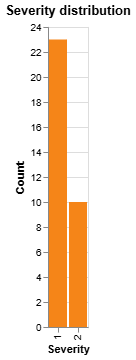
\includegraphics[width=\linewidth]{figures/severity_distribution.png}
\caption*{(a) Severity}
\end{minipage}
\hfill
\begin{minipage}{0.15\linewidth}
\centering
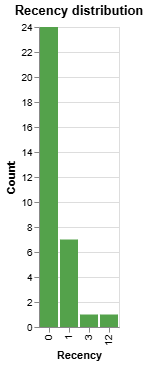
\includegraphics[width=\linewidth]{figures/recency_distribution.png}
\caption*{(b) Recency}
\end{minipage}
\hfill
\begin{minipage}{0.65\linewidth}
\centering
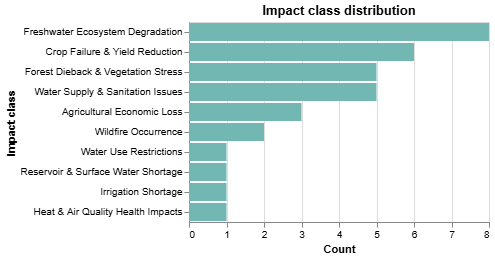
\includegraphics[width=\linewidth]{figures/impact_class_distribution.png}
\caption*{(c) Impact categories}
\end{minipage}

\caption{Distribution of event-level attributes and impact categories in the evaluation dataset.}
\label{fig:label_severity_recency_distributions}
\end{figure}

The impact category distribution is uneven, with agriculture, water resources, ecosystems, and forest-related impacts occurring most frequently. This reflects both newspaper reporting patterns and the event definition used in this study. Articles often describe the same type of impact across multiple locations, resulting in multiple annotated events within a single impact category. For example, a single article describing freshwater ecosystem degradation across several municipalities will produce multiple events, as each affected location is annotated separately. One single article has the potential to skew this entire distribution. Although the dataset does not provide equal representation across all impact categories, it contains sufficient diversity to compare LLM extraction performance.

% ------------------------------------------------

% \section{Comparison Setup and Model Configurations [move to 5.1]}
% \label{sec:model_comparison}
% % \subsection{Evaluated Models}

% To evaluate the practical trade-off between extraction quality, structural consistency, and inference cost, a diverse set of Large Language Models (LLMs) was selected. The models were chosen to reflect different operational profiles relevant to structured drought impact extraction from news articles. These profiles include high-capability reasoning models, cost-efficient structured extraction models, and lightweight high-throughput systems. All models are accessed through cloud APIs and configured to return structured JSON outputs.

% \begin{table}[h!]
% \centering
% \caption{Overview and Costs of Evaluated Models (May 2026)}
% \label{tab:evaluated_models}
% \small
% \renewcommand{\arraystretch}{1.2}
% \begin{tabular}{llccp{5.2cm}}
% \hline
% \textbf{Provider} & \textbf{Model} & \textbf{Input / 1M} & \textbf{Output / 1M} & \textbf{Main Reason for Testing} \\ \hline
% Anthropic & Claude 4.6 Sonnet & \$3.00 & \$15.00 & Strong instruction following, long-context processing, and consistent performance on complex multi-step language tasks. \\
% OpenAI & GPT-5.4 mini & \$0.75 & \$4.50 & Fast, low-cost reasoning model with structured output support and large context capacity. \\
% Google & Gemini 3.1 Pro & \$2.00 & \$12.00 & High-capacity reasoning model used as a flagship benchmark for extraction quality. \\
% Google & Gemini 3.5 Flash & \$1.50 & \$9.00 & Faster inference model balancing extraction quality, latency, and cost. \\
% Google & Gemini 3.1 Flash-Lite & \$0.25 & \$1.50 & Low-cost model for evaluating minimum viable extraction performance. \\ \hline
% \end{tabular}
% \end{table}


% The selected models represent different trade-offs between reasoning capability, throughput, cost efficiency, and structured generation reliability. The cost of each model quantitively are summarised in Table ~\ref{tab:evaluated_models}, next to that we get the reason for it.

% Claude 4.6 Sonnet is evaluated as a high-capability language model specialised in robust textual interpretation. News articles describing drought impacts often contain indirect causal relations, overlapping temporal references, and geographically dispersed events. This model is tested for its ability to preserve semantic consistency while generating structured outputs under ambiguous conditions.

% GPT-5.4 mini is evaluated as a computationally efficient reasoning model with native support for structured outputs and tool-oriented workflows. The model supports large context windows while maintaining relatively low inference costs. This makes it particularly suitable for high-volume extraction scenarios in which structural consistency and scalability are important.

% Gemini 3.1 Pro serves as the highest-capability benchmark model within the evaluated Google model family. The model is included to evaluate whether increased reasoning capacity improves extraction quality for complex event descriptions involving multiple locations, severity indicators, and temporal references.

% Gemini 3.5 Flash is included as a lower-cost alternative designed for high-throughput inference. The model targets applications requiring reduced latency and operational cost while retaining performance levels close to larger flagship systems.

% Gemini 3.1 Flash-Lite is evaluated as an ultra low-cost extraction model intended for large-scale processing pipelines. The model is primarily used to analyse the minimum computational cost required to construct structured drought impact datasets while maintaining acceptable extraction quality.



% \subsection{Controlled Experimental Setup for Model Comparison}
% \label{sec:controlled_experimental_setup}

% To ensure fair comparison across models, the extraction pipeline is held constant across all experimental conditions. The objective is to isolate differences in output quality and cost efficiency to the underlying model behaviour rather than prompt design or preprocessing variation.

% All models are evaluated using the same system prompt and the same structured extraction schema defined in Section~\ref{Extraction Framework Design}. They are also all evaluated using the same evaluation set. No model-specific prompt adaptations or optimisations are applied. This ensures that each model operates under identical task specifications and output constraints.

% The input pipeline is also kept fixed across all experiments. Articles undergo the same preprocessing steps, and no additional filtering, reformatting, or content selection is applied at the model level. This guarantees that all models receive equivalent input representations.

% For the temperature across all models, we use 0, to reduce stochastic variation in outputs. In combination with the fixed schema enforcement layer, this ensures that observed differences reflect model capability rather than sampling variability or prompt sensitivity. The library little llmn is used facilitate this.


% Overall, this controlled setup enables a direct comparison of models under identical conditions, allowing systematic evaluation of extraction quality, structural validity, and inference cost across different model families.

% \subsection{Evaluation Dimensions}


% \subsubsection{Extraction Quality Metrics}

% Extraction quality is evaluated at the event level, where each predicted event is matched against a reference event. Let $\mathcal{E}^{(g)}$ denote the set of ground-truth events and $\mathcal{E}^{(p)}$ the set of predicted events for a given article.
% %Evaluation is performed after optimal one-to-one alignment between predicted and reference events, ensuring that each prediction is evaluated against at most one reference instance.

% \paragraph{Impact classification accuracy}
% Impact classification is evaluated as a categorical matching problem. For each aligned event pair $(e_i^{(p)}, e_i^{(g)})$, the model prediction is considered correct if the predicted class matches the ground-truth class exactly:

% \[
% \mathrm{Acc}_{class} = \frac{1}{N} \sum_{i=1}^{N} \mathbb{1}\big(c_i^{(p)} = c_i^{(g)}\big)
% \]

% where $c_i$ denotes the drought impact class and $N$ is the total number of aligned events.

% \paragraph{Severity agreement}
% Severity is treated as a low-cardinality ordinal variable $s \in \{1, 2, 3\}$. Given this restricted range, we evaluate performance using simple accuracy rather than error-based metrics such as MAE. This choice avoids over-penalising small ordinal deviations that are not meaningful at this scale:

% \[
% \mathrm{Acc}_{sev} = \frac{1}{N} \sum_{i=1}^{N} \mathbb{1}\big(s_i^{(p)} = s_i^{(g)}\big)
% \]

% \paragraph{Recency agreement}
% Recency is defined in discrete temporal bins expressed in months:
% \[
% r \in \{0, 1, 2, 3, 4, 5, 6, 12, 24\}
% \]

% To evaluate temporal correctness, we report both exact-bin accuracy and mean absolute error (MAE). The MAE captures how far predictions deviate in time:

% \[
% \mathrm{MAE}_{rec} = \frac{1}{N} \sum_{i=1}^{N} \left| r_i^{(p)} - r_i^{(g)} \right|
% \]

% In addition, exact agreement is defined as:

% \[
% \mathrm{Acc}_{rec} = \frac{1}{N} \sum_{i=1}^{N} \mathbb{1}\big(r_i^{(p)} = r_i^{(g)}\big)
% \]

% \paragraph{Location correctness}
% Location correctness evaluates whether the model extracts the correct location mention as it appears in the source text. Since the LLM is not responsible for geographic resolution or spatial standardisation, evaluation is restricted to textual agreement with the reference annotation.

% Let $l_i^{(p)}$ denote the predicted location string and $l_i^{(g)}$ the ground-truth location mention. Correctness is defined using a normalised exact match:

% \[
% \mathrm{Acc}_{loc} = \frac{1}{N} \sum_{i=1}^{N} \mathbb{1}\big(\mathrm{norm}(l_i^{(p)}) = \mathrm{norm}(l_i^{(g)})\big)
% \]

% where $\mathrm{norm}(\cdot)$ removes differences in casing, punctuation, and leading or trailing whitespace.

% Geographic resolution to NUTS-3 level is handled in a separate geocoding stage (in .. ) and is therefore excluded from this evaluation.

% \paragraph{Event detection success}
% Event detection evaluates whether the model correctly identifies the presence of at least one drought impact event in an article. Let $y^{(g)} \in \{0,1\}$ denote whether any event exists in the ground truth and $y^{(p)}$ the corresponding prediction. We define detection accuracy as:

% \[
% \mathrm{Acc}_{event} = \frac{1}{M} \sum_{j=1}^{M} \mathbb{1}\big(y_j^{(p)} = y_j^{(g)}\big)
% \]

% where $M$ is the number of evaluated articles.

% Together, these metrics capture both semantic correctness (impact class, severity, recency, location) and the model’s ability to detect whether relevant events exist at all. This separation allows us to distinguish between extraction quality and extraction completeness, which is critical for evaluating large language models in structured information extraction tasks.

% % Main evaluation axis.
% %
% % Suggested metrics:
% % - impact classification accuracy
% % - severity agreement
% % - recency agreement
% % - location mention correctness
% % - event detection success
% %
% % Keep metrics simple.
% % Avoid overengineering unless dataset size supports it.
% %
% % Mention:
% % evaluation occurs at event level.

% \subsubsection{Structural Validity Metrics}

% to do needs work, didn't think this out yet enough.

% All models generate outputs under the same structured schema. Because of this, we mainly check whether the output can be correctly parsed into the required format.

% Let $N$ be the total number of model outputs. We define a binary variable $v_i$, where $v_i = 1$ if the output can be parsed successfully into the target schema, and $v_i = 0$ otherwise. Structural validity is then:

% \[
% \mathrm{Validity} = \frac{1}{N} \sum_{i=1}^{N} v_i
% \]

% An output is counted as valid if it follows the required structure and contains all required fields. If parsing fails or fields are missing, it is counted as invalid.

% Because all models are forced to follow the same schema, we expect this score to be very high in most cases. This metric mainly ensures that the pipeline works correctly and that no structural errors occur during generation.

% \subsubsection{Inference Cost and Computational Efficiency}
% %Later after running the code and having the dataset


% % Keep lightweight.
% %
% % Suggested measures:
% % - average inference time per article
% % - approximate API cost per article / dataset
% %
% % Do NOT overfocus on benchmarking hardware.
% %
% % Goal:
% % practical feasibility for large-scale extraction.

% \subsection{Aggregation and Comparative Evaluation}

% To compare models fairly, all evaluation metrics are computed at the event level and then aggregated across the full dataset. Each predicted event is matched with a reference event, and scores are calculated per event before averaging.

% Let $M$ be the number of matched events, and let $s_i$ denote the score for event $i$. The overall performance for a given metric is computed as:

% \[
% \mathrm{Score} = \frac{1}{M} \sum_{i=1}^{M} s_i
% \]

% % Final results are reported using simple averages across all events. This includes the main extraction quality metrics (classification, severity, recency, and location correctness) as well as structural validity. This ensures that each model is evaluated under the same conditions and contributes equally to the final score. For recency, we use exact agreement accuracy, as this aligns more naturally with the averaging framework compared to mean absolute error (MAE). 
% \subsubsection{Evaluation Metrics [needs work later]}

% Model performance is evaluated using a series of precision-based metrics that measure extraction quality at increasing levels of detail.

% \paragraph{Relevance Precision}

% The first metric evaluates whether the model correctly identifies articles containing drought-related impacts. Articles are classified as \textit{relevant}, \textit{irrelevant}, or \textit{uncertain}. Relevance precision is defined as:

% \[
% P_{rel} = \frac{TP_{rel}}{TP_{rel} + FP_{rel}}
% \]

% where $TP_{rel}$ denotes the number of correctly identified relevant articles and $FP_{rel}$ denotes the number of articles incorrectly classified as relevant.

% \paragraph{Location-Impact Precision}

% Location-impact precision evaluates whether the model correctly extracts both the location and impact category. A prediction is considered correct only if both fields match the reference annotation.

% \[
% P_{LI} = \frac{TP_{LI}}{TP_{LI} + FP_{LI}}
% \]

% where $TP_{LI}$ is the number of correctly predicted location-impact tuples and $FP_{LI}$ is the number of incorrect or spurious tuples.

% \paragraph{Location-Impact-Severity Precision}

% This metric extends location-impact precision by additionally requiring the severity label to be correct.

% \[
% P_{LIS} = \frac{TP_{LIS}}{TP_{LIS} + FP_{LIS}}
% \]

% A tuple is counted as correct only if location, impact category, and severity all match the reference annotation.

% \paragraph{Location-Impact-Recency Precision}

% Finally, this metric evaluates whether the model correctly extracts location, impact category, and recency information simultaneously.

% \[
% P_{LIR} = \frac{TP_{LIR}}{TP_{LIR} + FP_{LIR}}
% \]

% A prediction is considered correct only if all three attributes match the reference tuple.

% \paragraph{Summary}

% Together, these metrics evaluate both the model's ability to identify relevant articles and its ability to extract increasingly detailed drought-impact information from text.





\section{LLM Extraction Performance}


The results are shown in Table~\ref{tab:model_performance}. Overall, the evaluated models achieve modest extraction performance. For the primary location-impact metric, F1-scores range from 0.190 to 0.462. Gemini 3.5 Flash achieves the highest precision (0.469), recall (0.455), and F1-score (0.462), clearly outperforming the other evaluated models.

Claude Sonnet 4.5 achieves the second-highest recall, with a recall of 0.273 for the primary metric. This suggests that the model identifies relatively many drought impact events but also produces many false positives, resulting in a lower precision and overall F1-score. Despite being the most expensive model evaluated, Claude Sonnet 4.5 does not achieve the best overall extraction performance.

When the stricter location-impact-severity-recency metric is used, performance decreases substantially for every model. Gemini 3.5 Flash again achieves the highest performance with an F1-score of 0.185, while the remaining models score between 0.024 and 0.119. This indicates that correctly identifying a drought impact event is considerably easier than correctly extracting all associated event attributes.

One possible explanation for the strong performance of Gemini 3.5 Flash is that it is particularly well suited to structured information extraction tasks. Unlike complex reasoning benchmarks, this task primarily requires accurate entity extraction, classification, and structured JSON generation. Gemini Flash is designed for high-throughput structured workloads, which may better match the requirements of the proposed extraction framework. Another possible source of bias is that Gemini 3.5 Flash was used as a supporting tool during the manual annotation process. Although all annotations were manually verified, this may have introduced a small preference towards the model's output style.

Finally, the relatively low scores across all models are likely influenced by ambiguity in the impact taxonomy. During annotation, each event was assigned a single impact category, while multiple categories may reasonably describe the same drought impact. For example, an event describing reduced water availability for agriculture could potentially be labelled as irrigation shortage, water use restrictions, or reservoir and surface water shortage, depending on interpretation. Because the evaluation requires an exact category match, these semantic overlaps reduce the reported performance even when the extracted information is largely correct. This ambiguity is investigated further in the following sections.

\begin{table}[h!]
\centering
\caption{Event-level extraction performance of the evaluated LLMs.}
\label{tab:model_performance}
\small
\begin{tabular}{lccc|ccc}
\hline
& \multicolumn{3}{c|}{\textbf{Location + Impact}} & \multicolumn{3}{c}{\textbf{Location + Impact + Severity + Recency}} \\
\textbf{Model} & \textbf{P} & \textbf{R} & \textbf{F1} & \textbf{P} & \textbf{R} & \textbf{F1} \\
\hline
Gemini 3.5 Flash      & \textbf{0.469} & \textbf{0.455} & \textbf{0.462} & \textbf{0.188} & \textbf{0.182} & \textbf{0.185} \\
Gemini 3.1 Pro        & 0.206 & 0.212 & 0.209 & 0.118 & 0.121 & 0.119 \\
Claude Sonnet 4.5     & 0.191 & \textbf{0.273} & 0.225 & 0.064 & \textbf{0.091} & 0.075 \\
Gemini 3.1 Flash-Lite & 0.242 & 0.242 & 0.242 & 0.061 & 0.061 & 0.061 \\
GPT-5.4 mini          & 0.157 & 0.242 & 0.190 & 0.020 & 0.030 & 0.024 \\
\hline
\end{tabular}
\end{table}





\label{sec:variable_performance}


%\subsection{Extraction Performance Overview}

\subsection{Category Ambiguity and Granularity}

The low performance across all models can partly be explained by the structure of the impact taxonomy itself. To interpret these findings, we consider the concept of fuzzy categories from fuzzy set theory, introduced by Zadeh. Fuzzy set theory describes categories without clear boundaries, meaning that an element can partially belong to multiple categories simultaneously. This concept is particularly relevant for natural language, where concepts are often not strictly separated.

Initially, drought impacts can be grouped into broad categories, such as agricultural, hydrological, and socio-economic impacts. However, these categories overlap in practice. For example, reduced water availability can directly cause agricultural losses, meaning that the same drought event can reasonably belong to both hydrological and agricultural categories. This overlap is illustrated in Figure~\ref{fig:fuzzy_5sets}.

A natural expectation is that increasing the number of categories would reduce ambiguity by creating more specific definitions. However, increasing category granularity does not remove ambiguity. Instead, broad overlaps between major categories are replaced by more specific overlaps between closely related categories, as illustrated in Figure~\ref{fig:fuzzy_20sets}.

\begin{figure}[h!]
\centering

\begin{subfigure}{0.49\linewidth}
\centering
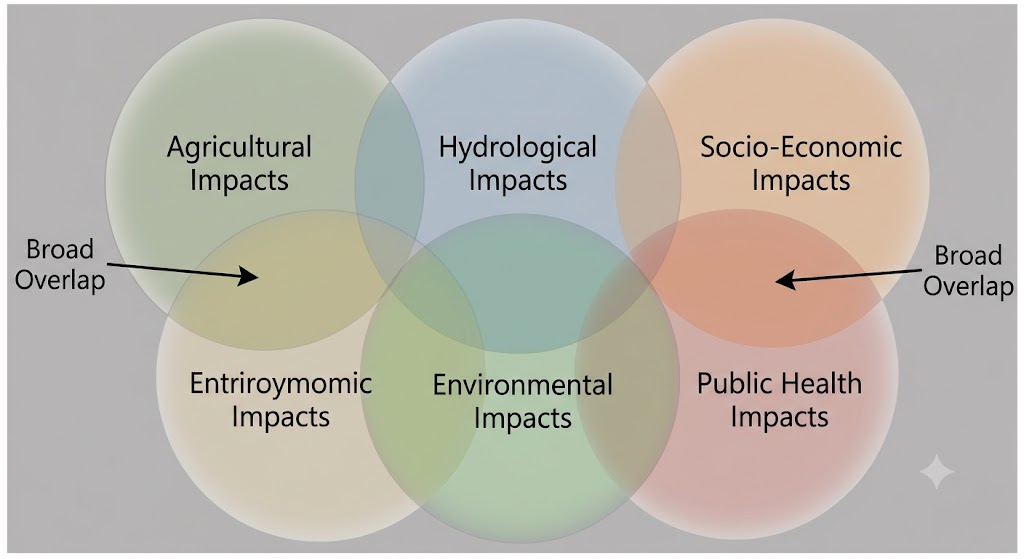
\includegraphics[width=\linewidth]{figures/Fuzzyset1.jpg}
\caption{Coarse-grained fuzzy impact categorisation (5 sets).}
\label{fig:fuzzy_5sets}
\end{subfigure}
\hfill
\begin{subfigure}{0.48\linewidth}
\centering
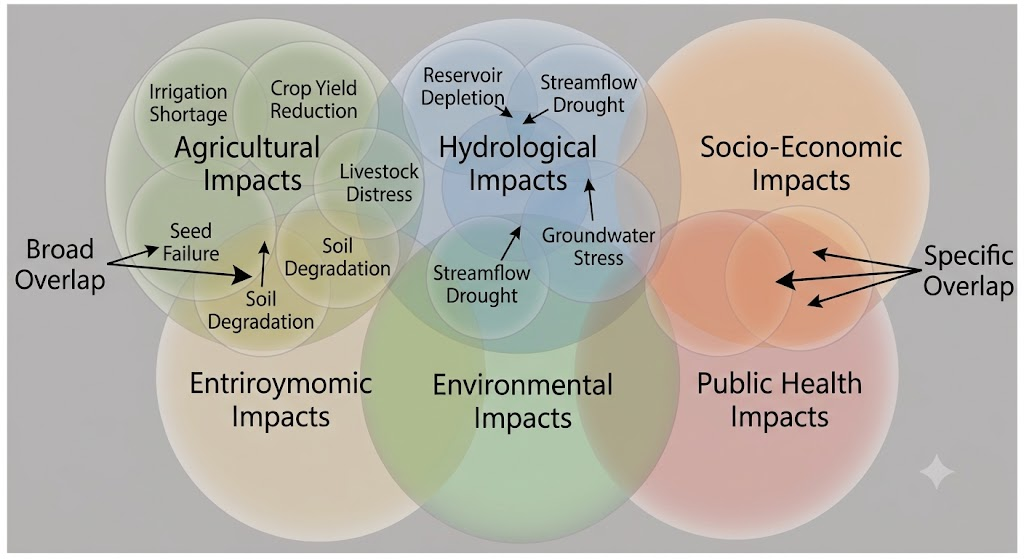
\includegraphics[width=\linewidth]{figures/Fuzzyset2.jpg}
\caption{Fine-grained fuzzy impact categorisation (20 sets).}
\label{fig:fuzzy_20sets}
\end{subfigure}

\caption{Comparison of coarse-grained and fine-grained fuzzy impact categorisations. Increasing category granularity changes the location of category overlap but does not remove ambiguity.}
\label{fig:fuzzy_comparison}
\end{figure}

For example, an article stating that farmers cannot irrigate because rivers have reached historically low water levels could reasonably be assigned to several categories, including irrigation shortage, reservoir and surface water shortage, water use restrictions, or agricultural impacts. However, annotation requires selecting a single ground-truth category. Therefore, a model prediction can be semantically correct while still being considered incorrect under strict evaluation.

This ambiguity is further increased by the event-level evaluation approach. A single drought impact may contain multiple related processes, but the evaluation requires an exact match between the predicted and annotated category. We attempted to account for this by allowing the model to extract multiple impacts for a single event, but in practice the model typically selected only the most dominant category.

\begin{figure}[h!]
\centering
\includegraphics[width=0.70\linewidth]{figures/Fuzzyset3.jpg}
\caption{Illustration of annotation ambiguity in the fine-grained impact categorisation.}
\label{fig:fuzzy_reality}
\end{figure}

Therefore, the relatively low extraction performance is not only caused by limitations of the language models but also by the difficulty of defining unique boundaries between drought impact categories. Figure~\ref{fig:fuzzy_reality} illustrates this challenge, where multiple categories can overlap for the same real-world drought impact. For example, the evaluation dataset contains many freshwater ecosystem degradation impacts, which could also reasonably be interpreted as surface water shortages in certain cases.

Future improvements could focus not only on improving model performance but also on developing annotation methods that allow multiple valid categories or different degrees of category membership.









\subsection{Post-hoc Evaluation and Structural Reformulation}

The previous evaluation showed that strict event-level matching can underestimate model performance when drought impacts have overlapping category boundaries. To further investigate this limitation, a post-hoc evaluation was performed on a subset of ten manually verified relevant articles. Instead of comparing predictions directly against a single ground-truth label, the extracted events were manually reviewed and classified as either correct, false positive, or false negative.

This evaluation provides a more direct assessment of whether the model identifies relevant drought impacts, independent of potential ambiguity in the predefined category labels. Therefore, it reduces the effect of strict category matching and allows us to distinguish between actual extraction errors and differences in interpretation between the model and the annotation.

In addition to the evaluation method, the extraction schema was reformulated to better represent the structure of drought impacts described in newspaper articles. The original formulation assumed that an article consists of multiple independent events, where each event represents a unique combination of location and impact category, together with additional attributes such as severity and recency. The model was therefore prompted to identify multiple events throughout the article.

However, this formulation does not fully reflect how drought impacts are commonly reported. A single location mention can describe several related impacts simultaneously. For example, an article discussing a drought-affected lake may mention reduced water levels, ecosystem degradation, and restrictions on water use at the same location.

The revised schema therefore follows a hierarchical structure. Instead of directly extracting independent events, the model first identifies location mentions and subsequently extracts all relevant impacts associated with each location. This formulation better represents the relationship between locations and impacts and reduces the need for the model to repeatedly search through the article for separate events.

The revised structure is:

\begin{itemize}
\item Article $\rightarrow$ Location mention
\item Location mention $\rightarrow$ Impact 1, Impact 2, Impact 3, ...
\item Each impact contains category, severity, recency, and supporting evidence
\end{itemize}

This reformulation is expected to improve the model's ability to identify multiple impacts associated with the same location and provides a more natural representation of drought impact reporting. The results of this post-hoc evaluation are presented in the following section.





\section{Post-hoc Results, and Model Selection}
\label{ch:Post-hoc Results}


\subsection{Impact categorization}
To further evaluate the quality of the extracted impacts, a post-hoc evaluation was performed on a subset of ten manually verified relevant articles. Instead of comparing model predictions against the predefined annotation labels, the extracted model outputs were manually reviewed and classified as either valid impact extractions or incorrect extractions. This evaluation focuses on whether the \textbf{impacts} identified by the models represent actual drought impacts described in the articles, while reducing the influence of strict category boundaries.

During the evaluation, one edge case was identified. One article described a potential public health hazard caused by drought conditions, where a lack of rainfall caused animal waste to accumulate before being transported into a lagoon by later rainfall. This article was classified as irrelevant because the drought created a vulnerability rather than a direct impact. Since the models were instructed to avoid making indirect assumptions, extracting this event was considered an incorrect extraction.

Additionally, extractions where the location was only specified as "the Netherlands" were excluded from the evaluation. This spatial resolution is too coarse for the regional impact analysis targeted in this study.

The results are shown in Table~\ref{tab:posthoc_results}. Claude Sonnet 4.5 and Gemini 3.5 Flash achieved the highest precision. Claude identified 26 valid impacts without producing any incorrect extractions, while Gemini 3.5 Flash identified the same number of valid impacts with two incorrect extractions. These results are consistent with the earlier event-level evaluation, where both models achieved the strongest overall performance.



\begin{table}[ht]
\centering
\caption{Post-hoc evaluation results based on manually verified model extractions.}\label{tab:posthoc_results}
\begin{tabular}{lrrr}
\toprule
Model & TP & FP & Precision \\
\midrule
Claude Sonnet 4.5      & 26 & 0  & 1.000 \\
Gemini 3.5 Flash       & 26 & 2  & 0.929 \\
Gemini 3.1 Flash Lite  & 16 & 4  & 0.800 \\
Gemini 3.1 Pro Preview & 18 & 5  & 0.783 \\
GPT-5.4 Mini           & 27 & 13 & 0.675 \\
\bottomrule
\end{tabular}
\end{table}















\subsection{Location, Severity, and Recency Extraction}

A secondary evaluation was performed on the two strongest-performing models to examine differences in individual extraction tasks, focusing on location extraction, severity classification, and recency estimation.

Differences were observed in the spatial resolution of extracted locations. Claude Sonnet 4.5 tended to assign more general spatial labels, such as "the Netherlands", whereas Gemini 3.5 Flash extracted more detailed regional information. For example, in an article discussing agricultural irrigation ("Sproeit die boer wel legaal"), Gemini extracted "Achterhoek", "Bolksbeek", and "Eibergen", while Claude only identified "Achterhoek".

A post-hoc spatial usability check was performed, where a location was considered a true positive if it could be mapped to a geographical region suitable for regional analysis. This criterion was not explicitly included in the extraction prompt. Both models produced five locations that could not be mapped to standard NUTS regions, such as "zandgebieden in Nederland" in the Gemini output. After filtering these cases, Gemini produced 17 usable locations compared to 14 from Claude, indicating more detailed spatial extraction within this evaluation sample.

Differences were also observed in severity and recency classification. Claude Sonnet 4.5 showed a tendency to assign higher severity scores than suggested by the annotation criteria, with several minor impacts classified as severity level 3. Additionally, Claude incorrectly assigned an "ongoing" recency label to an event that occurred in September but was reported at the end of October.

The attribute-level extraction performance is shown in Table~\ref{tab:extraction_performance}. A true positive represents a correct extraction according to the manual evaluation criteria, while a false negative represents a missed or incorrectly assigned attribute.

\begin{table}[htbp] 
\centering 
\caption{Attribute-level extraction performance of the evaluated models.} 
\label{tab:extraction_performance} 
\begin{tabular}{lrrrrrr} 
\toprule 
Model & Loc. TP & Loc. FN & Sev. TP & Sev. FN & Rec. TP & Rec. FN \\
\midrule 
Gemini 3.5 Flash & 17 & 5 & 24 & 0 & 14 & 0 \\
Claude Sonnet 4.5 & 14 & 5 & 29 & 5 & 14 & 1 \\
\bottomrule 
\end{tabular} 
\end{table}

Based on the combined event-level, post-hoc, and attribute-level evaluations, Gemini 3.5 Flash was selected as the final model. It provided more detailed spatial outputs and comparable extraction performance while having substantially lower inference costs.



% ==========================================
\chapter{Geocoding}

In this chapter, we geocode the location mentions extracted by the LLMs. The research questions addressed is:
How can a hierarchical geocoding pipeline be constructed to translate informal textual location references into NUTS-3 representations?
\label{ch:geocoding}
% ==========================================

\section{Geocoding Pipeline}

The LLM extraction framework produces location mentions as free-text descriptions. However, these textual locations cannot directly be used for spatial analysis because newspaper articles often contain ambiguous descriptions rather than standard administrative names. Therefore, a hierarchical geocoding pipeline was developed to translate textual location mentions into spatial representations.

The pipeline produces two outputs. First, each location mention is assigned a point location represented by latitude and longitude in the global WGS84 coordinate system. Second, each mention is assigned to one or more NUTS-3 regions. NUTS (Nomenclature of Territorial Units for Statistics) is the European standard for administrative regions. In this study, NUTS-3 regions are used because they provide sufficient spatial resolution for regional analysis and later machine learning applications.

The pipeline operates on unique location mentions extracted by the LLM. When the same location appears in multiple articles, it is geocoded once and reused. This reduces redundant searches and improves computational efficiency.

\subsection{Challenges in Location Geocoding}

Geocoding newspaper-derived location mentions introduces several challenges that are not present when working with structured geographic data. A first challenge is ambiguity in geographic names. A location mention can refer to different types of places, such as municipalities, neighbourhoods, streets, or small geographic features. For example, initial testing showed that the location mention ``Jordaan'' could be incorrectly matched to Jordaan Street, while the article referred to the Jordaan River.

A second challenge is the variation in spatial scale used by newspapers. Some articles refer to specific municipalities, whereas others describe provinces or broader regions. For example, a drought impact reported in ``Noord-Brabant'' does not necessarily refer to one specific municipality but rather to a wider area containing multiple NUTS-3 regions.

Finally, journalistic descriptions do not always correspond to official administrative units. Mentions such as ``zandgebieden in Nederland'' or ``het oosten van Nederland'' describe meaningful geographic areas but cannot directly be linked to a single administrative region.

To address these challenges, the pipeline follows a hierarchical approach in which increasingly general methods are applied only when more specific assignments cannot be made.


\subsection{Point-Level Geocoding}

The first step converts textual location mentions into geographic coordinates. Point-level geocoding answers the question: ``Where should this location mention be placed on the map?'' It does not directly determine the corresponding administrative regions.

Location mentions are matched using the OpenStreetMap Nominatim gazetteer service. The gazetteer returns possible geographic candidates together with coordinates and additional metadata. Initial testing showed that unrestricted matching could produce incorrect results, particularly for ambiguous names. Therefore, an additional ranking step was introduced to prioritise meaningful geographic matches.

The ranking procedure reorders candidate locations based on their geographic relevance. Administratively meaningful locations, such as municipalities, provinces, and recognised regions, are prioritised over less useful matches such as streets, buildings, or small geographic features. If an initial search returns an unsuitable match, a second search restricted to the Netherlands is performed.

The final point-level output contains the latitude and longitude of the selected location. These coordinates are later combined with drought impact information and are mainly used for map inspection and validation.

% \subsection{NUTS-3 Regional Assignment}

% While point geocoding answers where a mention is located, regional assignment determines which official regions should be associated with a drought impact. This step is required because regional datasets and predictive models require consistent administrative units rather than individual coordinates.

% The NUTS-3 assignment uses the geocoded point location together with additional text-based rules. Official EU NUTS 2021 boundaries for the Netherlands are used to assign locations to administrative regions.

% The assignment process follows a hierarchical decision structure (Figure~\ref{fig:nuts3-flow}). After filtering invalid, non-Dutch, and country-level mentions, the pipeline first attempts text-based matching. Within this step, direct NUTS-3 name matches are prioritised. If no direct match is found, broader regional descriptions are considered, including NUTS-2 aliases and macro-regional phrases. These broader mentions are subsequently decomposed into their corresponding NUTS-3 regions. If no text-based match is possible, the pipeline falls back to coordinate-based assignment, where the geocoded point is checked against NUTS-3 polygons. If the point falls within a polygon, the corresponding region is assigned. This hierarchical order prioritises explicit textual information over spatial approximation.

\subsection{NUTS-3 Regional Assignment}

While point geocoding answers where a mention is located, regional assignment determines which official regions should be associated with a drought impact. This step is required because regional datasets and predictive models require consistent administrative units rather than individual coordinates.

The NUTS-3 assignment uses the geocoded point location together with additional text-based rules. Official EU NUTS 2021 boundaries for the Netherlands are used to assign locations to administrative regions.

The assignment process follows a hierarchical decision structure (Figure~\ref{fig:nuts3-flow}). After filtering invalid, non-Dutch, and country-level mentions, the pipeline first attempts text-based matching. Within this step, direct NUTS-3 name matches are prioritised. If no direct match is found, broader regional descriptions are considered, including NUTS-2 aliases and macro-regional phrases. These broader mentions are subsequently decomposed into their corresponding NUTS-3 regions. If no text-based match is possible, the pipeline falls back to coordinate-based assignment, where the geocoded point is checked against NUTS-3 polygons. If the point falls within a polygon, the corresponding region is assigned. If the geocoded point does not fall inside a NUTS-3 polygon, the nearest NUTS-3 region within 25 km is assigned.
This hierarchical order prioritises explicit textual information over spatial approximation.

\begin{figure}[htbp]
\centering
% Added scale=0.75 and transform shape to "zoom out"
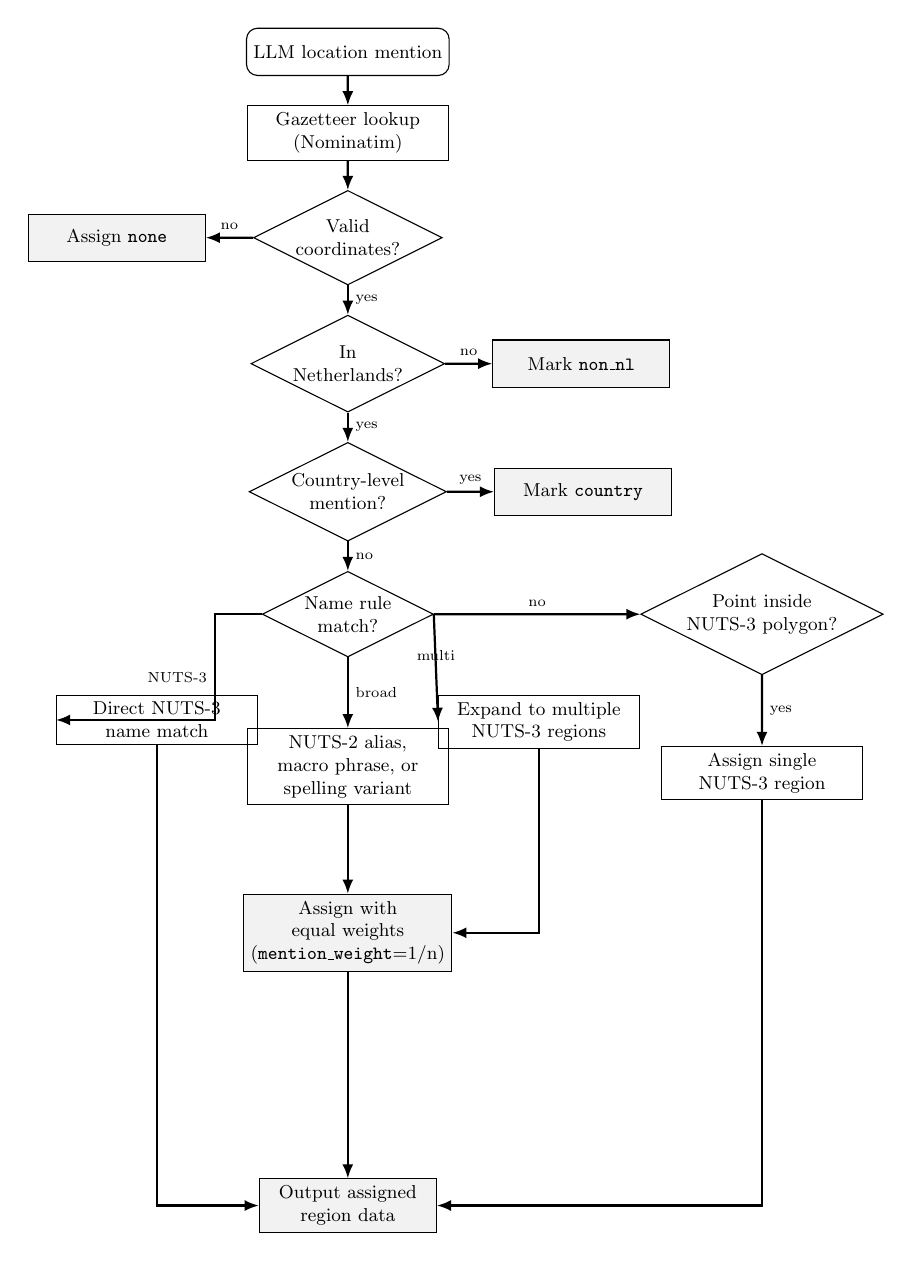
\begin{tikzpicture}[
  scale=0.75, transform shape, 
  node distance=5mm and 6mm, % Tightened spacing
  startstop/.style={rectangle, rounded corners, draw, align=center, minimum width=30mm, minimum height=8mm, font=\small},
  process/.style={rectangle, draw, align=center, minimum width=34mm, minimum height=8mm, font=\small},
  decision/.style={diamond, aspect=2, draw, align=center, inner sep=1pt, font=\small},
  result/.style={rectangle, draw, align=center, minimum width=30mm, minimum height=8mm, font=\small, fill=gray!10},
  arrow/.style={-{Latex[length=1.8mm,width=1.4mm]}, thick}
]

% Main Vertical Spine
\node[startstop] (input) {LLM location mention};
\node[process, below=of input] (geo) {Gazetteer lookup\\(Nominatim)};
\node[decision, below=of geo] (d1) {Valid\\coordinates?};
\node[decision, below=of d1] (d2) {In\\Netherlands?};
\node[decision, below=of d2] (d3) {Country-level\\mention?};
\node[decision, below=of d3] (d4) {Name rule\\match?};

% Exclusion Side Terminals - Reduced offset to 8mm
\node[result, left=8mm of d1] (none) {Assign \texttt{none}};
\node[result, right=8mm of d2] (nonnl) {Mark \texttt{non\_nl}};
\node[result, right=8mm of d3] (country) {Mark \texttt{country}};

% Name Rule Sub-Branches (Horizontal Row below d4)
\node[process, below left=10mm and 8mm of d4] (name1) {Direct NUTS-3\\name match};
\node[process, below=12mm of d4] (name2) {NUTS-2 alias,\\macro phrase, or\\spelling variant};
\node[process, below right=10mm and 8mm of d4] (name3) {Expand to multiple\\NUTS-3 regions};

% Geometry Fallback Branch - Reduced right offset to 35mm
\node[decision, right=35mm of d4] (d5) {Point inside\\NUTS-3 polygon?};
\node[process, below=12mm of d5] (single) {Assign single\\NUTS-3 region};

% Consolidated Actions & Terminal Endpoints
\node[result, below=15mm of name2] (weighted) {Assign with\\equal weights\\(\texttt{mention\_weight}=1/n)};
\node[result, below=35mm of weighted] (out) {Output assigned\\region data};

% Arrows - Main Spine & Exclusions
\draw[arrow] (input) -- (geo);
\draw[arrow] (geo) -- (d1);
\draw[arrow] (d1) -- node[above, font=\scriptsize]{no} (none);
\draw[arrow] (d1) -- node[right, font=\scriptsize]{yes} (d2);
\draw[arrow] (d2) -- node[above, font=\scriptsize]{no} (nonnl);
\draw[arrow] (d2) -- node[right, font=\scriptsize]{yes} (d3);
\draw[arrow] (d3) -- node[above, font=\scriptsize]{yes} (country);
\draw[arrow] (d3) -- node[right, font=\scriptsize]{no} (d4);

% Arrows - Name Rule Splits
\draw[arrow] (d4.west) -- ++(-0.8,0) |- node[pos=0.3, left, font=\scriptsize]{NUTS-3} (name1.west);
\draw[arrow] (d4) -- node[right, font=\scriptsize]{broad} (name2);
\draw[arrow] (d4.east) -- node[above, font=\scriptsize]{multi} (name3.west);

% Arrows - Name Rules to Endpoints
\draw[arrow] (name1.south) |- (out.west);
\draw[arrow] (name2) -- (weighted);
\draw[arrow] (name3.south) |- (weighted.east);

% Arrows - Geometry Fallback Branch
\draw[arrow] (d4) -- node[above, font=\scriptsize]{no} (d5);
\draw[arrow] (d5) -- node[right, font=\scriptsize]{yes} (single);
% \draw[arrow] (d5.east) -- node[above, font=\scriptsize]{no} ++(0.8,0) |- (weighted.east);

% Final resolution flows to Output
\draw[arrow] (single.south) |- (out.east);
\draw[arrow] (weighted) -- (out);

\end{tikzpicture}
\caption{NUTS-3 assignment logic. The flowchart shows the decision path from gazetteer lookup through text-based rules and polygon checks.}
\label{fig:nuts3-flow}
\end{figure}

\newpage
\subsection{Difference Between Point and Regional Outputs}

Although both outputs originate from the same geocoding process, they serve different purposes. Point locations preserve the original spatial position of the extracted mention and are mainly used for visual inspection and validation. NUTS-3 assignments convert textual locations into consistent regional units that can be aggregated and combined with external datasets.

The regional representation is therefore used for predictive modelling. By assigning impacts to NUTS-3 regions, regional drought characteristics and external variables can be linked consistently across different locations.

\label{ch:geocoding_pipe}

\newpage
\chapter{Visualization and Dataset Reliability}
In this chapter, we visualise the extracted drought impact data and conduct a reliability analysis. The research question addressed in this chapter is:

Which systematic biases, including regional reporting differences and environmental factors, affect the correspondence between news-derived impact data and reference datasets?

\section{Visualization of Extracted Impact Data}
After geocoding, drought impacts are stored as tables with coordinates or region codes. These tables are hard to interpret on their own. An interactive map viewer was built to display the geocoded dataset in spatial form and support manual inspection before the validation analysis in the next section.

\subsection{Purpose}

The viewer was designed with three main aims.

The first aim is to check whether extracted impacts are credible. A user can inspect where impacts appear on the map, whether locations look reasonable for the Netherlands, and whether the extracted impact fields match the source news text. This combines spatial checking and text checking in one workflow.

The second aim is to study patterns across impact classes. The map can be restricted to one or more drought-impact categories (for example crop failure, groundwater depletion, or wildfire stress). Because each class keeps a fixed map colour, class-specific spatial patterns become easier to compare.

The third aim is to study patterns over time. Impacts are linked to article publication month, and the map can be limited to a selected period. This supports inspection of when certain impacts were reported, rather than only where they occurred.

\subsection{Point-Level Map}

\begin{figure}[htbp]
\centering
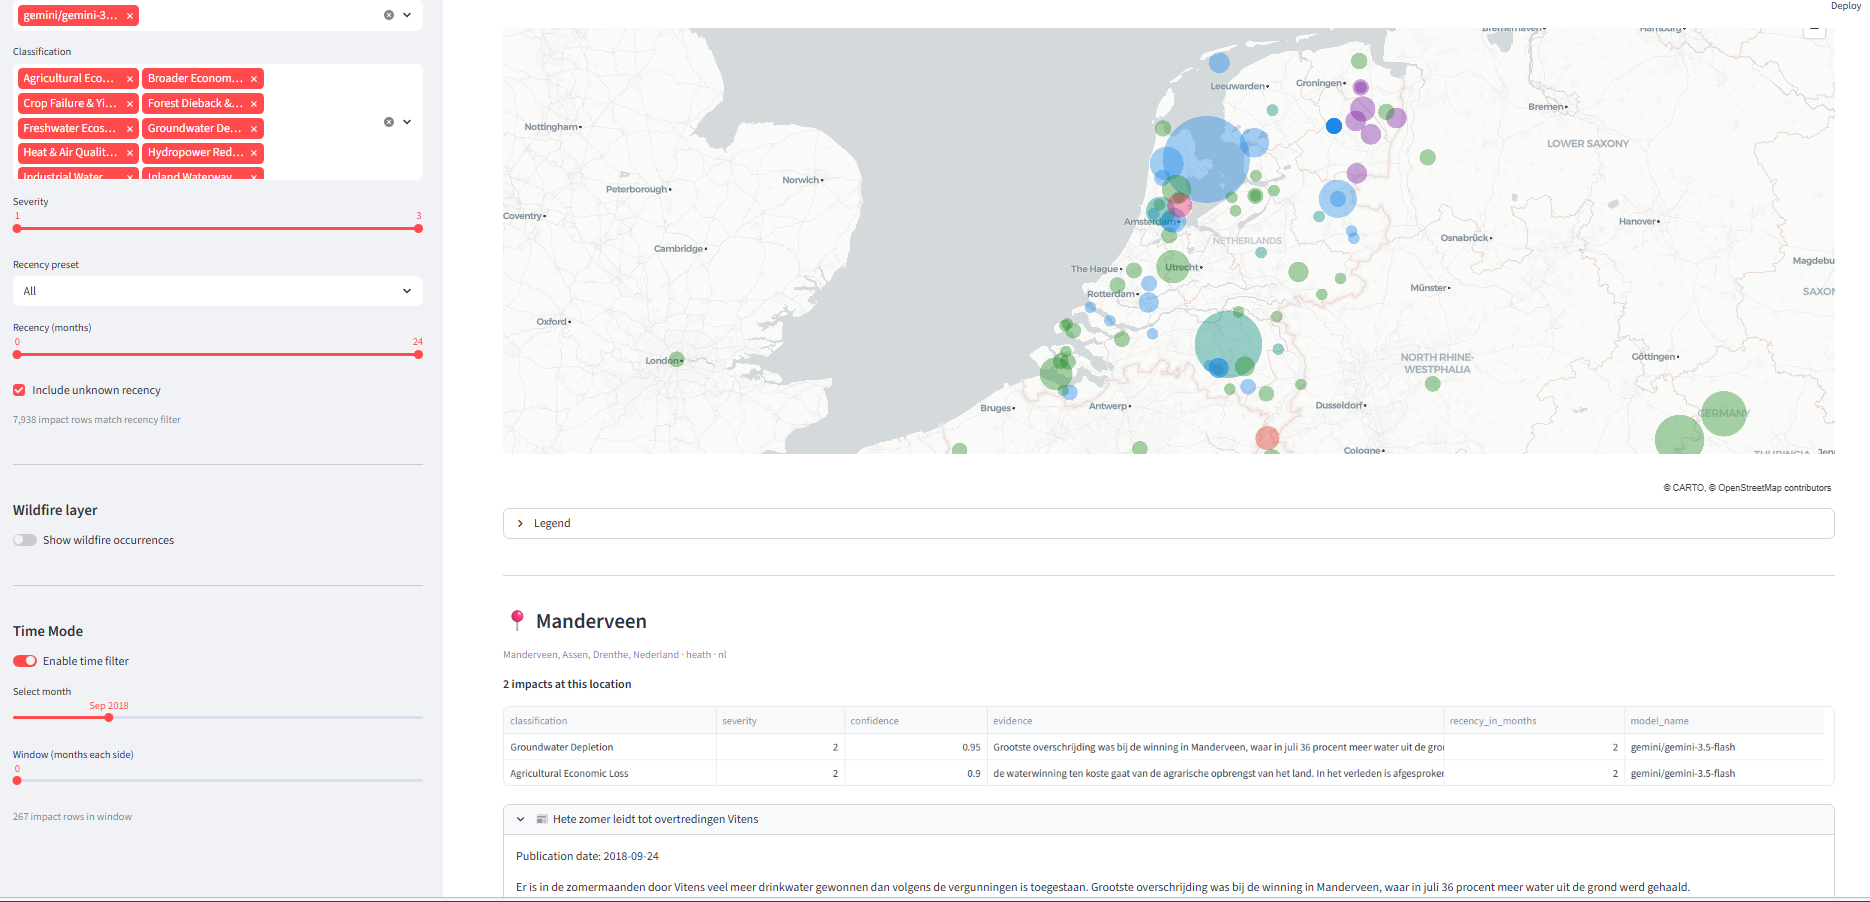
\includegraphics[width=0.97\textwidth]{figures/tool-overvieuw 2.png}
\caption{Point map and the news article view below.}
\label{fig:point-map}
\end{figure}

The point map displays geocoded impacts as markers on a Netherlands basemap (Figure~\ref{fig:point-map}). Impacts that share the same location mention are grouped into one marker. The number of impacts at a location controls marker size: places with more reported impacts appear as larger dots. Marker colour shows the dominant impact theme at that location. The original 20 impact classes are aggregated into six thematic groups: Agriculture (green), Water (blue), Fire and Heat (red-orange), Ecosystem (teal), Economy (purple), and Social (rose) (Table~\ref{tab:theme-colours}).

Marker transparency reflects the dominance of the leading impact theme. Locations where most impacts belong to a single theme appear more opaque, while locations with a more mixed impact profile appear fainter.

\begin{table}[htbp]
\centering
\caption{Thematic colour scheme used in the map viewer. The original 20 LLM impact labels are aggregated into six theme families.}
\label{tab:theme-colours}
\begin{tabular}{lll}
\toprule
Theme Family & Colour & Example Classes \\
\midrule
Agriculture & Green & Crop Failure, Irrigation Shortage, Agricultural Economic Loss \\
Water & Blue & Groundwater, Reservoir, Water Supply, Hydropower \\
Fire \& Heat & Red-orange & Wildfire Occurrence, Wildfire Risk, Heat \& Air Quality \\
Ecosystem & Teal & Freshwater Ecosystem, Forest Dieback, Wetland Loss \\
Economy & Purple & Broader Economic Disruption \\
Social & Rose & Social Impacts \\
\bottomrule
\end{tabular}
\end{table}



This view is suited to local inspection. It shows whether many impacts collapse onto the same place name, whether coordinates fall inside or outside the Netherlands, and whether geocoding appears too broad or too specific. Selecting a location opens a detail view with the impact records at that place and, when available, the related article text.

\subsection{Regional NUTS-3 Map}

\begin{figure}[htbp]
\centering
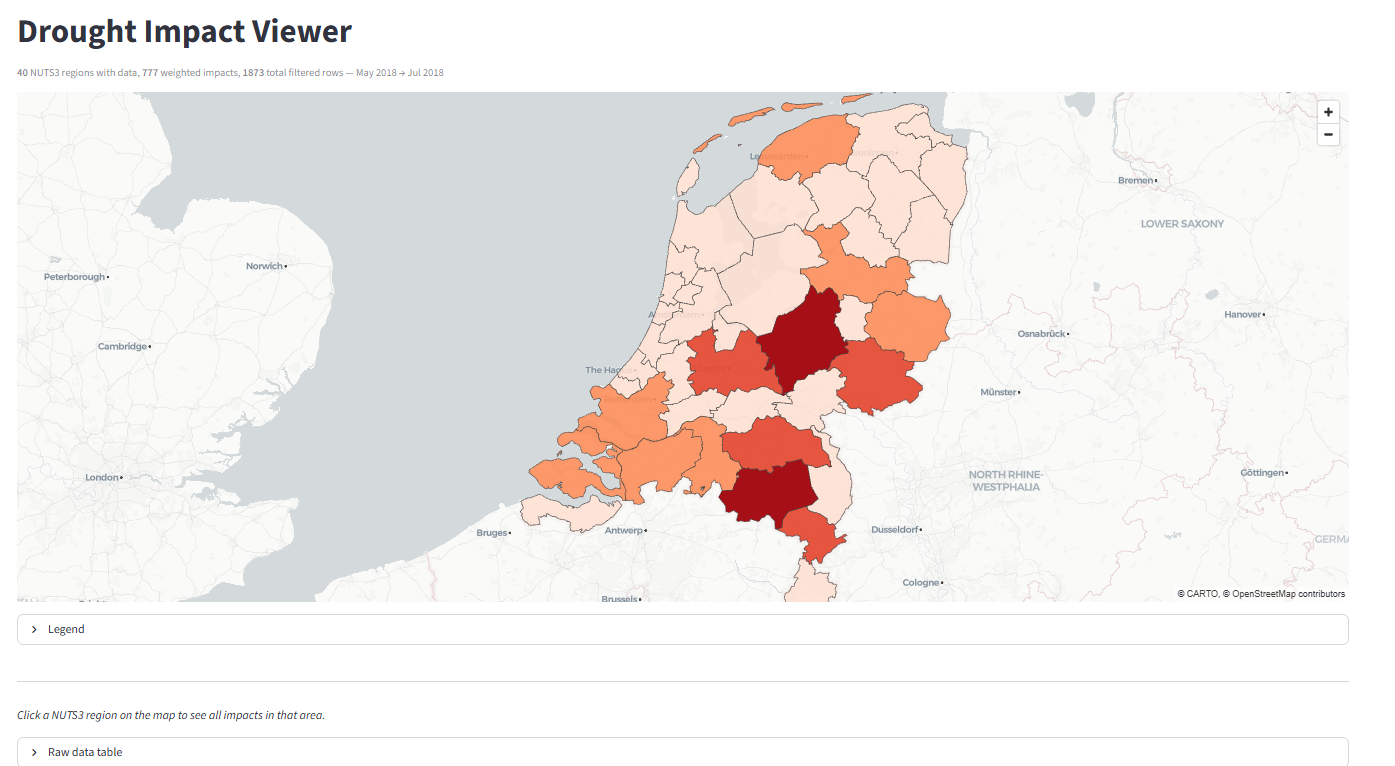
\includegraphics[width=0.8\textwidth]{figures/nuts-vieuw.png}
\caption{The NUTS-3 viewer with choropleth path colours}
\label{fig:nuts3-map}
\end{figure}

The regional map displays impacts on official NUTS-3 boundaries (Figure~\ref{fig:nuts3-map}). Impacts assigned to the same region are combined into one regional total. When a mention was split across multiple regions during geocoding, each part is counted through its \texttt{mention\_weight}, so broad phrases do not count as full impacts in every region.

Regional shading uses a colour scale from light to dark red. Regions with few or no impacts stay pale. Regions with more weighted impacts become darker. This makes regional concentration visible at a glance. Selecting a region shows the impacts assigned to that NUTS-3 unit and the linked article text where available.

The point map emphasises individual locations and local clustering. The regional map emphasises province-level structure and is better aligned with regional data used later in the thesis.

\subsection{Temporal and Class Views on the Map}

The same map can be filtered by impact class, severity, recency, and publication month. These filters change which markers or regions are drawn, not only which rows appear in a table. In practice, this allows class-specific maps for one drought category and month-specific maps for a chosen reporting window.

An optional wildfire layer can be added on top of either map. It shows observed fire occurrences from an external dataset and is included only as background context when inspecting drought-related fire reporting.

The next section uses these map views to assess geocoding quality and describe spatial and temporal patterns in the extracted impact dataset.








\newpage
\section{External Validation Using a Wildfire Case Study}

In this subsection, a wildfire dataset is used to compare the drought impact database with reported wildfire occurrences.

\subsection{Exploratory Data Analysis}

\begin{figure}[htbp]
\centering
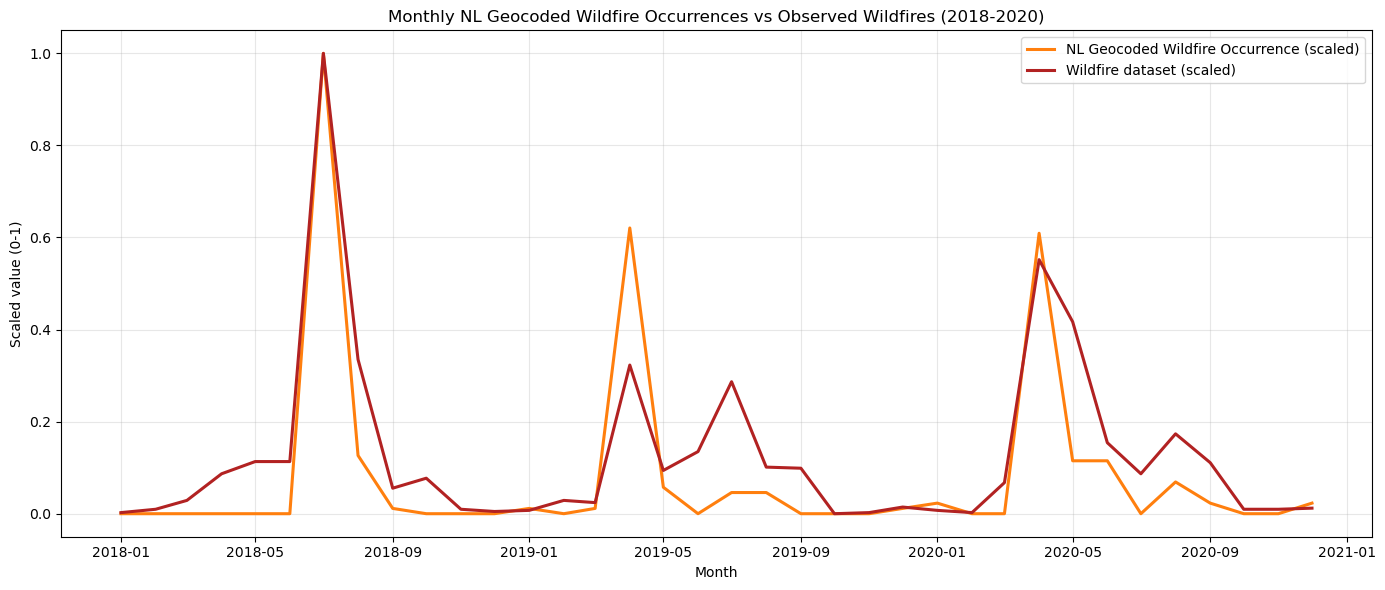
\includegraphics[width=0.95\textwidth]{figures/Monthly NL Geocoded Wildfire Occurrences vs Observed Wildfires (2018-2020).png}
\caption{Monthly normalized NL-geocoded wildfire occurrences compared with observed reference wildfires from 2018 to 2020.}
\label{fig:fires}
\end{figure}

As an initial evaluation, the wildfire events extracted by the LLM were compared with a separate wildfire reference dataset for the Netherlands. The reference dataset contains fire department call records and therefore represents reported wildfire occurrences rather than the size or severity of the fires. Monthly wildfire counts from both datasets were compared between January 2018 and December 2020.

Because both datasets use different scales, the two time series were separately transformed using min--max normalization to values between $[0,1]$. This allows comparison of changes over time rather than differences in the absolute number of events.

As shown in Figure~\ref{fig:fires}, both datasets show similar seasonal patterns, with a clear peak during the summer of 2018. The LLM-extracted wildfire series captures most peaks observed in the reference dataset during the following summers. However, a clear difference occurs in July 2019, where the reference dataset shows a strong increase in wildfire occurrences that is not visible in the extracted dataset. This period is therefore investigated further in the case study analysis. Overall, both datasets show similar temporal patterns after normalization.


\subsection{Case Study Analysis}

Based on the exploratory analysis, three periods were selected for further investigation: the major wildfire peak of July 2018, the smaller wildfire peak of April 2019, and the missing wildfire peak of July 2019. These periods show examples where the extraction framework successfully captures wildfire activity and where differences between datasets occur.

The extracted wildfire events were compared with the reference wildfire dataset at a monthly level. For this analysis, the recency window was set to 0, meaning that only impacts classified as ongoing or occurring within the previous month were included. Only wildfire occurrence events were considered, while wildfire risk indicators were excluded to evaluate how well the framework captures actual wildfire events.

\paragraph{July 2018}

Figure~\ref{fig:wildfire-geocoding-comparison-jul2018} compares observed wildfire occurrences with wildfire events extracted from newspaper articles during July 2018. The point-level representation shows that extracted locations do not always exactly match the recorded wildfire locations. This is expected because newspapers often report municipalities, nature areas, or larger regions instead of exact coordinates.
\begin{figure}[!htbp]
\centering
\begin{subfigure}[t]{0.49\textwidth}
\centering
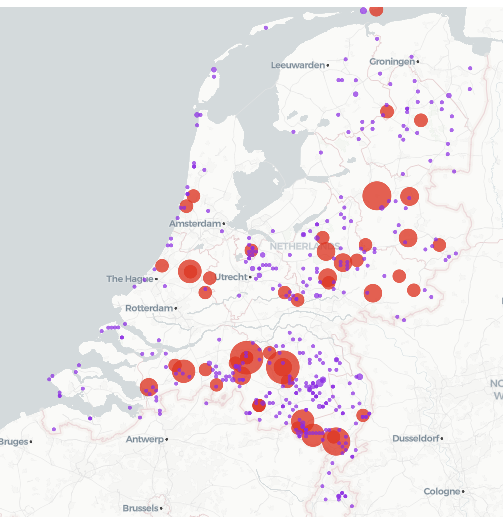
\includegraphics[width=\textwidth]{figures/Wildfires-Jul-2018-point.png}
\caption{Point-level geocoding results.}
\label{fig:wildfire-point-jul2018}
\end{subfigure}
\hfill
\begin{subfigure}[t]{0.49\textwidth}
\centering
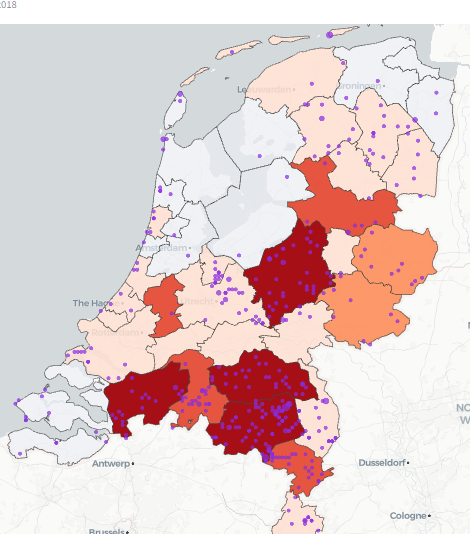
\includegraphics[width=\textwidth]{figures/Wildfires-Jul-2018-Nuts.png}
\caption{NUTS-3 aggregated geocoding results.}
\label{fig:wildfire-nuts-jul2018}
\end{subfigure}
\caption{Comparison of wildfire event locations extracted from news articles for July 2018 using point-level geocoding and NUTS-3 aggregation.}
\label{fig:wildfire-geocoding-comparison-jul2018}
\end{figure}

Despite these differences, most extracted locations are close to areas with recorded wildfire activity. This suggests that the extracted events generally correspond to real wildfire occurrences. After aggregation to the NUTS-3 level, regional wildfire patterns become easier to interpret. In particular, the higher wildfire concentrations in the southern Netherlands, especially North Brabant and surrounding regions, are captured reasonably well. 

The comparison also shows regions where fewer events are extracted compared with the reference dataset. For example, wildfire activity around Utrecht appears stronger in the reference dataset than in the newspaper-derived dataset. Possible explanations for these regional differences are discussed in Section~\ref{sec:spatial-differences}.

\paragraph{April 2019}

Figure~\ref{fig:wildfire-geocoding-comparison-apr2019} shows another period with good agreement between the extracted wildfire events and the reference dataset. Regions with more recorded wildfire occurrences generally also contain more extracted news events.

\begin{figure}[!htbp]
\centering
\begin{subfigure}[t]{0.49\textwidth}
\centering
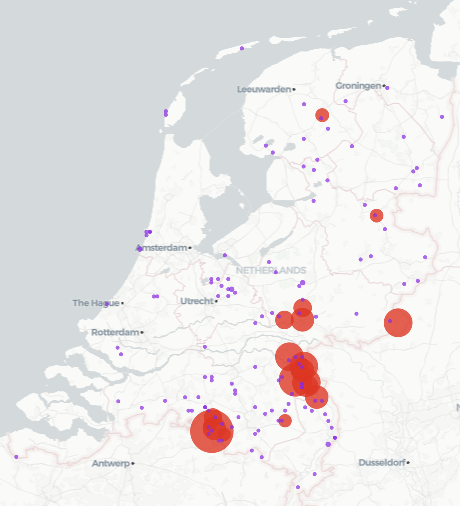
\includegraphics[width=\textwidth]{figures/Wildfires-April-2019-point.png}
\caption{Point-level geocoding results.}
\label{fig:wildfire-point-apr2019}
\end{subfigure}
\hfill
\begin{subfigure}[t]{0.49\textwidth}
\centering
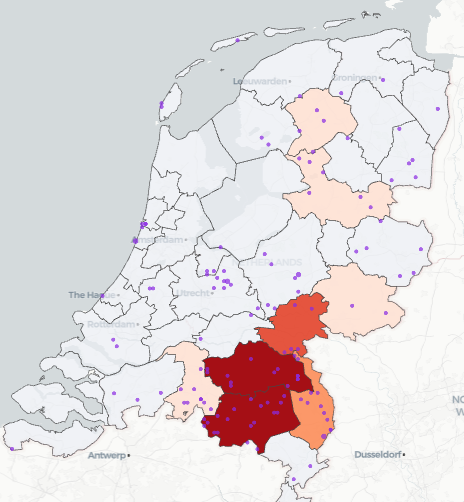
\includegraphics[width=\textwidth]{figures/Wildfires-April-2019-Nuts.png}
\caption{NUTS-3 aggregated geocoding results.}
\label{fig:wildfire-nuts-apr2019}
\end{subfigure}
\caption{Comparison of wildfire event locations extracted from news articles for April 2019 using point-level geocoding and NUTS-3 aggregation.}
\label{fig:wildfire-geocoding-comparison-apr2019}
\end{figure}

Similar to July 2018, Utrecht is underrepresented in the extracted dataset compared with the reference dataset. However, the overall spatial agreement remains strong, suggesting that newspaper-based wildfire extraction can capture regional wildfire patterns despite differences in reporting.

\paragraph{July 2019}

July 2019 shows the largest difference between the extracted wildfire events and the reference dataset. While the reference dataset contains many wildfire occurrences, only one newspaper-derived wildfire event was identified (Figure~\ref{fig:wildfire-geocoding-comparison-jul2019}).

\begin{figure}[!htbp]
\centering
\begin{subfigure}[t]{0.49\textwidth}
\centering
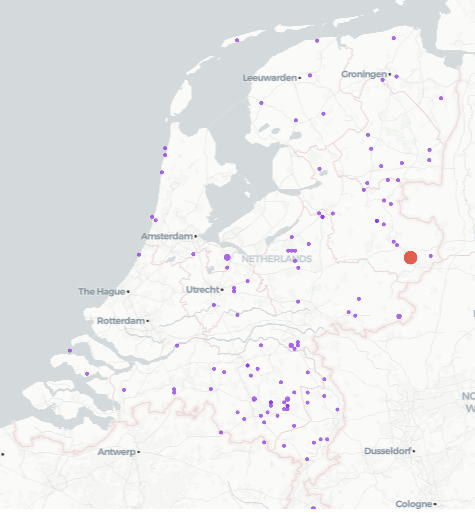
\includegraphics[width=\textwidth]{figures/Wildfires-July-2019-point.png}
\caption{Point-level geocoding results.}
\label{fig:wildfire-point-jul2019}
\end{subfigure}
\hfill
\begin{subfigure}[t]{0.49\textwidth}
\centering
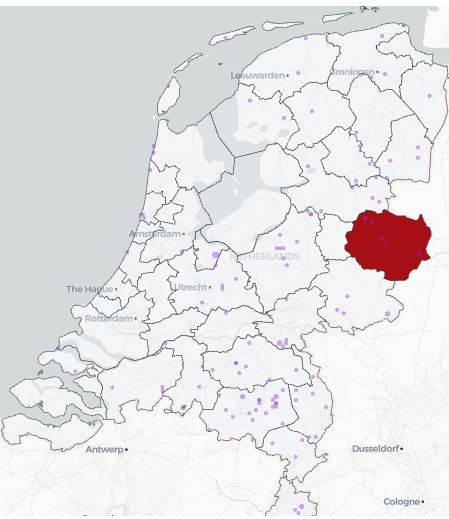
\includegraphics[width=\textwidth]{figures/Wildfires-July-2019-Nuts2.png}
\caption{NUTS-3 aggregated geocoding results.}
\label{fig:wildfire-nuts-jul2019}
\end{subfigure}
\caption{Comparison of wildfire event locations extracted from news articles for July 2019 using point-level geocoding and NUTS-3 aggregation.}
\label{fig:wildfire-geocoding-comparison-jul2019}
\end{figure}

Manual inspection showed that this article described a police investigation into suspected arson rather than a drought-related wildfire. Therefore, no direct drought-related wildfire impacts were extracted from the newspaper archive during this period. Since many drought-related articles were published during July 2019, this difference is unlikely to be caused by missing data collection.

One possible explanation is that newspapers do not report all wildfire occurrences. Fire department records may contain many small or local fires that are not considered important enough for news coverage. Therefore, the extracted dataset may represent reported wildfire impacts rather than all wildfire occurrences.

To investigate this limitation, the extraction was repeated while including both wildfire occurrence events and wildfire risk increase indicators. As shown in Figure~\ref{fig:graph-multiwildfire-risk-increase} and Figure~\ref{fig:wildfirerisk-increase-map}, the expanded dataset shows much closer agreement with the reference dataset.

\begin{figure}[!htbp]
    \centering
    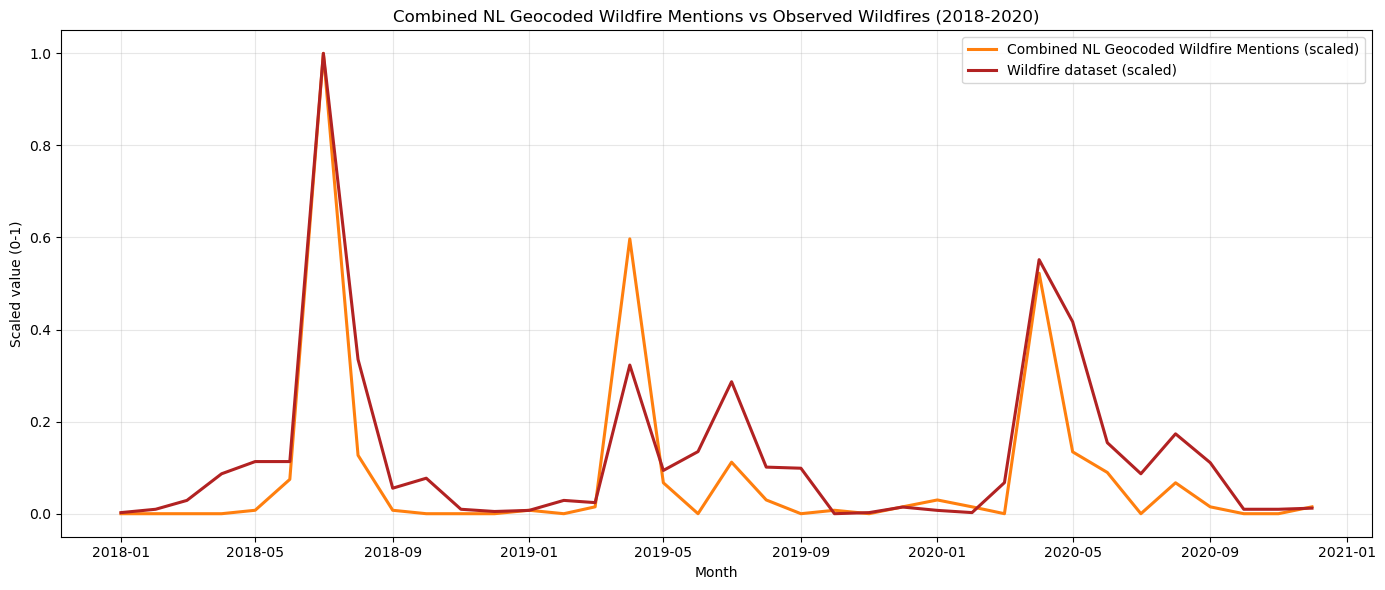
\includegraphics[width=0.75\linewidth]{figures/Wildfires-wildfire-risk increase.png}
    \caption{Normalized temporal comparison incorporating expanded wildfire risk indicators for July 2019.}
    \label{fig:graph-multiwildfire-risk-increase}
\end{figure}

\begin{figure}[!htbp]
    \centering
    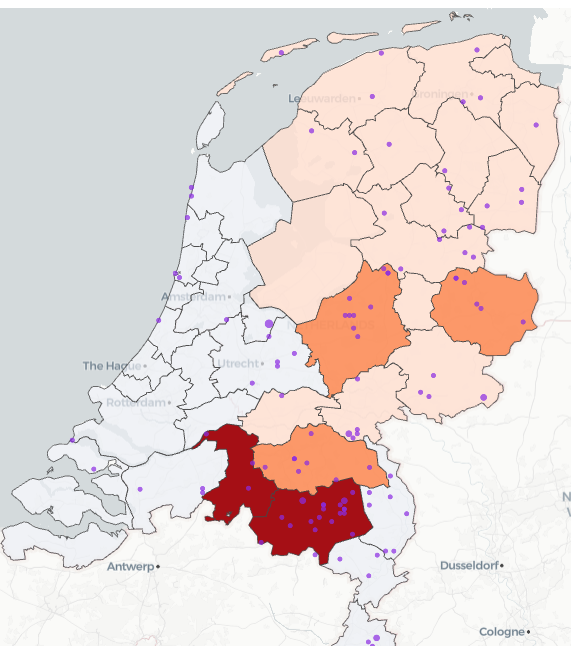
\includegraphics[width=0.30\linewidth]{figures/Wildfires-risk-increase-July-2019-nuts2.png}
    \caption{Spatial distribution of combined wildfire events and institutional risk warnings at the NUTS-3 level for July 2019.}
    \label{fig:wildfirerisk-increase-map}
\end{figure}

This indicates that newspaper-derived drought impact data can capture a broader wildfire-related signal, including periods of increased wildfire risk reported in newspapers, rather than only confirmed wildfire occurrences. This provides partial validation for the wildfire risk increase drought impact variable. It also demonstrates that there is a threshold before wildfire impacts are reported in newspapers compared with the reference dataset. Another hypothesis for this sudden mismatch in the data is that this was the second wildfire wave of the year and occurred during the summer holiday period. As a result, there may have been fewer journalists available to report on these events, leading to lower newspaper coverage despite wildfires occurring.



\subsection{Discussion of Spatial Reporting Differences}

In the previous section, we mentioned that fewer wildfires were observed in the Utrecht area during July 2018 in Fig. \ref{fig:wildfire-nuts-jul2018}.

After consulting with Femke Schasfoort, an expert on drought impacts in the Netherlands, we formulated several hypotheses to explain why substantially fewer wildfire impacts were identified in the Utrecht region during July 2018 and April 2019 compared to the reference dataset. An initial hypothesis was that the differences could be explained by soil type, as sandy soils are generally more vulnerable to wildfires. In Figure~\ref{fig:soil-type}, the Utrecht region appears to be predominantly covered by clay soils and therefore seems less vulnerable to wildfires. However, upon closer inspection, we found that the area within Utrecht where most wildfire impacts occurred in the reference dataset is actually located on sandy soils. This observation rejects the soil type hypothesis.

Another hypothesis relates to the reporting threshold discussed in the previous subsection. We concluded that wildfires likely need to exceed a certain threshold before they are reported in newspapers. It is possible that the wildfires occurring in the Utrecht region were relatively small or were effectively contained through government policies and efficient fire department responses. As a result, these events may never have reached the threshold required to be considered newsworthy, despite being included in the reference dataset. This explanation can be referred to as the reporting bias hypothesis or the rapid government response hypothesis. 

Overall, we observe clear correlations between the reference dataset, which records reported wildfire's, from any severity wildfires, and our impact dataset, which captures wildfires reported in newspaper articles. This indicates that both datasets have validity. However, the datasets do not match one-to-one due to reporting thresholds that need to be surpassed before wildfire events are reported in newspapers.




\label{sec:spatial-differences}

\begin{figure}[htbp!]
\centering
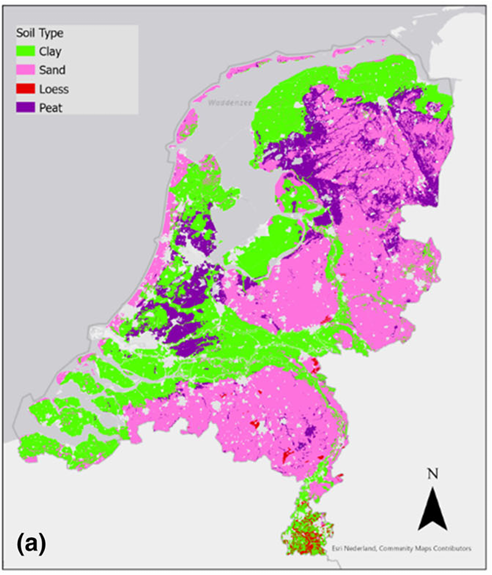
\includegraphics[width=0.5\linewidth]{figures/Soil map bron basisregistratie ondergrond.png}
\caption{National soil classification map of the Netherlands, sourced from the Basisregistratie Ondergrond (BRO).}
\label{fig:soil-type}
\end{figure}


\section{Expert consultation Deltares}


For this thesis, we showed Schasfoort several regions from the dataset during prominent drought periods and asked for her expert opinion on why these impacts might have occurred. This helped us explain and validate the identified drought impacts, while also creating a narrative around the dataset to better understand the underlying causes of the observed events.

For the selected time periods, we focused on the drought of 2022, for which Schasfoort contributed to an expert report for Deltares and was responsible for integrating different perspectives. We also selected the most recent drought event in our dataset, namely 2025. This period was selected because it represents the most recent conditions, meaning that current management practices and system characteristics are likely more comparable to future drought events. Therefore, this period may provide insights that are relevant for understanding future drought impacts.

\begin{figure}[htps!]
    \centering
    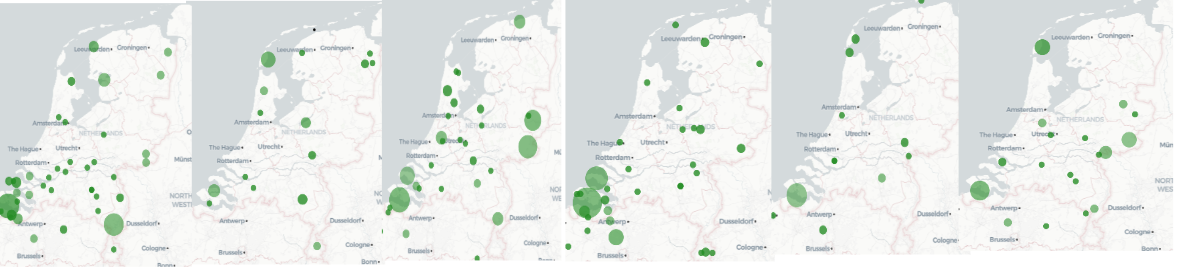
\includegraphics[width=1\linewidth]{figures/Agriculutre 2022 and 2025 may jun jul.png}
    \caption{Agricultural drought impacts reported in newspaper articles in Zeeland during the drought periods of 2022 and 2025 (May--July).}
    \label{fig:agriculture-zeeland}
\end{figure}

When observing the time series of Agricultural drought impacts(Figure~\ref{fig:agriculture-zeeland}), we consistently observe a high number of newspaper reports in Zeeland. These reports contain drought impacts such as: "Driekwart van de boeren in Zeeland heeft echter geen toegang tot zoet water" and "boeren in Zeeland moesten zoetwater aanvoeren met vrachtwagens". According to Femke Schasfoort, this pattern is logical because salinisation is a larger challenge in Zeeland compared to other regions of the Netherlands. The region is highly vulnerable due to its dependence on rainfall as a freshwater source. During drought conditions, freshwater availability becomes limited, and additional measures such as freshwater transport by trucks may be required. Therefore, the observed reporting pattern in our dataset aligns with the expected drought impact mechanisms.

\begin{figure}[htps!]
    \centering
    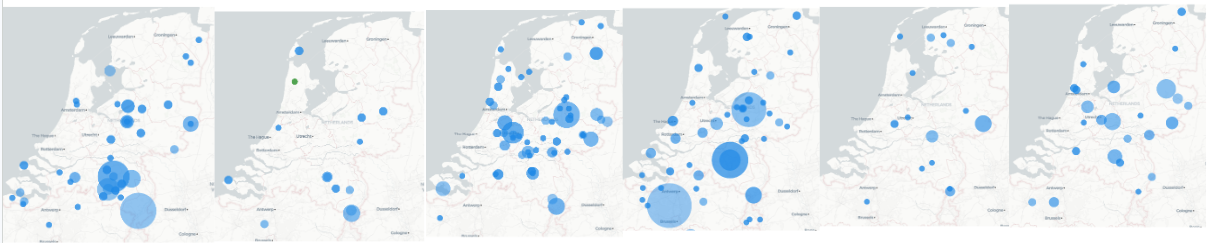
\includegraphics[width=1\linewidth]{figures/Hydrological 2022 and 2025 may jun jul.png}
    \caption{Hydrological drought impacts reported in newspaper articles in Overijssel and Brabant during the drought periods of 2022 and 2025 (May--July).}
    \label{fig:hydrological-overijssel-brabant}
\end{figure}

We also showed Femke a time series of hydrological impacts (Figure~\ref{fig:hydrological-overijssel-brabant}). In Overijssel and Brabant, we observe structurally more newspaper-reported drought impacts compared to other regions. These impacts include groundwater depletion, reservoir and surface water shortages, water use restrictions, and water supply and sanitation issues. Schasfoort explained that the higher impact levels in these regions are related to their physical characteristics. Figure~\ref{fig:soil-type} shows that these areas mainly consist of sandy soils and are relatively elevated compared to other parts of the Netherlands. During droughts or prolonged periods without rainfall, these regions are more difficult to supply with sufficient water. Maintaining freshwater availability requires additional measures, such as pumping water towards elevated areas. Therefore, it is expected that these regions appear as drought impact hotspots in the dataset.

These observations provide validation for the drought impact database. The identified impacts in different domains consistently align with expert knowledge and are supported by logical causal mechanisms.

Schasfoort also mentioned that drought impacts on water-dependent sectors, such as shipping, could provide valuable insights for Deltares. However, after further investigation, we concluded that existing models specifically designed for these applications would likely provide more added value. Schasfoort further highlighted that the ecological consequences of droughts remain a relatively unexplored area for Deltares and governmental agencies. Building upon this observation, we focus the further analysis of the dataset on extracting additional insights into drought impacts on ecological systems, rather than manually investigating individual drought events.


% ==========================================
\part{Impact-Based Forecasting }
\label{part b}
% ==========================================
comment: This part is still heavily under-construction, i do want some feedback on it,  but i do think there is nothing to give feedback on yet. I just left a draft here.


\chapter{Exploratory data analysis}

This section presents an exploratory data analysis (EDA) of the drought impact database. The goal is to understand the characteristics of the dataset before it is used for predictive modelling. In particular, the analysis focuses on identifying temporal, spatial, and thematic patterns that may influence model development and performance.

The section begins with a temporal analysis of yearly trends, seasonality, and their relationship with meteorological drought conditions. Next, the spatial distribution of reported impacts is examined to identify potential geographical biases. Finally, the distribution and co-occurrence of drought impact types are analysed to better understand class imbalance and relationships between impact categories. The findings of this analysis are used to motivate modelling decisions in the following chapter.




\section{Temporal analysis}
\subsection{Volume}

Figure \ref{fig:yearly_volume} shows the yearly number of reported impacts between 2005 and 2025.
From 2005 to 2017, the number of reported impacts remained relatively low, with an average of about 234 impacts per year.
From 2018 onward, the number of reported impacts increased strongly, with an average of about 1,569 impacts per year (12,550 impacts in total; 80.5\% of the 2005--2025 corpus).
The year 2018 corresponds with an extreme drought event in the Netherlands, but the magnitude of the increase suggests that reporting practices may have changed after this period.
\begin{figure}[h!]
    \centering
    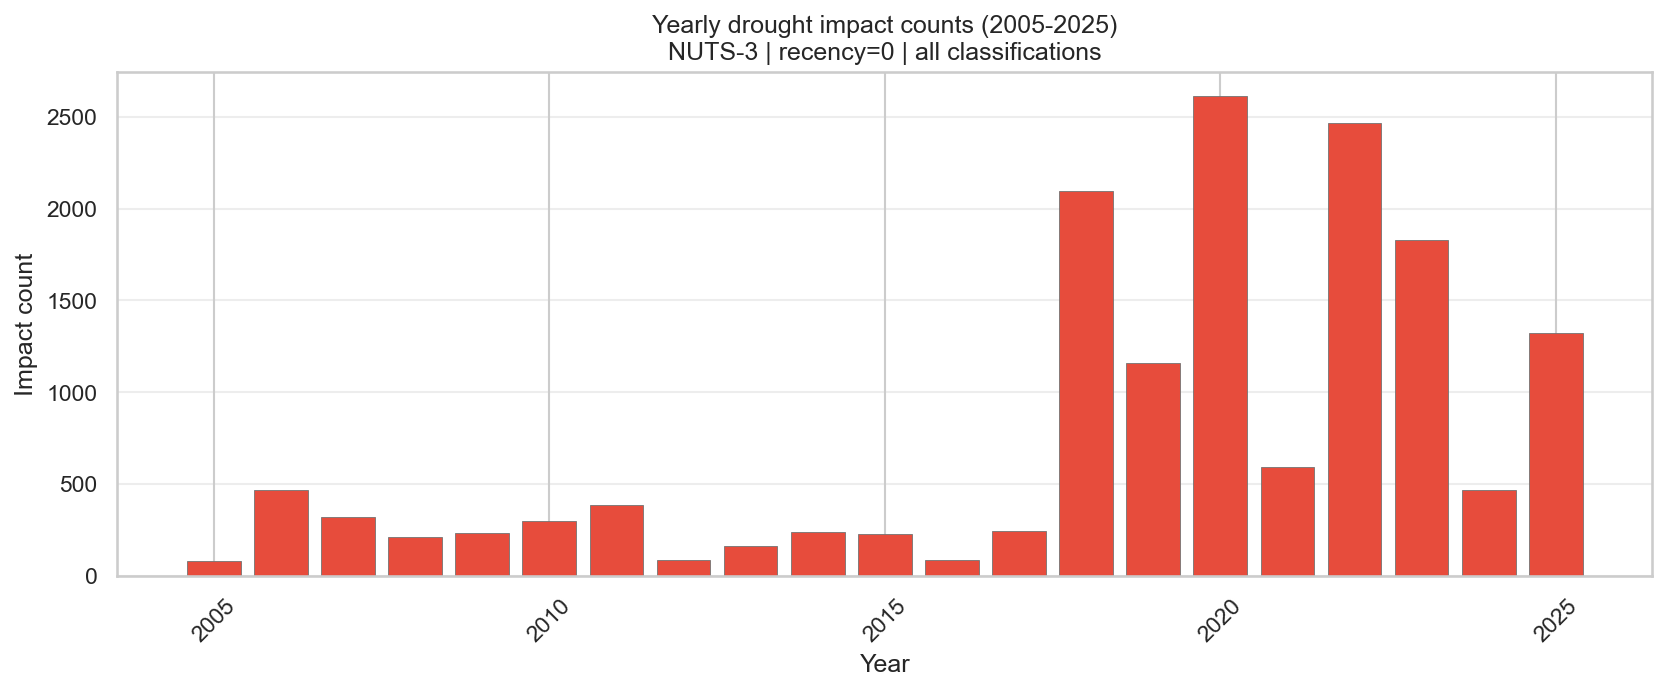
\includegraphics[width=0.98\linewidth]{figures/EDA/fig_yearly_volume.png}
    \caption{Yearly drought impact counts}
    \label{fig:yearly_volume}
\end{figure}
The increase occurred mainly between 2017 and 2018, where the number of reported impacts increased from 244 to 2,095.

Due to this large change, the periods before and after 2018 are treated as separate reporting periods in the remainder of this chapter.

\subsection{Meteorological context}



To provide meteorological context, the yearly number of reported drought impacts is compared with the KNMI national cumulative precipitation deficit on 30 September, a commonly used indicator of drought severity in the Netherlands.

The analysis is performed separately for the two reporting periods (2005--2017 and 2018--2025). Within each period, both the KNMI drought indicator and the yearly number of reported impacts are normalized using min-max scaling. The normalized values are then compared for each year. Years with an absolute difference greater than 0.40 are highlighted, indicating a large mismatch between the reported drought impacts and the meteorological drought indicator.

This threshold-based approach was chosen instead of a correlation coefficient because it is easier to interpret and does not rely on distributional assumptions such as normality.

Figure \ref{fig:meteo_comparision} presents the results. In the period 2005--2017, several years (2007, 2009, 2011, 2013, and 2016) show large differences between the normalized impact counts and the KNMI drought indicator. In contrast, no years exceed the same threshold during the 2018--2025 period.

\begin{figure}
    \centering
    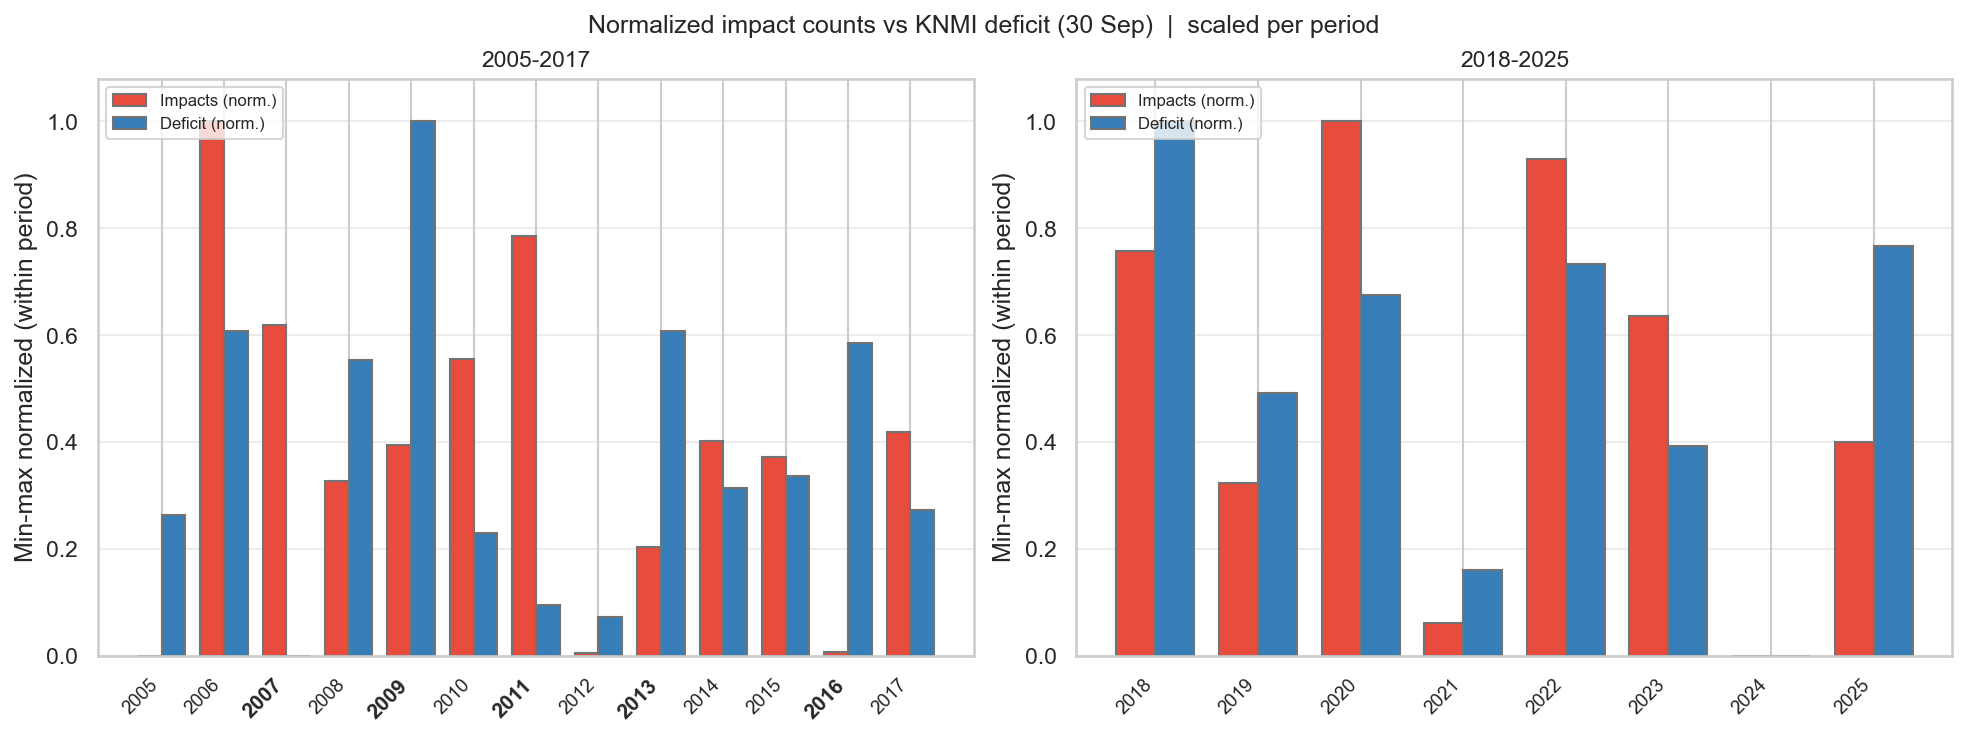
\includegraphics[width=1\linewidth]{figures/EDA/fig_meteo_comparison.png}
    \caption{Bold years mark large within-period mismatches between normalized impacts and KNMI 30-Sep deficit (2007, 2009, 2011, 2013, 2016); no year in 2018–2025 exceeds the same threshold.}
    \label{fig:meteo_comparision}
\end{figure}

These results suggest that the reported drought impacts align more closely with meteorological drought conditions after 2018 than before. For the pre-2018 period, the extracted news signal appears to be weaker and less consistent with the observed drought conditions. This does not imply that individual drought impacts or sectors cannot be modelled during this period. Instead, it suggests that the overall reporting signal is relatively weak, making it more difficult to distinguish years with different levels of drought severity.

One possible explanation is that drought impacts in the news were reported less consistently before 2018, resulting in a dataset with a lower signal-to-noise ratio. Consequently, the pre-2018 data should be interpreted with caution when used for predictive modelling. For this reason, the models developed in this thesis primarily focus on the 2018--2025 period, where the relationship between reported impacts and meteorological drought conditions appears to be more consistent.


\subsection{Monthly seasonality}

When aggregating impact mentions by publication month, a strong seasonal pattern is observed. Approximately 61\% of all impact mentions are published between May and September, while July and August together account for around one-third of the complete dataset. In contrast, the winter months December, January, and February together contain only around 13\% of all mentions. Figure \ref{fig:seasonality} shows this seasonality.

\begin{figure}
    \centering
    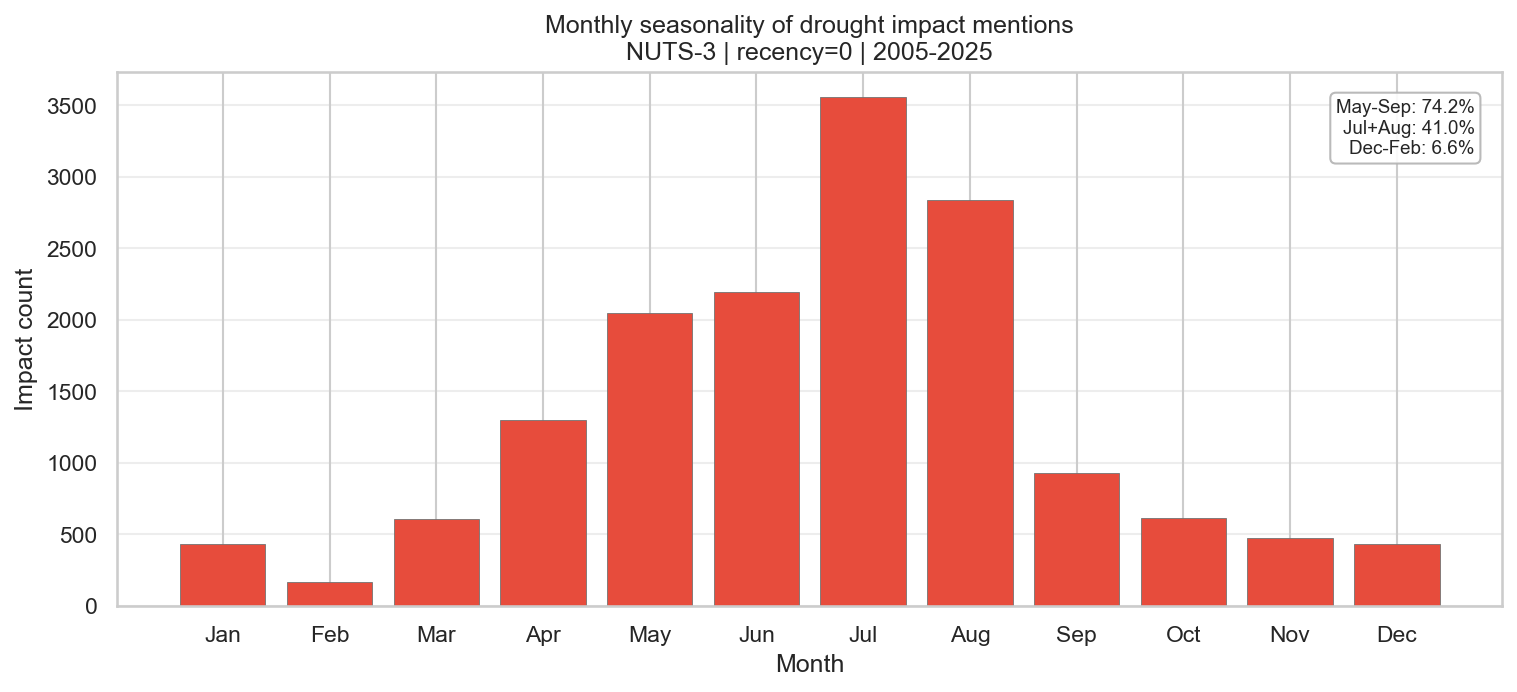
\includegraphics[width=1\linewidth]{figures/EDA/fig_monthly_seasonality.png}
    \caption{Monthly seasonality Drought impacts}
    \label{fig:seasonality}
\end{figure}

This seasonal pattern is partly consistent with drought processes, as summer conditions are associated with higher temperatures, increased evaporation, and greater water stress. However, the strong concentration of reports during summer may also indicate a reporting bias, where drought impacts are more frequently reported when they are more visible and receive more public attention.





\section{Spatial analysis}

Figure~\ref{fig:choropleth-nuts3} shows that a higher number of reported impacts is observed in regions with sandy soils. The five NUTS-3 regions with the highest reported impact totals are Achterhoek (797), Veluwe (715), Zuidoost-Noord-Brabant (709) and West-Noord-Brabant (592). These regions are characterised by intensive agriculture, sandy soils, and relatively shallow groundwater levels. Overig Zeeland (616) has high impacts because it mainly depends on rain water.

\begin{figure}[h!]
    \centering
    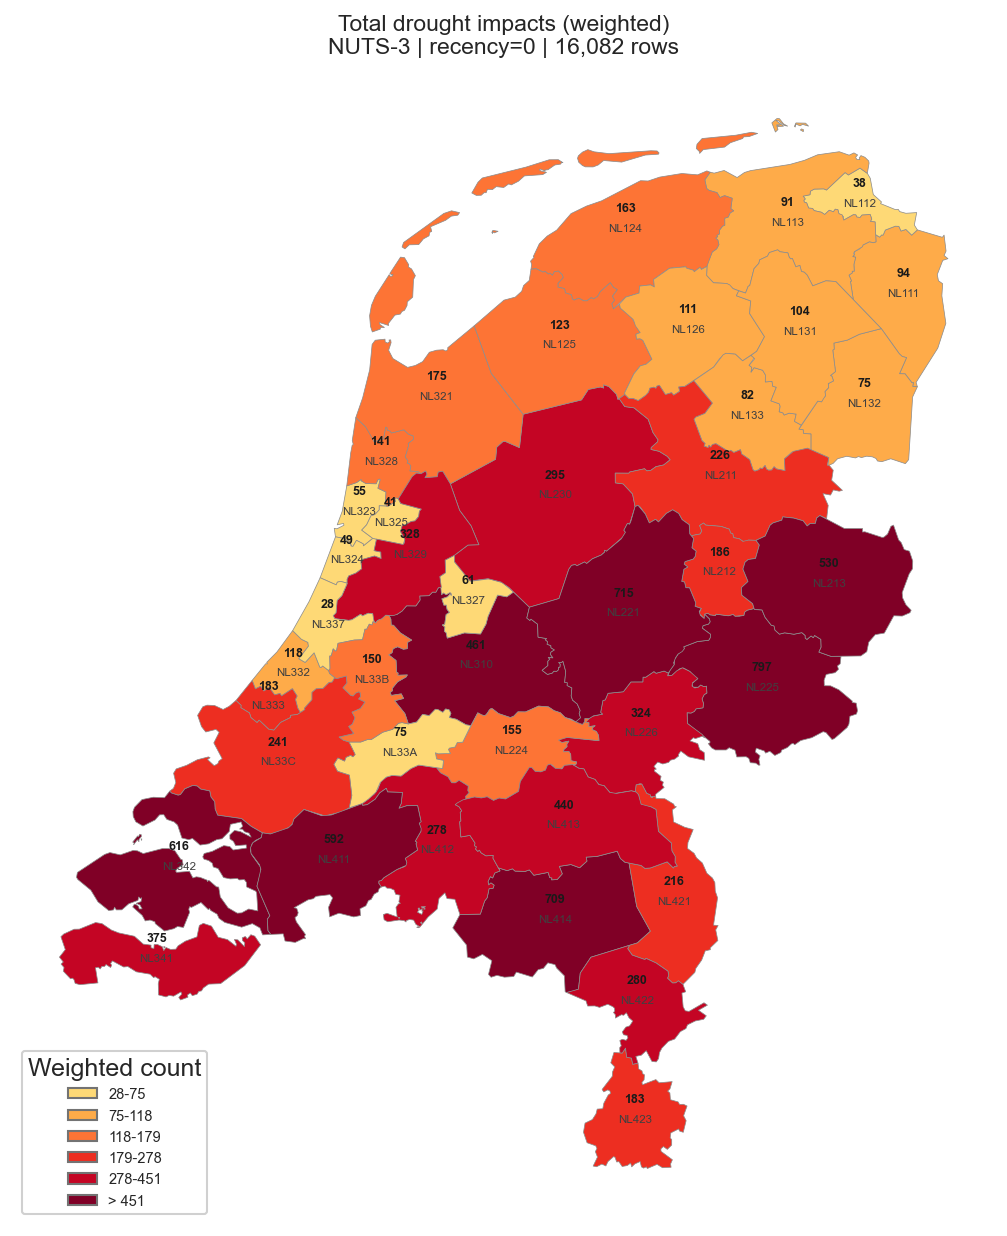
\includegraphics[width=0.5\linewidth]{figures/EDA/fig_choropleth_nuts3.png}
    \caption{Total weighted drought impact counts by NUTS-3 region (2005--2025; \texttt{recency\_in\_months}=0). Darker colours indicate higher impact totals; values shown on the map are region totals.}
    \label{fig:choropleth-nuts3}
\end{figure}

The lowest impact totals occur mainly in densely populated urban regions of the Randstad, such as Agglomeratie Leiden en Bollenstreek (28), Zaanstreek (41), and Agglomeratie Haarlem (49). Since these regions are not characterised by low population density, the spatial distribution of reported drought impacts appears to be more strongly related to land use and hydrogeological conditions than to population density or media presence.

This suggests that variables such as population density, which are commonly used in drought impact studies at coarser spatial resolutions, may have limited explanatory power for this dataset. Instead, land use and hydrological characteristics may be more relevant predictors of drought impacts in the Netherlands.

Additionally, the specific geographical characteristics of the Netherlands should be considered. A large part of the country is located below sea level, meaning that elevation and water management systems may influence drought vulnerability. For example, maintaining groundwater levels in elevated sandy regions can be more challenging than in lower-lying areas where water can be supplied more easily through existing infrastructure.

Based on these observations, the selection of model input variables should consider the specific Dutch context. Variables related to land use, soil type, groundwater availability, and elevation may provide more relevant information for drought impact modelling than variables commonly applied in other regions.

\section{Impact characteristic's}

\subsubsection{Sector distribution}

Grouping the 19 impact classifications into their six thematic categories
gives the following weighted distribution: agriculture 5,093 (36.2\%),
water 4,253 (30.2\%), ecosystem 2,450 (17.4\%), fire/heat 1,307 (9.3\%),
economy 522 (3.7\%), and social 460 (3.3\%). Agriculture and water together
account for two-thirds of all reported impacts. The overall sector distribution is shown in Figure \ref{fig:class_distribution}, representing a highly imbalanced dataset across sectors.

\begin{figure}[h!]
    \centering
    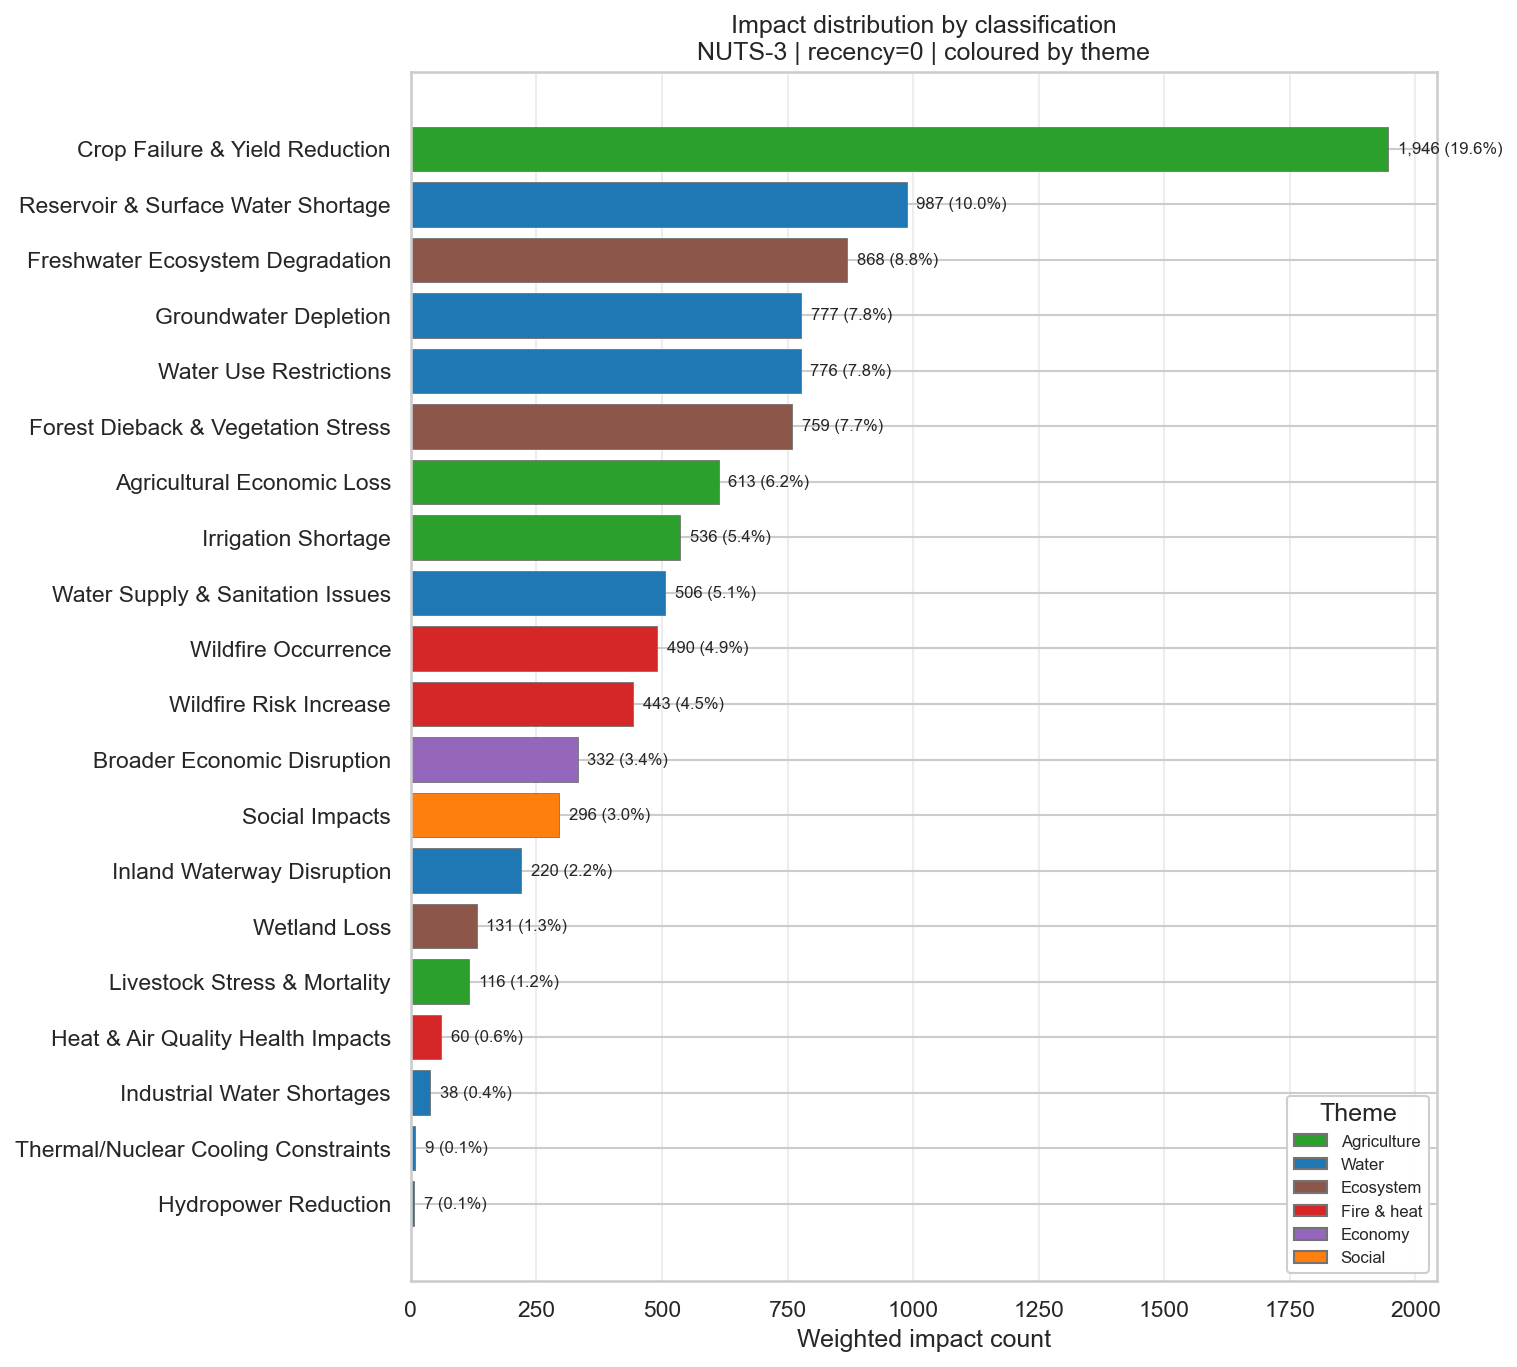
\includegraphics[width=0.85\linewidth]{figures/EDA/fig_class_distribution.png}
    \caption{The distribution of drought impact across all 19 classes.}
    \label{fig:class_distribution}
\end{figure}

\subsection{Co-occurrence signals}

Some impacts frequently co-occur and are often reported together. In this analysis, impact co-occurrence is defined as impacts that co-occur \textbf{within the same news-article}. Co-occurrence patterns in this dataset can be caused by the following mechanism.  Impacts are connected through underlying causal chains. For example, a reduction in crop yield can lead to agricultural economic losses.

Figure \ref{fig:cooccurrence_article_arc} shows the co-occurrence patterns between different impact types. From these patterns, several potential impact chains can be identified:

\begin{figure}
    \centering
    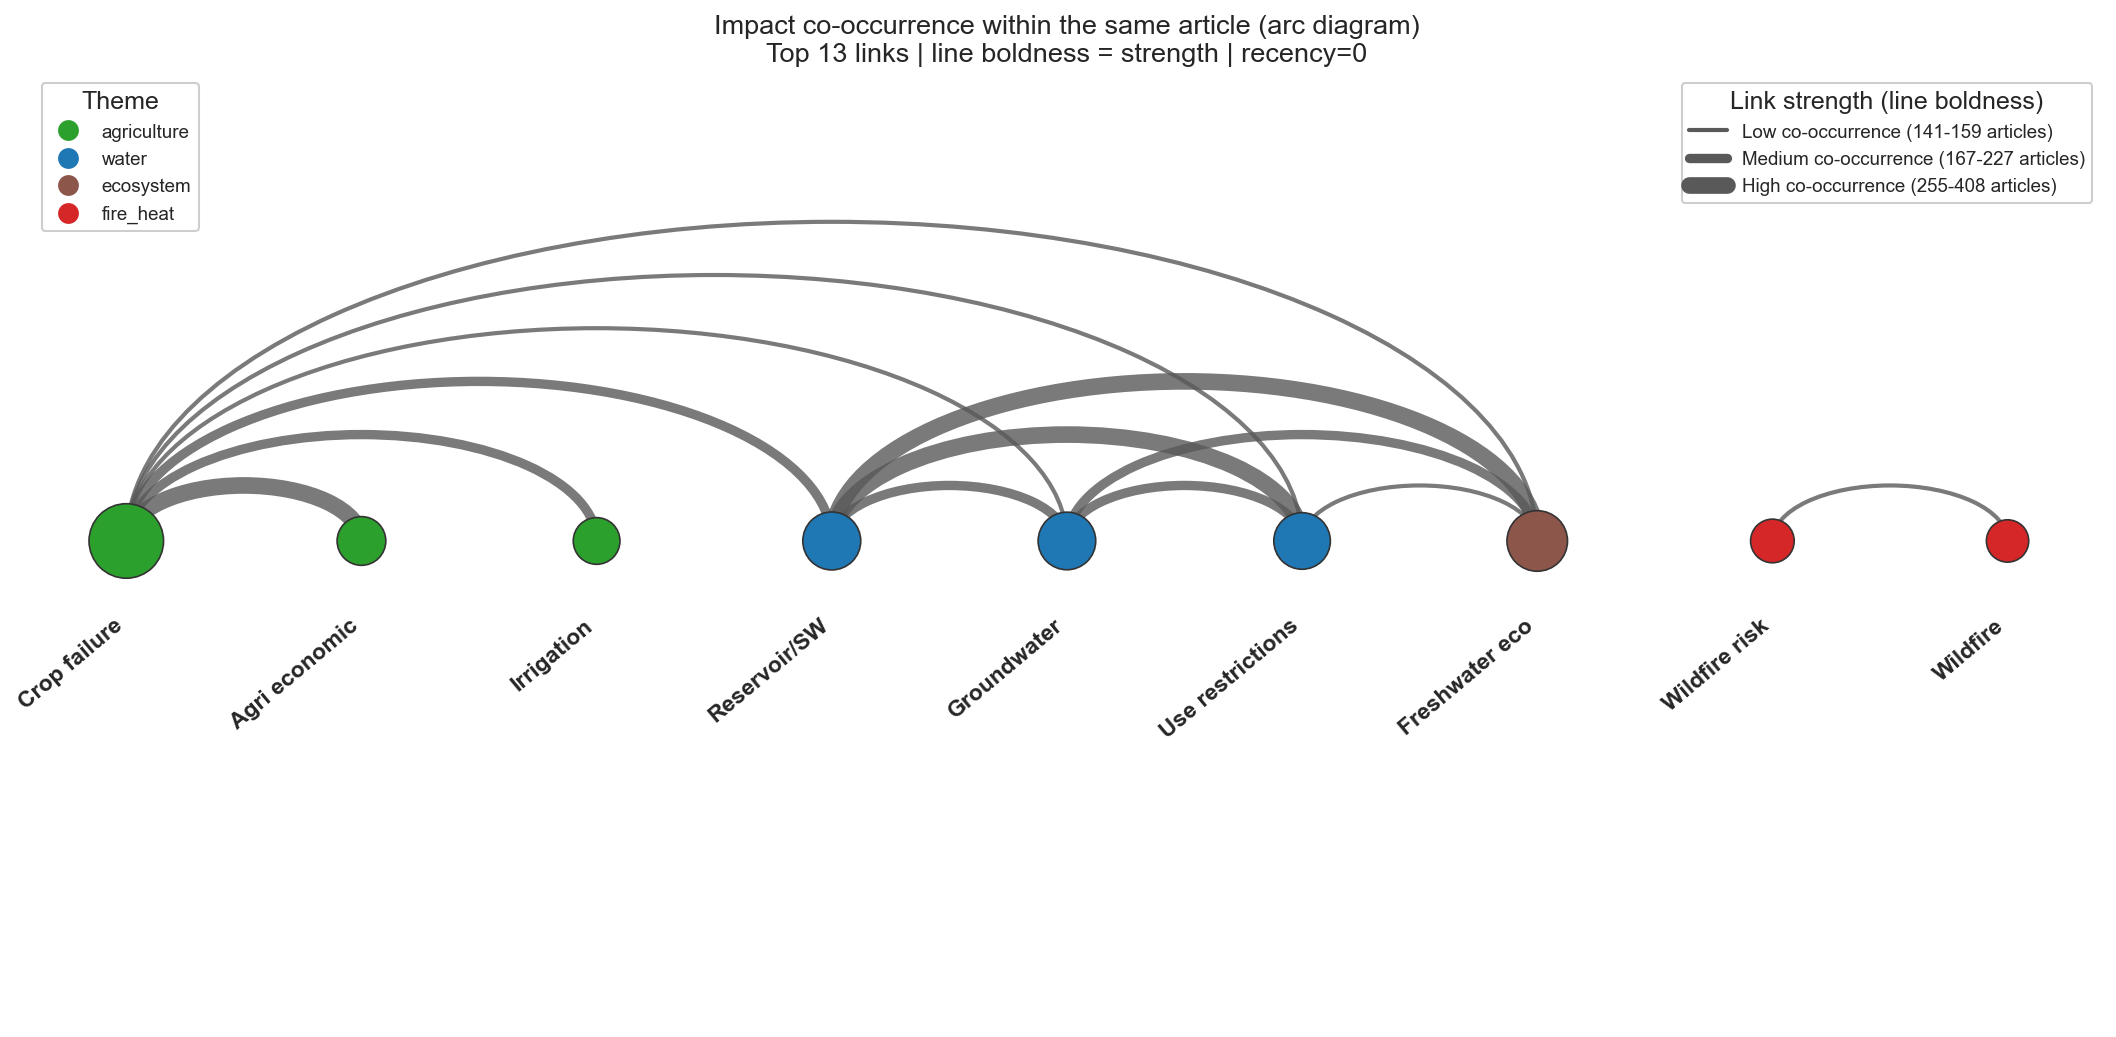
\includegraphics[width=1\linewidth]{figures/EDA/fig_cooccurrence_article_arc.png}
    \caption{Co-occurrence of top 13 impact links}
    \label{fig:cooccurrence_article_arc}
\end{figure}

\begin{itemize}
    \item Wildfire risk increase $\rightarrow$ wildfire occurrence
    \item Irrigation shortage $\rightarrow$ crop yield loss $\rightarrow$ agricultural economic loss
    \item Surface water shortage / groundwater shortage $\rightarrow$ water use restrictions / freshwater ecosystem degradation
\end{itemize}

These co-occurrence signals suggest that drought impacts are not independent events but can form connected chains. This information could potentially be used to simplify the modelling problem in several ways.

One option is to predict complete impact chains instead of individual impact classes. In this approach, an impact chain would become the prediction target rather than a single impact type. A second option is to focus on the beginning of these chains and model the occurrence of key initiating impacts, such as irrigation shortages, wildfire risk increases, or surface water shortages.

A third possibility is to focus on the relationships between impacts rather than predicting impacts directly. For example, instead of predicting when a water shortage occurs, a model could predict under which conditions a water shortage leads to water use restrictions. This would shift the modelling approach from predicting impacts towards modelling the links between impacts.

However, this type of causal impact modelling is likely already addressed in more specialised domain models developed for specific applications. A potential research direction inspired by the observed co-occurrence patterns is the use of Bayesian networks, which can explicitly represent relationships between variables and causal dependencies. This could provide an alternative to more commonly used machine learning approaches, within IBF such as random forests, which primarily model statistical relationships without explicitly representing causal structures. An other potential research venue could be using an causal random forest model, where we add causal rules to our random forest model.

\section{Implications for predictive modelling}

The exploratory data analysis highlights several characteristics of the drought impact database that should be considered during model development.

First, the temporal analysis identified a clear distribution shift after 2018. The stronger relationship between reported impacts and meteorological drought conditions suggests that the period 2018--2025 provides a more consistent training dataset than the earlier years. As a result, the predictive models developed in this thesis focus primarily on this period.

Second, the spatial analysis indicates that reported impacts are concentrated in agricultural regions with sandy soils. This suggests that variables describing land use, soil type, groundwater conditions, and elevation are likely to be more informative than population-based variables alone. The Dutch landscape differs from many previous drought impact studies, so feature selection should account for these regional characteristics.

Third, the impact distribution is highly imbalanced, with agriculture and water-related impacts dominating the dataset. This class imbalance should be considered during both model training and evaluation, as models may otherwise favour the largest classes.

Finally, the co-occurrence analysis shows that drought impacts sometimes occur in connected impact chains rather than as isolated events. Although this thesis predicts individual impact classes, these relationships suggest several directions for future work, including modelling impact chains directly or using causal machine learning methods such as Bayesian networks or causal random forests.

Together, these findings provide the basis for the feature selection and modelling choices described in the next chapter.



% This has to do with the underlying impact signals, but also with the way the llmn extract's the data. In our current str


% Some impacts co-occur alot, and some specif impcats do not co-occur alot. This has to do with the underlying procces in the impacts themeselves. To validate the database, and construct sort of an impact chain graph using network anlysis, we can create impact chains, to validate and visuliaze how the data is co-occuring alot. 

% The first step is to build an co-occurence matrix, what impact's co-occur alot, and how often do they co-occur. The question we want to anwser what drought impact do often co-occur together, and in what dirrection do they corruc? Then we have to add another constrained we want to make an directed graph, so that we can sort of visuliaze what impact's, lead to other impacts. 



% Building upon impact chan theory described in Section \ref{sec:impact_chain_theory}. 

















% ----------------------------

% \section{Research outputs: profiling the drought impact database}
% \label{sec:research-outputs}

% \subsection{Database overview}
% \label{subsec:db-overview}

% The database underlying this thesis is built from Dutch news articles
% processed by an LLM extraction pipeline, which identifies individual
% drought-impact mentions and assigns each one a location, an impact
% classification, a severity score, and a confidence score. Because a single
% article frequently reports several distinct impacts (e.g. a article about
% low river levels may simultaneously mention shipping disruption, water
% quality problems, and drinking-water concerns), it is important to
% distinguish two different units of analysis throughout this chapter:
% \emph{articles} (source documents) and \emph{impact mentions} (individual
% extracted impact statements, the unit the classifier is ultimately trained
% on).

% The full extraction output contains 48,444 impact mentions drawn from
% 15,318 unique articles (an average of 3.16 impact mentions per article),
% published between August 2004 and June 2026. Of these mentions, 22,658
% (46.8\%) could be geocoded precisely to one of the 40 Dutch NUTS-3 regions;
% the remainder refer to locations outside the Netherlands (32.3\%), resolve
% only to the country level (8.9\%), or could not be geocoded at all (12.0\%).
% This chapter focuses on the NUTS-3-resolvable subset, which spans 6,489
% unique articles and covers all 40 NUTS-3 regions and all 12 NUTS-2 provinces
% in the Netherlands. Within this subset, the average article mentions 1.85
% distinct impact classifications, and just over half of all articles
% (52.5\%) report more than one type of impact --- an early indication that
% drought impacts are rarely reported in isolation (see
% Section~\ref{subsec:impact-characteristics}).

% Impacts are grouped into 19 fine-grained classifications spanning six
% thematic groups: agriculture, water, ecosystem, fire/heat, economy, and
% social. Table~\ref{tab:db-overview} summarises the key scope statistics for
% the NUTS-3 subset used throughout the remainder of this chapter.

% \begin{table}[htbp]
%     \centering
%     \caption{Scope of the drought impact database (NUTS-3-resolvable subset).}
%     \label{tab:db-overview}
%     \begin{tabular}{lr}
%         \toprule
%         Quantity & Value \\
%         \midrule
%         Impact mentions (rows) & 22{,}658 \\
%         Unique source articles & 6{,}489 \\
%         Weighted impact count (mention-weighted) & 14{,}085 \\
%         Time period covered & 2004--2026 (bulk: 2005--2025) \\
%         NUTS-3 regions represented & 40 / 40 \\
%         NUTS-2 provinces represented & 12 / 12 \\
%         Impact classifications & 19 (6 thematic groups) \\
%         Articles reporting $>1$ impact type & 52.5\% \\
%         \bottomrule
%     \end{tabular}
% \end{table}

% \subsection{Temporal analysis}
% \label{subsec:temporal-analysis}

% \subsubsection{Yearly trends}

% \begin{figure}[htbp]
%     \centering
%     \includegraphics[width=0.85\textwidth]{images for report 2/bar_total_impacts_over_time.png}
%     \caption{Total reported drought impacts per year, 2005--2025.}
%     \label{fig:yearly-trend}
% \end{figure}

% Figure~\ref{fig:yearly-trend} shows annual impact counts restricted to
% 2005--2025. Between 2005 and 2017, yearly totals fluctuate between 121 and
% 578 (mean $\approx$ 325/year, total 4,227 impacts). From 2018 onward, annual
% totals jump to the low thousands (total 17,842 impacts over 2018--2025,
% mean $\approx$ 2,230/year) --- a step-change of roughly 4.2x in the average
% reporting rate, occurring almost entirely within a single year (2017: 376
% $\rightarrow$ 2018: 3,333). This shape --- an abrupt jump rather than a
% gradual ramp --- is the basis for treating 2005--2017 and 2018--2025 as two
% distinct reporting regimes for the remainder of this chapter.

% \subsubsection{Monthly seasonality}

% Aggregating impact mentions by publication month (full corpus, all
% geocoding levels) reveals a strong seasonal signal: 61\% of all impact
% mentions are published between May and September, with July (8,398
% mentions) and August (7,328) alone accounting for over a third of the
% entire corpus. The winter months are comparatively quiet: December,
% January, and February together account for only 13.5\% of mentions.
% \emph{[Figure to add: monthly histogram of impact mentions, currently not
% in the notebook --- can be generated from \texttt{publication\_date.dt.month}
% grouped counts.]}

% This pattern is only partly explained by actual drought physics. Summer is
% indeed when soil-moisture deficits, low river levels, and visible crop
% stress peak in the Netherlands, so some seasonality is expected. But the
% sharpness of the July/August spike also reflects a media-attention effect:
% drought is most newsworthy when it is visually and physically salient (heat,
% visible crop damage, low water levels for recreation), whereas slower-onset
% impacts such as groundwater depletion or ecosystem stress that persist into
% autumn and winter are comparatively under-reported once the summer news
% cycle ends. This is a second, independent reporting bias --- distinct from
% the year-level step-change --- that should be considered when interpreting
% month-level patterns in the data.

% \subsubsection{Relation to major drought years}

% The years with the highest impact counts in the post-2018 regime --- 2018,
% 2020, and 2022 --- correspond to the years widely documented as the most
% severe recent Dutch droughts, all part of the well-known cluster of dry
% summers between 2018 and 2022. This qualitative alignment is quantified
% formally in Section~\ref{subsec:meteo-context}.

% \subsubsection{Discussion of reporting bias}

% Taken together, the yearly and monthly patterns above indicate that the
% database's temporal structure is shaped as much by \emph{when and how
% drought gets reported} as by the underlying meteorological signal. The
% 2018 step-change most plausibly reflects a genuine shift in reporting
% volume/consistency (e.g. broader media and institutional attention
% following the record 2018 drought) rather than a sixfold increase in actual
% drought incidence in a single year. Similarly, the summer concentration of
% reports reflects newsworthiness as much as it reflects the physical timing
% of drought onset. Both biases matter directly for later chapters: any
% model trained on raw report volume as a proxy for drought intensity is, in
% part, learning a media-attention signal.

% \subsection{Spatial analysis}
% \label{subsec:spatial-analysis}

% \subsubsection{NUTS-2 / NUTS-3 maps}

% \begin{figure}[htbp]
%     \centering
%     
\includegraphics[width=0.85\textwidth]{outputs/eda_heatmaps/choropleth_total_impacts.png}
%     \caption{Total reported drought impacts per NUTS-3 region (weighted counts).}
%     \label{fig:choropleth-nuts3}
% \end{figure}

% At NUTS-3 resolution (Figure~\ref{fig:choropleth-nuts3}), impact reporting
% is concentrated in a relatively small number of regions. At the coarser
% NUTS-2 level, the concentration is still visible: three provinces ---
% Gelderland (2,660 weighted impacts), Noord-Brabant (2,656), and Overijssel
% (1,542) --- together account for 48.7\% of all weighted impacts, despite
% being only 3 of the Netherlands' 12 NUTS-2 provinces.
% \emph{[Figure to add: a NUTS-2 choropleth analogous to
% Figure~\ref{fig:choropleth-nuts3}, aggregating the existing NUTS-3 output up
% one administrative level --- not yet generated in the notebook.]}

% \subsubsection{Regional hotspots}

% The five NUTS-3 regions with the highest reported impact totals are
% Achterhoek (1,067), Veluwe (973), Zuidoost-Noord-Brabant (930), Overig
% Zeeland (928), and Twente (812) --- all agriculturally intensive areas on
% sandy soils with shallow groundwater tables. The lowest totals occur in
% dense, urbanised parts of the Randstad: Agglomeratie Leiden en
% Bollenstreek (43), Zaanstreek (53), and IJmond (70). Since these low-count
% regions are not low-population --- if anything the opposite --- the spatial
% pattern looks like a land-use/hydrogeology signal rather than a
% population- or media-density signal.

% \subsubsection{Density of impacts}

% The counts and maps above are absolute totals, not normalised by region
% size or population, so they should not yet be read as "risk density." A
% fair density comparison would divide each region's weighted impact count by
% its agricultural area (to test the land-use hypothesis) and, separately, by
% its population (to test whether the low urban counts genuinely reflect a
% reporting gap rather than a lower urban exposure to drought).
% \emph{[Analysis to add: per-km\textsuperscript{2} and per-capita normalised
% choropleths --- requires joining NUTS-3 area/population figures, e.g. from
% CBS or Eurostat, not currently in the notebook.]} Until this is done, the
% "hotspot" language in this section should be understood as a statement
% about reporting volume, not confirmed drought risk density.

% \subsection{Impact characteristics}
% \label{subsec:impact-characteristics}

% \subsubsection{Sector distribution}

% Grouping the 19 impact classifications into their six thematic categories
% gives the following weighted distribution: agriculture 5,093 (36.2\%),
% water 4,253 (30.2\%), ecosystem 2,450 (17.4\%), fire/heat 1,307 (9.3\%),
% economy 522 (3.7\%), and social 460 (3.3\%). Agriculture and water together
% account for two-thirds of all reported impacts, consistent with the
% regional pattern in Section~\ref{subsec:spatial-analysis}: both the
% sectoral mix and the spatial hotspots point toward the same underlying
% driver, namely agriculturally exposed, sandy-soil regions.

% \subsubsection{Cascading impacts and impact chains}

% Because 52.5\% of articles report more than one impact type, it is possible
% to treat co-occurring classifications within the same article as a proxy
% for cascading impact chains. Table~\ref{tab:cooccurrence} lists the most
% frequently co-occurring classification pairs within a single article.

% \begin{table}[htbp]
%     \centering
%     \caption{Most frequent co-occurring impact-classification pairs within the same article (NUTS-3 subset, $n=6{,}489$ articles).}
%     \label{tab:cooccurrence}
%     \begin{tabular}{lr}
%         \toprule
%         Co-occurring pair & Articles \\
%         \midrule
%         Agricultural Economic Loss $\leftrightarrow$ Crop Failure \& Yield Reduction & 661 \\
%         Freshwater Ecosystem Degradation $\leftrightarrow$ Reservoir \& Surface Water Shortage & 358 \\
%         Crop Failure \& Yield Reduction $\leftrightarrow$ Irrigation Shortage & 325 \\
%         Reservoir \& Surface Water Shortage $\leftrightarrow$ Water Use Restrictions & 290 \\
%         Freshwater Ecosystem Degradation $\leftrightarrow$ Groundwater Depletion & 289 \\
%         Groundwater Depletion $\leftrightarrow$ Reservoir \& Surface Water Shortage & 240 \\
%         Crop Failure \& Yield Reduction $\leftrightarrow$ Groundwater Depletion & 214 \\
%         Groundwater Depletion $\leftrightarrow$ Water Use Restrictions & 207 \\
%         Wildfire Occurrence $\leftrightarrow$ Wildfire Risk Increase & 180 \\
%         \bottomrule
%     \end{tabular}
% \end{table}

% Two distinct chains emerge from this table. The first is an
% agricultural chain: \emph{Crop Failure} co-occurs strongly with
% \emph{Irrigation Shortage} and \emph{Agricultural Economic Loss}, tracing a
% direct physical impact through to its economic consequence. The second is a
% water-system chain: \emph{Groundwater Depletion}, \emph{Reservoir \&
% Surface Water Shortage}, \emph{Freshwater Ecosystem Degradation}, and
% \emph{Water Use Restrictions} form a tightly interconnected cluster,
% consistent with a single hydrological cause propagating through surface
% water, groundwater, ecosystems, and policy response almost simultaneously
% within the same article. \emph{[Figure to add: a co-occurrence heatmap or
% network diagram of the full classification pair-count matrix would make
% this pattern easier to read than the table above.]}

% \subsubsection{Direct versus indirect impacts}

% Using the thematic grouping as a rough proxy --- treating economy and
% social impacts as downstream/indirect consequences, and
% agriculture/water/ecosystem/fire-heat impacts as direct physical
% consequences --- indirect impacts make up only 7.0\% of weighted mentions
% (982 of 14,085), against 93.0\% direct. This imbalance is worth stating
% explicitly: the database is overwhelmingly composed of \emph{direct}
% physical drought impacts, and the economic and social consequences of
% drought are comparatively rarely captured as a distinct, separately
% reported category, even though the co-occurrence analysis above shows they
% are frequently mentioned alongside a direct impact in the same article.

% \subsection{Meteorological context}
% \label{subsec:meteo-context}

% \begin{figure}[htbp]
%     \centering
%     \includegraphics[width=\textwidth]{images for report 3/timeseries_total_impacts.png}
%     \caption{Yearly impact counts versus KNMI cumulative precipitation deficit (30 September), shown separately per reporting regime with independent scaling.}
%     \label{fig:meteo-comparison}
% \end{figure}

% To test whether reported impact volume tracks actual meteorological drought
% severity, yearly impact counts (2005--2025) were compared against the KNMI
% national cumulative precipitation deficit as of 30 September --- a standard
% Dutch drought-severity indicator. The relationship differs sharply between
% the two reporting regimes identified in
% Section~\ref{subsec:temporal-analysis}:

% \begin{itemize}
%     \item \textbf{2005--2017:} Pearson $r = -0.02$ ($p = 0.87$), Spearman
%     $\rho = -0.05$ ($p = 0.87$) --- no detectable relationship between
%     yearly impact counts and the deficit.
%     \item \textbf{2018--2025:} Pearson $r = 0.78$ on raw counts (log-scaled:
%     $r = 0.84$, $p = 0.01$), Spearman $\rho = 0.60$ ($p = 0.12$) --- a
%     clear positive relationship, though the sample is small ($n=8$ years)
%     and statistical power is limited.
% \end{itemize}

% This is a striking result: reported impact volume is essentially unrelated
% to physical drought severity before 2018, but becomes a reasonably good
% proxy for it afterward. This is consistent with the reporting-regime
% interpretation from Section~\ref{subsec:temporal-analysis} --- before 2018,
% reporting was too sparse and inconsistent for its year-to-year variation to
% reflect real conditions; from 2018 onward, with a larger and more
% consistent volume of reporting, the aggregate signal starts to behave like
% a genuine (if noisy) drought indicator. A practical implication is that the
% pre-2018 subset should not be relied upon as ground truth for drought
% severity, while the post-2018 subset can be used with more confidence,
% subject to the caveats below.

% \subsubsection{Lead/lag relationships}

% A simple one-year-lag check (this year's impact count against last year's
% deficit) across the full 2005--2025 series gives $r = 0.23$ --- weak, and
% likely dominated by the level shift between regimes rather than a genuine
% lag effect. A within-regime lag analysis (particularly for 2018--2025) would
% require more years of data than are currently available to be conclusive,
% and should be revisited once more years accumulate.

% \subsubsection{Other meteorological variables}

% This comparison currently uses only the KNMI 30-September cumulative
% deficit. The processed meteorological dataset
% (\texttt{meteo\_nuts3\_monthly.parquet}, Chapter~7) also contains monthly
% SPEI-12 and, potentially, groundwater/soil-moisture fields at NUTS-3
% resolution, which would allow the comparison in this section to be repeated
% at regional rather than national level. \emph{[Analysis to add: NUTS-3-level
% correlation between weighted impact counts and local SPEI-12/groundwater
% anomalies, to test whether the national-level correlation above also holds
% regionally, or whether it is driven by a handful of high-volume regions.]}

% \subsection{Implications for predictive modelling}
% \label{subsec:modelling-implications}

% The patterns documented in this chapter translate into five concrete
% constraints that should inform how this database is used as training data
% in later chapters:

% \begin{enumerate}
%     \item \textbf{Temporal imbalance.} 79\% of all NUTS-3-resolvable impact
%     mentions (17,842 of 22,658) fall in 2018--2025, against 21\% in
%     2005--2017. Any temporal split or cross-validation scheme must account
%     for this, e.g. by stratifying by period rather than by simple random
%     year holdout.
%     \item \textbf{Spatial imbalance.} Just three NUTS-2 provinces account
%     for 48.7\% of weighted impacts, and the lowest-reporting NUTS-3 regions
%     have roughly 25x fewer impacts than the highest. A model evaluated only
%     on aggregate accuracy will be dominated by performance in a handful of
%     agricultural regions.
%     \item \textbf{Class imbalance.} The largest classification (\emph{Crop
%     Failure \& Yield Reduction}, 4,696 raw mentions) outweighs the smallest
%     (\emph{Hydropower Reduction}, 11 mentions) by roughly two orders of
%     magnitude, requiring explicit handling via class weighting,
%     oversampling, or per-class rather than aggregate evaluation metrics.
%     \item \textbf{Reporting bias.} Reported volume is not a stable proxy for
%     drought severity: it correlates with the KNMI deficit only in the
%     post-2018 regime ($r=0.78$) and not before ($r=-0.02$), and is further
%     biased toward the summer months regardless of when the underlying
%     drought conditions actually developed.
%     \item \textbf{Data sparsity and geocoding precision.} Only 46.8\% of all
%     extracted impact mentions could be geocoded to NUTS-3 precision; the
%     rest are foreign-location mentions (32.3\%), country-level-only matches
%     (8.9\%), or ungeocodable (12.0\%). This is itself a form of sparsity
%     that limits how much of the raw corpus is usable for a location
%     classifier, independent of the temporal and spatial imbalances above.
% \end{enumerate}




























% -1. Seasonality

% 0. Imbalanced data

% --- Classes

% --- Temporal coverage

% --- Spatial hotspots.


% 1. Correlation's with meto variable's. 


% 3. Correlations with meteo variable's




% ----> litature inspired baseline.

% ----> well thought out model


% --> speciy attribution model










\chapter{Baseline Drought Impact Forecasting Model}


\section{Prediction problem formulation}

Based on the literature review in Chapter 2, the system requirements defined in Chapter 3, the database validation in Chapter 7, and the exploratory data analysis presented in the previous chapter, the machine learning prediction problem can now be formally defined. Earlier chapters established the limitations of existing impact-based forecasting systems and identified the characteristics of the constructed drought impact database. These findings are used to define the spatial scale, forecasting horizon, and impact categories considered in the prediction task.

The objective is to predict the occurrence of multiple drought impacts for a given region and future time period. Each observation consists of a region $r$ at time $t$, represented by a feature vector:

\begin{equation}
\mathbf{x}_{r,t} =
[x_1,x_2,\ldots,x_p],
\end{equation} where $p$ represents the number of predictor variables describing the state of the region at time $t$. The prediction target is represented as a multi-label vector:

\begin{equation}
\mathbf{y}_{r,t+h} =
[y_1,y_2,\ldots,y_K],
\end{equation} where $K$ represents the number of impact classes considered in the prediction framework. Each element of the vector is defined as:

\begin{equation}
y_k =
\begin{cases}
1, & \text{if impact class } k \text{ occurs in region } r \text{ at time } t+h,\\
0, & \text{otherwise.}
\end{cases}
\end{equation} The objective of the machine learning model is to estimate future drought impact occurrences based on the available predictor variables. This can be formulated as:

\begin{equation}
\hat{\mathbf{y}}_{r,t+h}=f(\mathbf{x}_{r,t}),
\end{equation} where $f$ represents the trained machine learning model, $\mathbf{x}_{r,t}$ represents the predictor variables describing region $r$ at time $t$, and $\hat{\mathbf{y}}_{r,t+h}$ represents the predicted impact occurrence vector for region $r$ at lead time $h$.



In this thesis, the general formulation above is specified based on the limitations and opportunities identified in previous chapters. The spatial unit $r$ is defined at the NUTS-3 regional level. This choice addresses a limitation identified in previous impact-based forecasting studies, where predictions were often performed at larger spatial scales, such as national, NUTS-1, or provincial levels. Although these larger spatial units reduce prediction difficulty by aggregating local variability, they provide limited information for regional decision making.

The forecasting horizon $h$ is defined as zero to three months, with particular focus on one-month-ahead predictions. This choice follows findings from previous studies, which indicate that predictive skill generally decreases as lead times increase and approaches random performance at longer forecasting horizons. The prediction period for training and testing will be from 2018-2025 based on the distrubtion shift after 2018 period. 

Finally, the prediction target consists of the ten most frequently occurring impact classes identified during the exploratory data analysis. Restricting the prediction task to these classes ensures that each predicted impact has sufficient historical observations for model training while maintaining the multi-impact structure of the database. Based on the observed frequency distribution, each selected impact class contains at least approximately 440 observations, providing a more reliable basis for machine learning compared to rare impact categories.

The predictor variables used as input to the model are defined in the following section.


\section{Predictor variables}

The predictor variables form the feature vector $\mathbf{x}_{r,t}$ and are selected based on previous literature, system requirements, and insights obtained from the drought impact database. The aim is to provide an initial feature space that represents the main processes through which drought conditions translate into impacts. The final predictor configuration is determined during the modelling phase using automated optimization methods.

The predictors are divided into three main categories. The first category consists of drought-related variables describing the current hydro-meteorological conditions. These include meteorological drought indicators such as SPI and SPEI at multiple accumulation periods, soil moisture anomalies, and consecutive dry day indicators. These variables are aggregated from spatial datasets to the NUTS-3 regional level.

The second category consists of static regional characteristics describing differences in exposure and vulnerability between regions. These variables include land cover, population characteristics, and other regional properties that may influence how strongly a region responds to drought conditions. Additional variables proposed from the exploratory analysis and expert consultation include soil composition and regional elevation, as these characteristics may influence water retention and local drought sensitivity.

The third category contains temporal variables that describe the temporal behaviour of drought impacts. These include seasonal variables, previous impact occurrences, and lagged impact information. These variables allow the model to capture recurring patterns and persistence in drought impacts.

Together, these predictor categories provide a broad representation of drought conditions, regional characteristics, and temporal dynamics. The final predictor set is selected during the automated modelling procedure described in the following section.

\begin{table}[h]
\centering
\small
\caption{Candidate predictor variables included in the initial feature space.}
\label{tab:predictor_space}
\begin{tabular}{p{3.5cm} p{10.5cm}}
\toprule
\textbf{Predictor category} & \textbf{Candidate variables} \\
\midrule

Hydro-meteorological variables &
Standardized Precipitation Index (SPI) at multiple accumulation 1-24 months, 
Standardized Precipitation Evapotranspiration Index (SPEI) at multiple accumulation 1-24 months, 
soil moisture anomalies, consecutive dry days (CDD)\\

Regional characteristics &
Land cover, population characteristics, soil composition, regional elevation \\

Temporal variables &
Seasonal variables, previous drought impact occurrences, and lagged impact information 
describing temporal persistence and recurring impact patterns \\

\bottomrule
\end{tabular}
\end{table}





\section{Model optimization and evaluation}

The objective of the modelling procedure is to identify a suitable combination of predictor variables and machine learning models for multi-label drought impact forecasting. Since multiple combinations of predictor variables, algorithms, and model configurations are possible, an automated optimization approach is used to efficiently identify high-performing model configurations.

The dataset is divided using a temporal evaluation strategy to reflect the objective of forecasting future drought impacts. Random splitting is avoided because drought impacts are strongly related to specific drought events, and observations close together in time may contain similar information. A temporal split provides a more realistic estimate of model performance when applied to future drought conditions.

The period from 2018 to 2023 is used as the model development period. This period contains multiple drought events (2018, 2019, and 2022) and is used for model training, predictor selection, and model optimization. Within this period, expanding-window temporal cross-validation is applied (Figure~\ref{fig:temporal_cv}). During each validation step, the model is trained using only data from previous years and validated on the subsequent year. This ensures that model selection is based on the ability to predict future periods rather than reconstruct historical observations.


\begin{figure}[h]
\centering
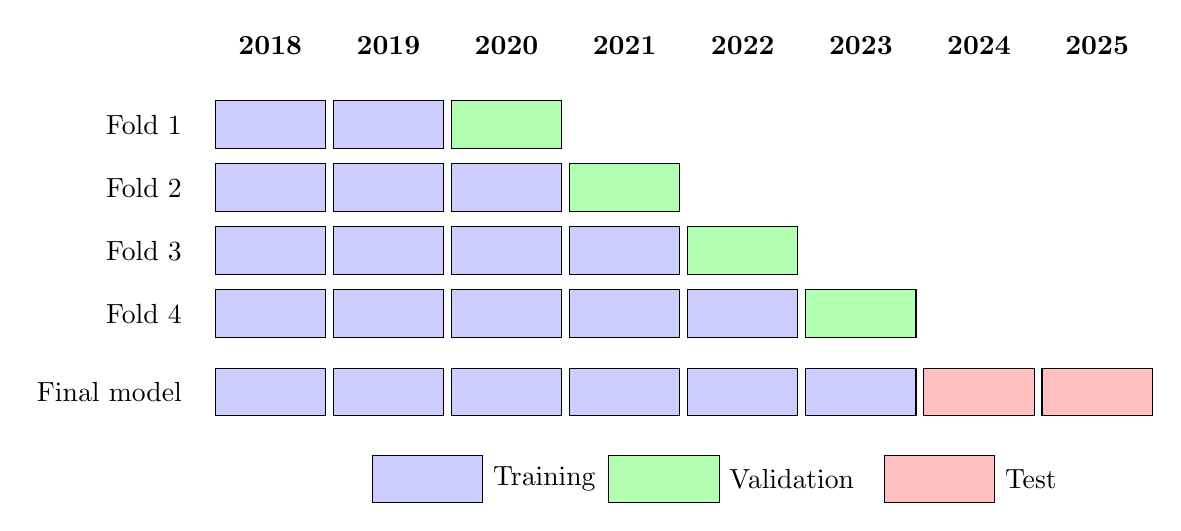
\begin{tikzpicture}[
    year/.style={draw, minimum width=1.4cm, minimum height=0.6cm},
    train/.style={year, fill=blue!20},
    valid/.style={year, fill=green!30},
    test/.style={year, fill=red!25}
]

% Year labels
\node at (0,3.5) {};
\foreach \x/\y in {0/2018,1.5/2019,3/2020,4.5/2021,6/2022,7.5/2023,9/2024,10.5/2025}
{
    \node at (\x,4) {\textbf{\y}};
}

% Fold 1
\node[left] at (-1,3) {Fold 1};
\node[train] at (0,3) {};
\node[train] at (1.5,3) {};
\node[valid] at (3,3) {};

% Fold 2
\node[left] at (-1,2.2) {Fold 2};
\node[train] at (0,2.2) {};
\node[train] at (1.5,2.2) {};
\node[train] at (3,2.2) {};
\node[valid] at (4.5,2.2) {};

% Fold 3
\node[left] at (-1,1.4) {Fold 3};
\node[train] at (0,1.4) {};
\node[train] at (1.5,1.4) {};
\node[train] at (3,1.4) {};
\node[train] at (4.5,1.4) {};
\node[valid] at (6,1.4) {};

% Fold 4
\node[left] at (-1,0.6) {Fold 4};
\node[train] at (0,0.6) {};
\node[train] at (1.5,0.6) {};
\node[train] at (3,0.6) {};
\node[train] at (4.5,0.6) {};
\node[train] at (6,0.6) {};
\node[valid] at (7.5,0.6) {};

% Final test
\node[left] at (-1,-0.4) {Final model};
\node[train] at (0,-0.4) {};
\node[train] at (1.5,-0.4) {};
\node[train] at (3,-0.4) {};
\node[train] at (4.5,-0.4) {};
\node[train] at (6,-0.4) {};
\node[train] at (7.5,-0.4) {};
\node[test] at (9,-0.4) {};
\node[test] at (10.5,-0.4) {};

% Legend
\node[train, label=right:Training] at (2,-1.5) {};
\node[valid, label=right:Validation] at (5,-1.5) {};
\node[test, label=right:Test] at (8.5,-1.5) {};

\end{tikzpicture}
\caption{Expanding-window temporal cross-validation used for model development. The final model is retrained on the complete development period (2018--2023) before evaluation on the independent test period (2024--2025).}
\label{fig:temporal_cv}
\end{figure}


Temporal cross-validation is chosen because drought impacts are expected to depend on conditions in previous years. For example, systems may be more or less vulnerable depending on antecedent soil moisture conditions or whether they have already been affected by previous drought impacts. Using an expanding temporal split therefore better reflects the real-world forecasting setting and avoids information leakage from future observations.


The period from 2024 to 2025 is reserved as an independent test period. These years are not used during model optimization and are only used for the final evaluation of the selected model. This provides an estimate of the expected model performance when applied to unseen future drought events. The test period includes one relatively normal year (2024) and one drought year (2025), allowing the model to be evaluated under contrasting hydroclimatic conditions.
The automated optimization procedure searches over the predefined search space shown in Table~\ref{tab:search_space}. The search space consists of candidate machine learning algorithms, predictor and model-specific hyperparameter ranges. Each candidate configuration is evaluated using the expanding-window temporal cross-validation procedure described above, and the configuration with the highest validation performance is selected for the final model.

\begin{table}[h]
\centering
\caption{Search space explored during the automated model optimization procedure.}
\label{tab:search_space}
\begin{tabular}{p{4cm} p{10cm}}
\toprule
\textbf{Component} & \textbf{Search space} \\
\midrule
Machine learning models &
Logistic Regression, Elastic Net, Random Forest, XGBoost, CatBoost \\

Predictors  &
Candidate predictor configurations described in Table ~\ref{tab:predictor_space} \\

Hyperparameters &
Model-specific hyperparameter ranges \\

Validation strategy &
Expanding-window temporal cross-validation \\

Selection criterion &
Mean validation performance across all cross-validation folds \\
\bottomrule
\end{tabular}
\end{table}

After selecting the final model configuration, post-hoc analysis is performed using explainable artificial intelligence methods. These methods are used to analyse the contribution of individual predictor variables and improve the interpretation of the model predictions. This analysis provides insight into which drought characteristics, regional properties, and temporal variables contribute most strongly to drought impact occurrence.




\section{Results}

\section{Results}

\subsection{Selected model configuration}

The automated optimization procedure evaluated 100 candidate configurations, of
which 70 completed all four cross-validation folds and 30 were terminated early
by the median pruning rule. Model selection was based on the macro-averaged
area under the precision--recall curve (PR-AUC) at a one-month lead time,
averaged over the four expanding-window folds.

The selected configuration is a Random Forest classifier using 32 of the 52
candidate predictors, achieving a mean cross-validation macro PR-AUC of 0.324
(Table~\ref{tab:best_config}). Tree-based models dominated the upper range of
the search: across completed trials, Random Forest achieved a mean score of
0.305 and XGBoost 0.300, compared with 0.273 for CatBoost, 0.267 for Elastic
Net and 0.263 for Logistic Regression. Fold-level scores for the selected
configuration were 0.433 (validation year 2020), 0.193 (2021), 0.336 (2022) and
0.334 (2023). The comparatively poor performance in 2021 corresponds to a year
without a major drought event, indicating that predictive skill is concentrated
in drought years.

A notable outcome of the predictor search is that the standardized drought
indices (SPI and SPEI) were not retained. The optimization selected the
\textit{auxiliary} meteorological subset, consisting of soil moisture anomalies
and consecutive dry days, in preference to the SPI and SPEI accumulations.
All remaining predictor groups were retained, with the class-lag group
restricted to agricultural impact lags and the elevation group restricted to
mean elevation.

\begin{table}[h]
\centering
\small
\caption{Selected model configuration obtained from the automated optimization procedure.}
\label{tab:best_config}
\begin{tabular}{p{4.5cm} p{9.5cm}}
\toprule
\textbf{Component} & \textbf{Selected value} \\
\midrule
Algorithm & Random Forest \\
Hyperparameters & 400 trees, maximum depth 6, minimum samples per leaf 9, balanced subsample class weighting \\
Number of predictors & 32 (of 52 candidates) \\
Hydro-meteorological & Soil moisture anomaly, consecutive dry days \\
Regional characteristics & Land cover (3), population fraction, mean elevation, soil composition (18) \\
Temporal & Seasonal harmonics, previous impact occurrence, agricultural impact lags (4) \\
Cross-validation macro PR-AUC ($h=1$) & 0.324 \\
\bottomrule
\end{tabular}
\end{table}

\subsection{Forecast performance on the independent test period}

The selected configuration was retrained on the complete development period
(2018--2023) and evaluated on the independent test period (2024--2025), which
comprises 837 region--month observations across 40 NUTS-3 regions.
Table~\ref{tab:test_horizon} reports macro-averaged performance for each
forecast horizon.

Because the impact classes are rare, PR-AUC values must be interpreted relative
to the class prevalence, which represents the expected performance of a
no-skill classifier. The skill score is therefore defined as the difference
between the observed PR-AUC and the prevalence.

At a one-month lead time the model achieves a macro PR-AUC of 0.324 against a
macro prevalence of 0.091, corresponding to a skill of 0.233 and a 3.6-fold
improvement over the no-skill baseline. Performance decreases monotonically
with lead time, from a skill of 0.247 at $h=0$ to 0.182 at $h=3$, while
remaining approximately 2.9 times better than the baseline at the longest
horizon. This gradual decline is consistent with the expectation that
predictive skill decreases with increasing lead time, but indicates that useful
skill is retained across the full zero-to-three-month range rather than
collapsing to random performance.

\begin{table}[h]
\centering
\small
\caption{Macro-averaged test performance by forecast horizon (2024--2025, ten impact classes).}
\label{tab:test_horizon}
\begin{tabular}{lrrrrrrr}
\toprule
\textbf{Horizon} & \textbf{PR-AUC} & \textbf{Prevalence} & \textbf{Skill} & \textbf{ROC-AUC} & \textbf{Precision} & \textbf{Recall} & \textbf{Brier} \\
\midrule
$h=0$ & 0.340 & 0.093 & 0.247 & 0.779 & 0.240 & 0.606 & 0.150 \\
$h=1$ & 0.324 & 0.091 & 0.233 & 0.768 & 0.220 & 0.605 & 0.161 \\
$h=2$ & 0.285 & 0.094 & 0.191 & 0.744 & 0.190 & 0.608 & 0.177 \\
$h=3$ & 0.277 & 0.095 & 0.182 & 0.734 & 0.192 & 0.602 & 0.178 \\
\bottomrule
\end{tabular}
\end{table}

The model operates in a high-recall, low-precision regime, correctly
identifying approximately 60\% of impact occurrences at a precision of
0.19--0.24. This behaviour follows from the balanced class weighting applied
during training and is appropriate for an early-warning context, in which
failing to anticipate an impact is generally more costly than issuing a false
alarm.

\subsection{Performance across impact classes}

Performance varies considerably between impact classes
(Table~\ref{tab:test_class}). Agricultural Economic Loss, Crop Failure and
Yield Reduction, Irrigation Shortage and Water Use Restrictions form a
consistently well-predicted group, with skill scores between 0.315 and 0.363
and ROC-AUC values approaching 0.83. These classes are directly coupled to the
agricultural water balance, which is well represented by the selected soil
moisture and dry-spell predictors.

A second group, comprising Reservoir and Surface Water Shortage, Forest Dieback
and Vegetation Stress, and Freshwater Ecosystem Degradation, is substantially
harder to predict, with skill scores of 0.103--0.143. These impacts depend on
accumulated hydrological deficits and ecological response times that are only
partially captured by the monthly predictors used here.

\begin{table}[h]
\centering
\small
\caption{Test performance by impact class at a one-month lead time ($h=1$), ordered by skill.}
\label{tab:test_class}
\begin{tabular}{p{6.2cm} rrrrr}
\toprule
\textbf{Impact class} & \textbf{Prev.} & \textbf{PR-AUC} & \textbf{Skill} & \textbf{ROC-AUC} & \textbf{Recall} \\
\midrule
Agricultural Economic Loss          & 0.035 & 0.398 & 0.363 & 0.832 & 0.621 \\
Crop Failure \& Yield Reduction     & 0.148 & 0.478 & 0.330 & 0.797 & 0.629 \\
Irrigation Shortage                 & 0.088 & 0.412 & 0.323 & 0.822 & 0.635 \\
Water Use Restrictions              & 0.059 & 0.374 & 0.315 & 0.794 & 0.694 \\
Groundwater Depletion               & 0.109 & 0.377 & 0.268 & 0.752 & 0.637 \\
Wildfire Occurrence                 & 0.029 & 0.220 & 0.191 & 0.799 & 0.625 \\
Water Supply \& Sanitation Issues   & 0.111 & 0.269 & 0.157 & 0.750 & 0.570 \\
Freshwater Ecosystem Degradation    & 0.117 & 0.260 & 0.143 & 0.678 & 0.551 \\
Forest Dieback \& Vegetation Stress & 0.111 & 0.250 & 0.139 & 0.734 & 0.613 \\
Reservoir \& Surface Water Shortage & 0.103 & 0.206 & 0.103 & 0.718 & 0.477 \\
\bottomrule
\end{tabular}
\end{table}

\subsection{Temporal variation in forecast skill}

Forecast skill is strongly seasonal (Figure~\ref{fig:diag_calendar_month}).
Skill is highest during the summer months, reaching 0.490 in August, 0.414 in
July and 0.359 in June, and remains substantial in March (0.371) and April
(0.300). In January, October and November the number of observed impacts is too
small for PR-AUC to be defined, and these months are therefore reported as
missing rather than as zero skill. This reflects the seasonal concentration of
drought impacts in the database rather than a failure of the model.

Skill also depends on the prevailing drought regime
(Table~\ref{tab:drought_bin}). Under dry conditions, defined by an SPEI-12
value below $-1$, the model achieves a macro PR-AUC of 0.440 and a skill of
0.296. Under near-normal conditions skill decreases to 0.224, and under wet
conditions to 0.133. The model therefore performs best precisely in the
conditions under which impact-based drought forecasting is operationally
relevant.

\begin{table}[h]
\centering
\small
\caption{Test performance by SPEI-12 drought regime at $h=1$.}
\label{tab:drought_bin}
\begin{tabular}{lrrrrr}
\toprule
\textbf{Drought regime} & \textbf{Observations} & \textbf{Positives} & \textbf{Prevalence} & \textbf{PR-AUC} & \textbf{Skill} \\
\midrule
Dry         & 1410 & 187 & 0.133 & 0.440 & 0.296 \\
Near-normal & 1650 & 290 & 0.176 & 0.400 & 0.224 \\
Wet         & 5310 & 284 & 0.053 & 0.187 & 0.133 \\
\bottomrule
\end{tabular}
\end{table}

\subsection{Spatial variation in forecast skill}

Regional performance was evaluated for each NUTS-3 region separately
(Figure~\ref{fig:diag_choropleth}). Of the 40 regions, 15 contain sufficient
positive observations in the test period for regional skill to be computed;
for the remaining regions the metric is undefined and these are shown as
missing. This sparsity is a direct consequence of the chosen spatial
resolution: disaggregating a limited number of reported impacts across 40
regions and 21 test months leaves many region--class combinations empty.

Among the regions where skill can be estimated, Groot-Rijnmond attains the
highest value (0.507), followed by Zuidoost-Noord-Brabant (0.397),
Zeeuwsch-Vlaanderen (0.369) and Zuid-Limburg (0.340). The lowest values occur
in Veluwe (0.114), Delft en Westland (0.115) and Utrecht (0.146). The
better-performing regions are predominantly located in the southern and
south-western Netherlands, which correspond to the areas most frequently
affected during the 2018, 2019 and 2022 drought events and therefore provide
the richest training signal.

\subsection{Predictor contributions}

Post-hoc interpretation was performed using SHAP values computed on the test
period at a one-month lead time, averaged across the ten class-specific models
(Figure~\ref{fig:shap}). The dominant predictor is the seasonal cosine
component (mean $|$SHAP$|$ = 0.070), confirming that the annual cycle of
drought impacts is the single strongest signal available to the model. This is
followed by consecutive dry days (0.047), the peat soil fraction (0.034) and
the soil moisture anomaly (0.031).

Two observations follow from this ranking. First, the two retained
hydro-meteorological predictors rank second and fourth overall, confirming
that the optimization procedure discarded the SPI and SPEI accumulations
because they were redundant rather than uninformative. Second, static soil
composition variables occupy several of the leading positions, with peat and
peaty soils contributing most strongly. This supports the inclusion of soil
composition proposed during the exploratory analysis and expert consultation,
and is physically consistent with the elevated drought sensitivity of
organic-rich soils in the Netherlands.

\subsection{Predictability limits across impact classes}

To assess whether the restriction to the ten most frequent impact classes is
justified, a supplementary analysis scored all fifteen candidate classes under
a single shared model configuration using the same cross-validation procedure
(Table~\ref{tab:predictability}). A class was considered predictable if it
achieved a cross-validation skill of at least 0.15 and a PR-AUC of at least
0.25.

Seven classes satisfy both criteria, with skill scores between 0.170 and 0.263.
The remaining eight fall below the threshold, and the lowest-ranked classes
(Inland Waterway Disruption, Broader Economic Disruption, Social Impacts and
Wetland Loss) achieve skill scores below 0.05, indicating essentially no
predictive signal. These classes are both rare and only indirectly related to
hydro-meteorological conditions, and their occurrence in the database is
strongly influenced by media reporting behaviour rather than physical drought
severity.

This result confirms that predictive capability is limited to a subset of
impact types and supports the decision to restrict the prediction target to the
most frequently occurring classes. A second optimization stage restricted to
the predictable classes was also evaluated but did not improve performance
relative to the shared configuration (macro PR-AUC 0.374 versus 0.385), and the
single shared configuration was therefore retained.

\begin{table}[h]
\centering
\small
\caption{Cross-validation predictability of all fifteen candidate impact classes at $h=1$ under a shared model configuration.}
\label{tab:predictability}
\begin{tabular}{p{6.2cm} rrrl}
\toprule
\textbf{Impact class} & \textbf{PR-AUC} & \textbf{Prev.} & \textbf{Skill} & \textbf{Predictable} \\
\midrule
Forest Dieback \& Vegetation Stress & 0.396 & 0.133 & 0.263 & Yes \\
Groundwater Depletion               & 0.459 & 0.212 & 0.247 & Yes \\
Irrigation Shortage                 & 0.333 & 0.101 & 0.232 & Yes \\
Reservoir \& Surface Water Shortage & 0.383 & 0.167 & 0.216 & Yes \\
Water Use Restrictions              & 0.322 & 0.120 & 0.202 & Yes \\
Freshwater Ecosystem Degradation    & 0.415 & 0.215 & 0.200 & Yes \\
Crop Failure \& Yield Reduction     & 0.386 & 0.216 & 0.170 & Yes \\
\midrule
Wildfire Risk Increase              & 0.212 & 0.038 & 0.174 & No \\
Wildfire Occurrence                 & 0.185 & 0.043 & 0.143 & No \\
Agricultural Economic Loss          & 0.218 & 0.101 & 0.117 & No \\
Water Supply \& Sanitation Issues   & 0.243 & 0.157 & 0.086 & No \\
Wetland Loss                        & 0.095 & 0.052 & 0.043 & No \\
Social Impacts                      & 0.094 & 0.053 & 0.042 & No \\
Broader Economic Disruption         & 0.121 & 0.087 & 0.035 & No \\
Inland Waterway Disruption          & 0.064 & 0.038 & 0.026 & No \\
\bottomrule
\end{tabular}
\end{table}




%here methods
%resutls 
%disscusion
%limitations
\label{ch:baseline_model}







% -----
% -----






% \section{Data Synthesis: Meteorological and Impact Data}

% ideaziation, 

% we peform , ibf, but then
% we let the user show most likely 
% repeated news's artilce's.

% So basilay we show the set of news-artilce's,

% the prediction was based on the.

% The user can go back to source artilcle,  
% then be like oh, 
% these article's,  might repeat itself or might not
% repeat itself.



% \section{Baseline Predictive Models}
%     \subsection{Linear Models}
%     \subsection{Tree-Based Models}
%     \subsection{Meteorological-Only Benchmark}

% \section{Baseline Performance Evaluation}




\chapter{Research outputs}

\section{Drought impact Database}
% For the drought impact base the research outputs, mainly consist of an spatial temparal nalysis of the data.
% The goal of this chapter is to provide an birds eye vieuw of all the data we have collected. What biases are in our data and what pattern's do frequenly occur in our data? Are there any temporal biases, are there any spatial biases. If we would build an model in the future, where should we start, what can we infer based of our simple plots. 



% Firstly in this section we provide an bird-eye vieuw of the netlherands. We plot some general stats about our database. Spatial, and temporal.  insert plots >spatial aggreated counts, what regions have the most impacts<, 
% and temporal how do impcats counts in genral evolve over time.


% Then we coonclude like that we have to do an data split based of time, and we sort of identify , two reporting regions pre-2018, and after 2018. Based on these splits, we will try to check how they correlate compared to the kmidrought composlite index, with an nrmolized impact ocunts plot for both feature's here we mianly ask, do the impact counts overlapp with drought periods? 




% In chpater valiation, we validated the data accros other proxy datasets. 

% The goal of this section, is different. It sort of has to provide an births-eye view of all the data we collected. The main question this should anwser to our stakeholder's is: what could we potentially do with this dataset? Do we have enough impacts to build an machine learning model? What drought impacts occur where and how often and at the right timing? 


% First of we start by analysing the general drought impact trend from our news-archive's. 

% >Insert plot<
% Heat-map per category + average impacts per year +

% years, drought index, category normalized.
% ------------------------------







% to find out how many impact we have and if they are good enough for machine learning, we require our impacts to be spatially and temporal be distrubted in an logical and sound way. 

% 1. total impact counts per category
% 2. mean variance per year














% Observe that there is an relationship between how much reporting there is done in general in the Netherlands and the amount of impact counts. The discrepancy between reported impacts in 2005 and 2020, could also be explained by different reporting practise's (the observered world) and not an actual changes in the real world.


% We therefor, present the data in 



% So we also want to visualize general trends in the impact database, but to do so we require





% then 



% First of how much data do we have in general, how much data do we have for a certain category. This gives us insights, in the spatial properties of the 

% Do general trends, in the data set compared to drought events make sense.

% Decide what visulizations we need:


% 0. General news-artilce counts 

% ---> motivate our impact aggregatoin method


% 1. amount of impacts for an specicif sub-category over year.

% Do normalized theme, and at an drougt index? maybe min max normalize for +/- 2.5 years,

% idea is to have an local and global variable. 



% 2. Percentage impact sub-plot.

% What regions have highest impact occurence's. so bassilcy we +/- for an specif impact an NL plot.

% these should be 20 plots. ---> use nuts3 aggregation framework to excute this.

% ---------------------------------------------------
% tldr.





\section{Impact based forecasting}



% ==========================================
% \chapter{Multi-Source Feature Integration and Analysis}
% \label{ch:feature_integration}
% % ==========================================

% \section{Hydrological Feature Integration}
%     \subsection{Groundwater Dynamics}
%     \subsection{River Discharge Variables}

% \section{Socio-Economic Exposure Indicators}

% \section{Feature Contribution and Importance Analysis}

% \section{Ablation Study on Data Source Contribution}


% % ==========================================
% \chapter{Results and Discussion}
% \label{ch:results}
% % ==========================================

% \section{Predictive Performance Comparison}

% \section{Spatial Patterns of Drought Impact Risk in the Netherlands}

% \section{Implications for Dutch Water Management}

% \section{Limitations and Sources of Uncertainty}


% ==========================================
\chapter{Conclusion}
% ==========================================

\section{Synthesis of Research Contributions}



\section{Implications for Impact-Based Forecasting}

\section{Recommendations for Dutch Water Management}

\section{Future Research Directions}

% --- Back Matter ---
\appendix
\chapter{Technical Specifications}
\chapter{Supplementary Results and Data Tables}
contact personen Femke strasvoort
margreet van landne (zie droogte 2022)

\chapter{Drought Impact Database}
\begin{figure}[!ht]
    \centering
    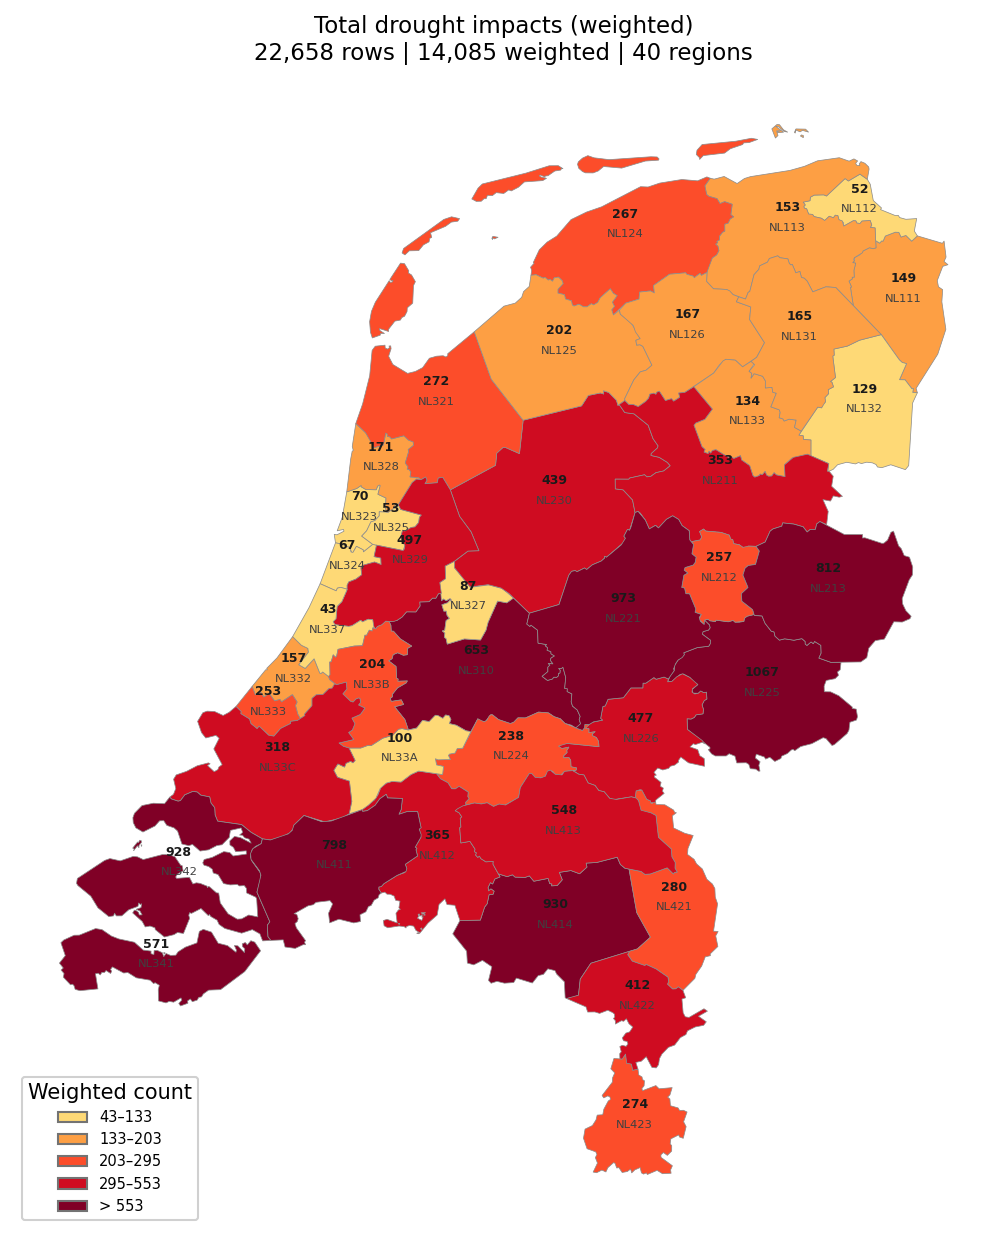
\includegraphics[width=0.65\textwidth]{figures/Appendix C images/choropleth_total_impacts.png}
    \caption{Spatial distribution of the total number of drought impacts extracted from newspaper articles between 2000 and 2025.}
    \label{fig:choropleth_total_impacts}
\end{figure}

\begin{figure}[p]
\centering

% Row 1
\begin{subfigure}{0.30\textwidth}
    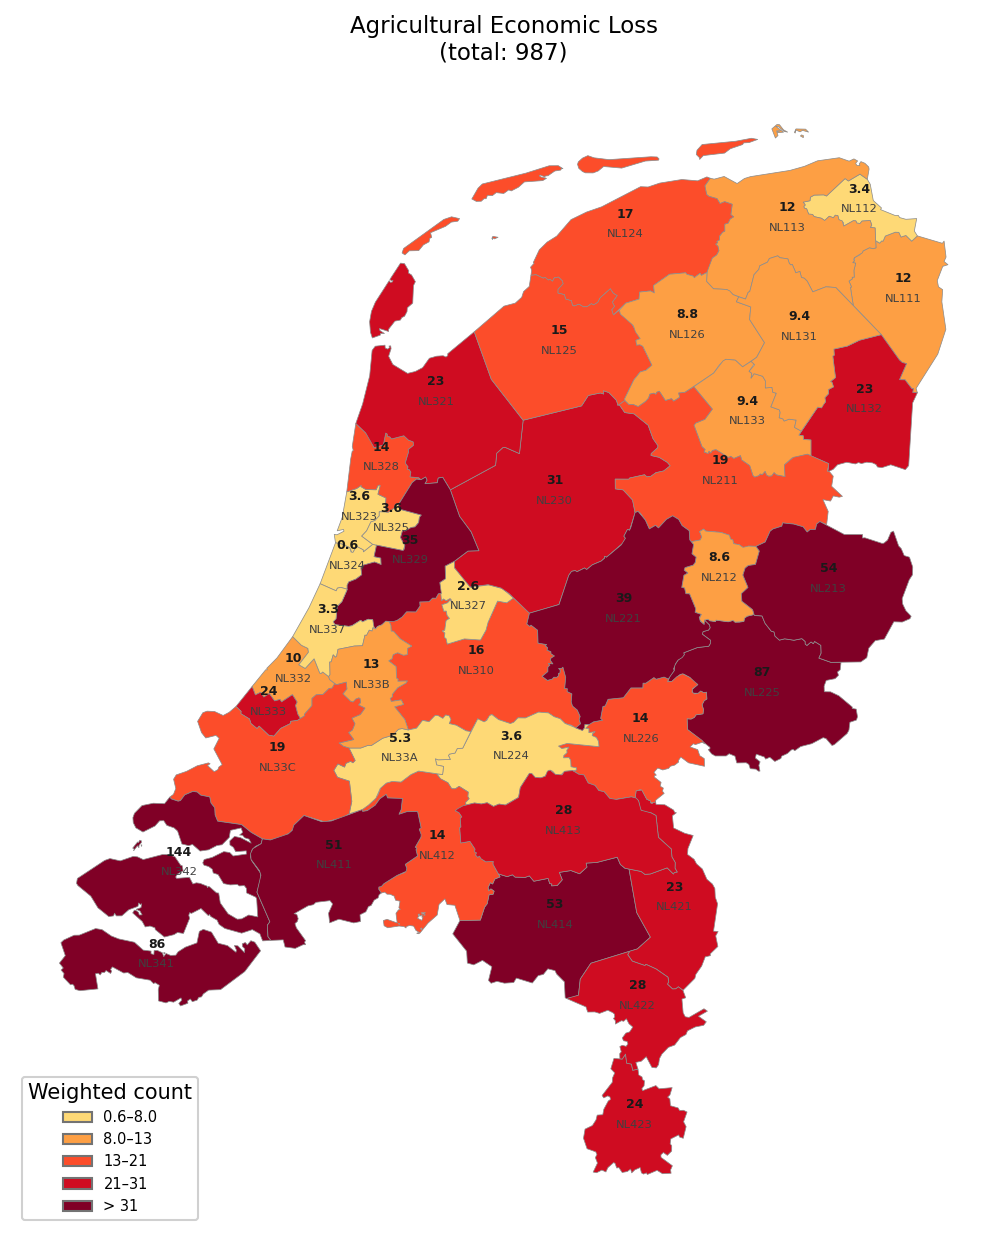
\includegraphics[width=\linewidth]{figures/Appendix C images/choropleth_agricultural_economic_loss.png}
    \caption{Agricultural economic loss}
\end{subfigure}
\hfill
\begin{subfigure}{0.30\textwidth}
    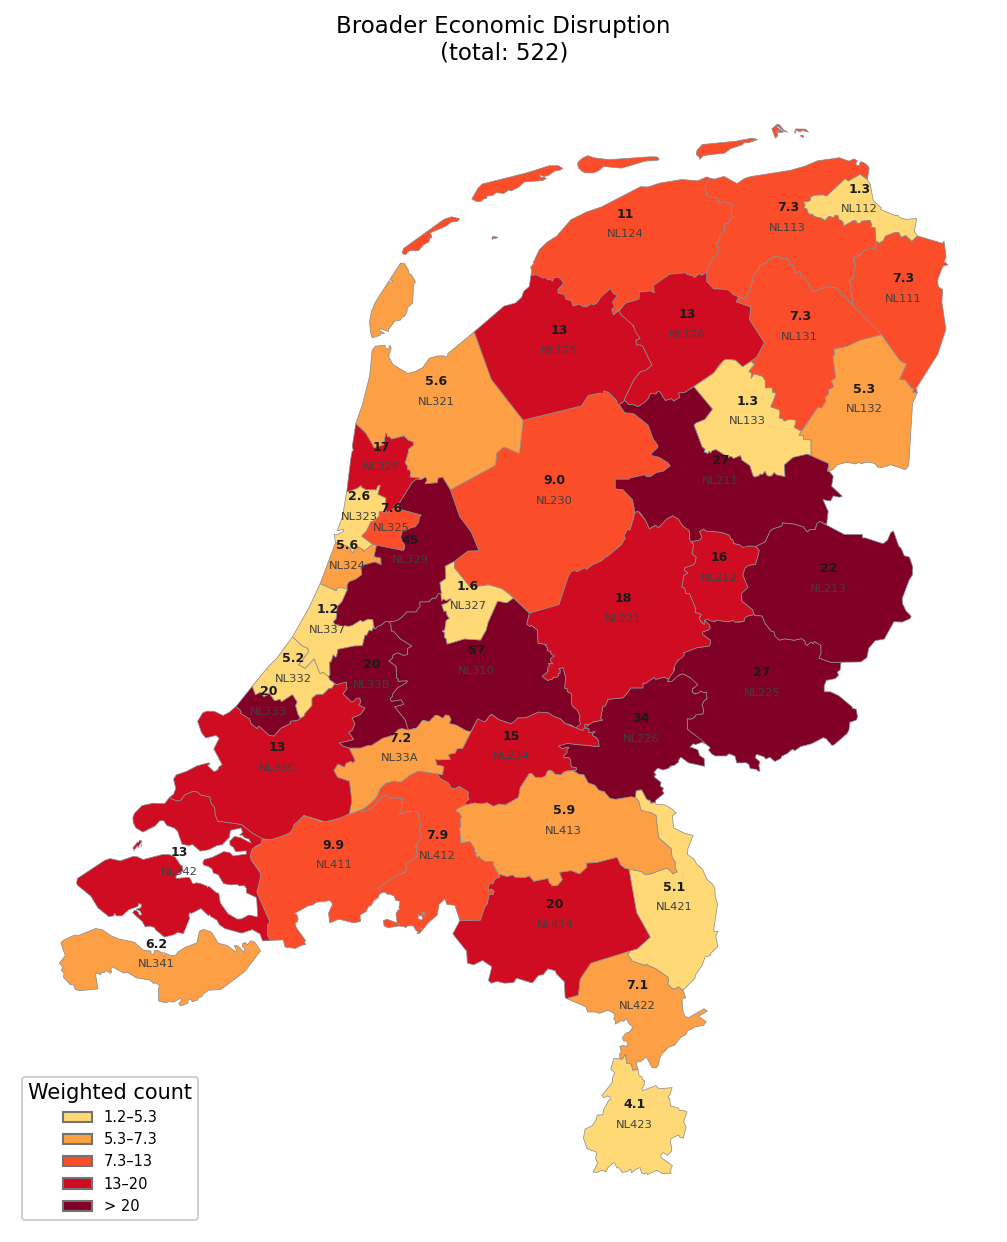
\includegraphics[width=\linewidth]{figures/Appendix C images/choropleth_broader_economic_disruption.png}
    \caption{Broader economic disruption}
\end{subfigure}
\hfill
\begin{subfigure}{0.30\textwidth}
    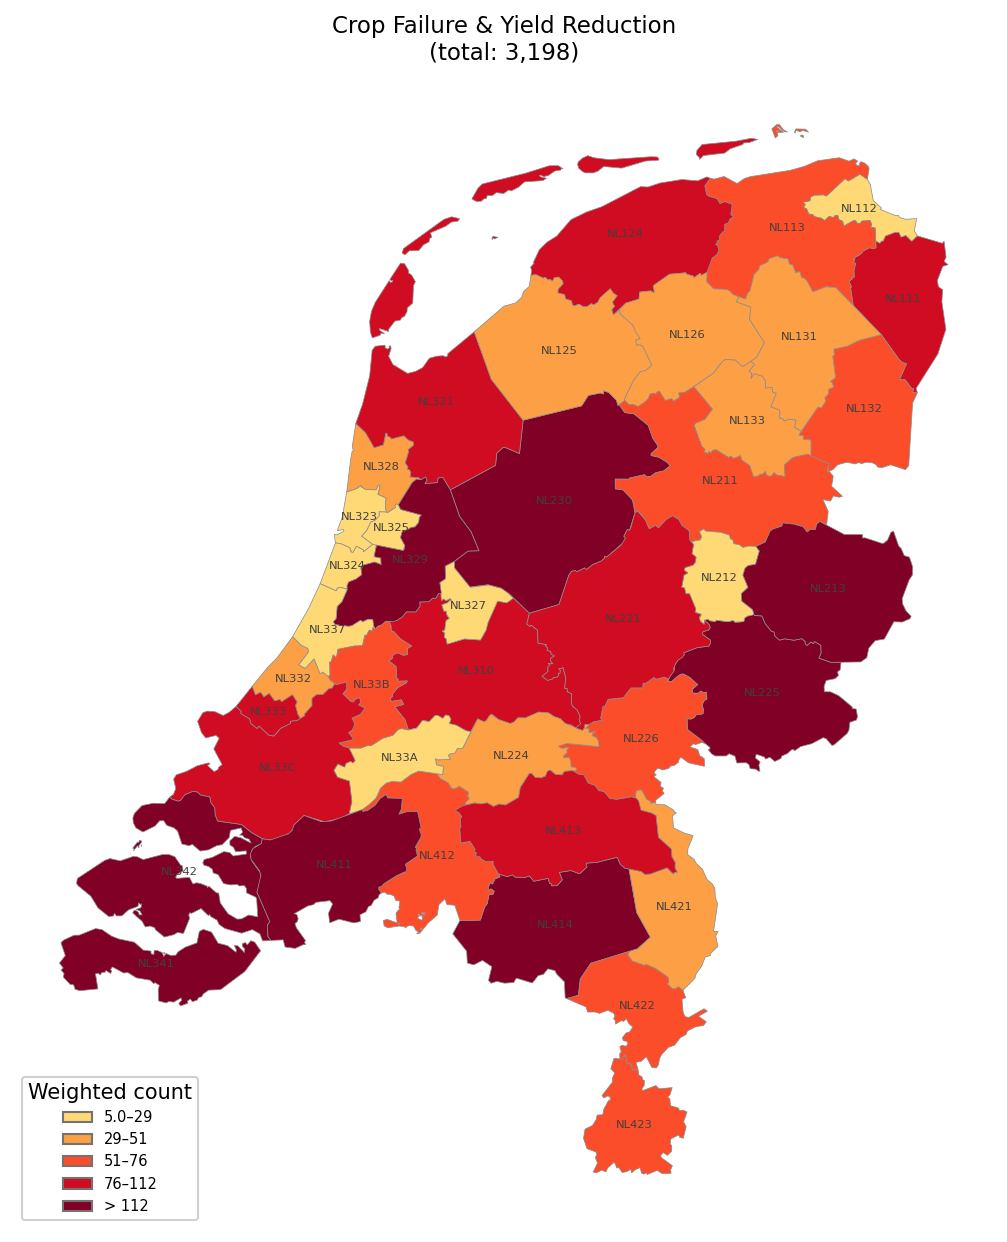
\includegraphics[width=\linewidth]{figures/Appendix C images/choropleth_crop_failure_yield_reduction.png}
    \caption{Crop failure and yield reduction}
\end{subfigure}

\vspace{0.5cm}

% Row 2
\begin{subfigure}{0.30\textwidth}
    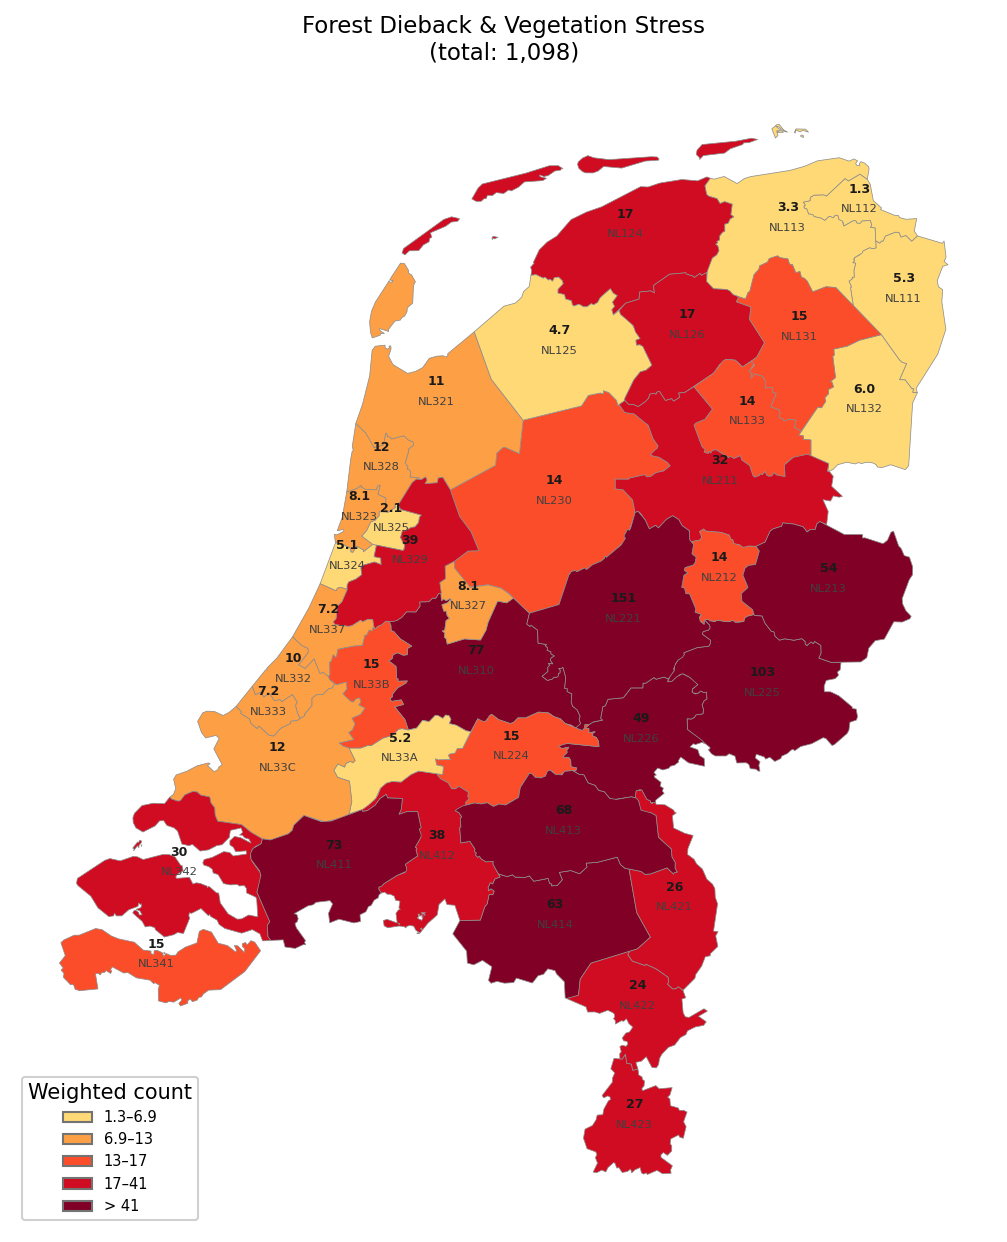
\includegraphics[width=\linewidth]{figures/Appendix C images/choropleth_forest_dieback_vegetation_stress.png}
    \caption{Forest dieback and vegetation stress}
\end{subfigure}
\hfill
\begin{subfigure}{0.30\textwidth}
    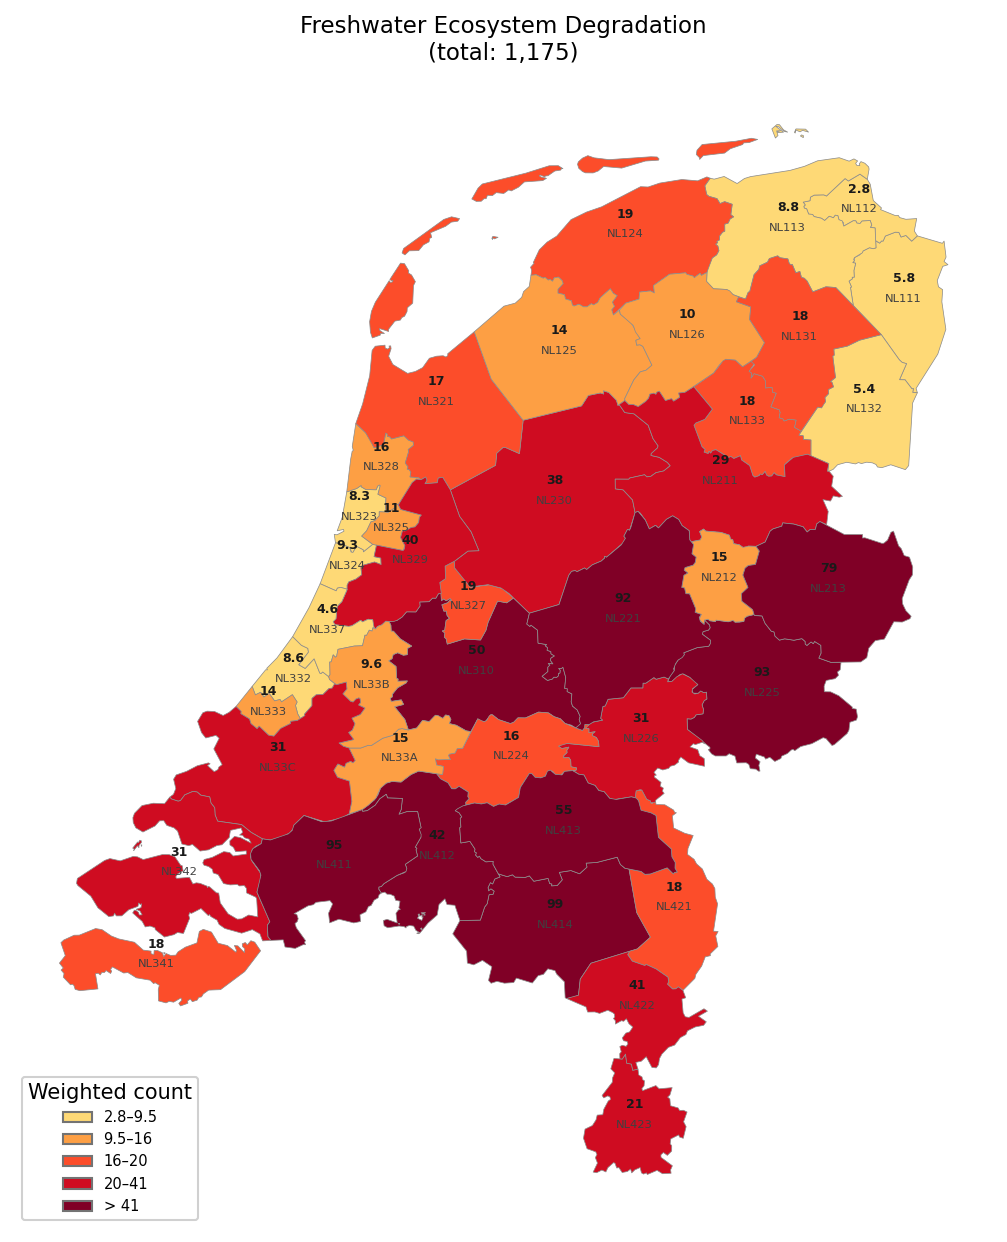
\includegraphics[width=\linewidth]{figures/Appendix C images/choropleth_freshwater_ecosystem_degradation.png}
    \caption{Freshwater ecosystem degradation}
\end{subfigure}
\hfill
\begin{subfigure}{0.30\textwidth}
    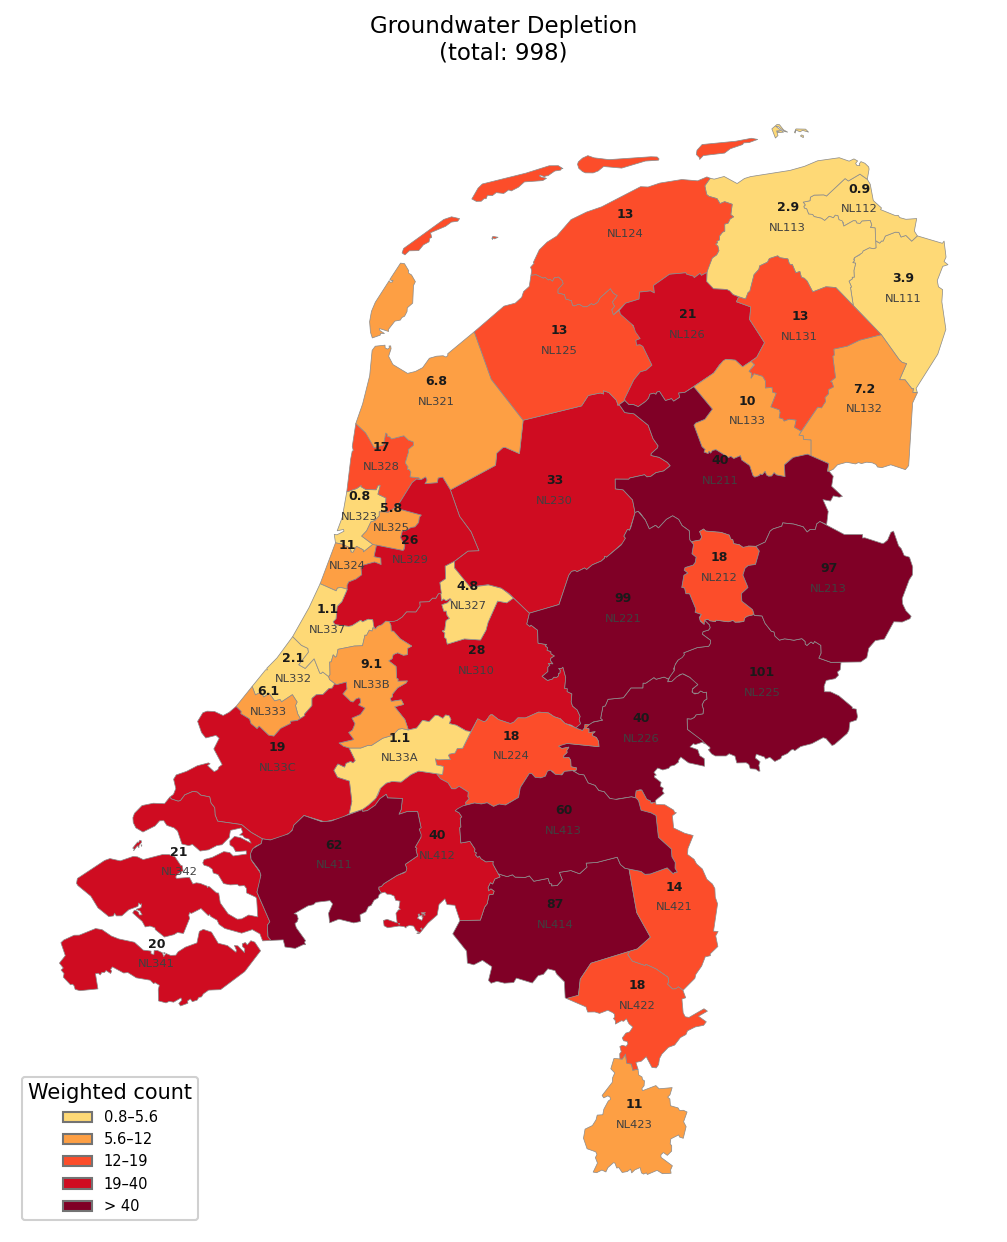
\includegraphics[width=\linewidth]{figures/Appendix C images/choropleth_groundwater_depletion.png}
    \caption{Groundwater depletion}
\end{subfigure}

\vspace{0.5cm}

% Row 3
\begin{subfigure}{0.30\textwidth}
    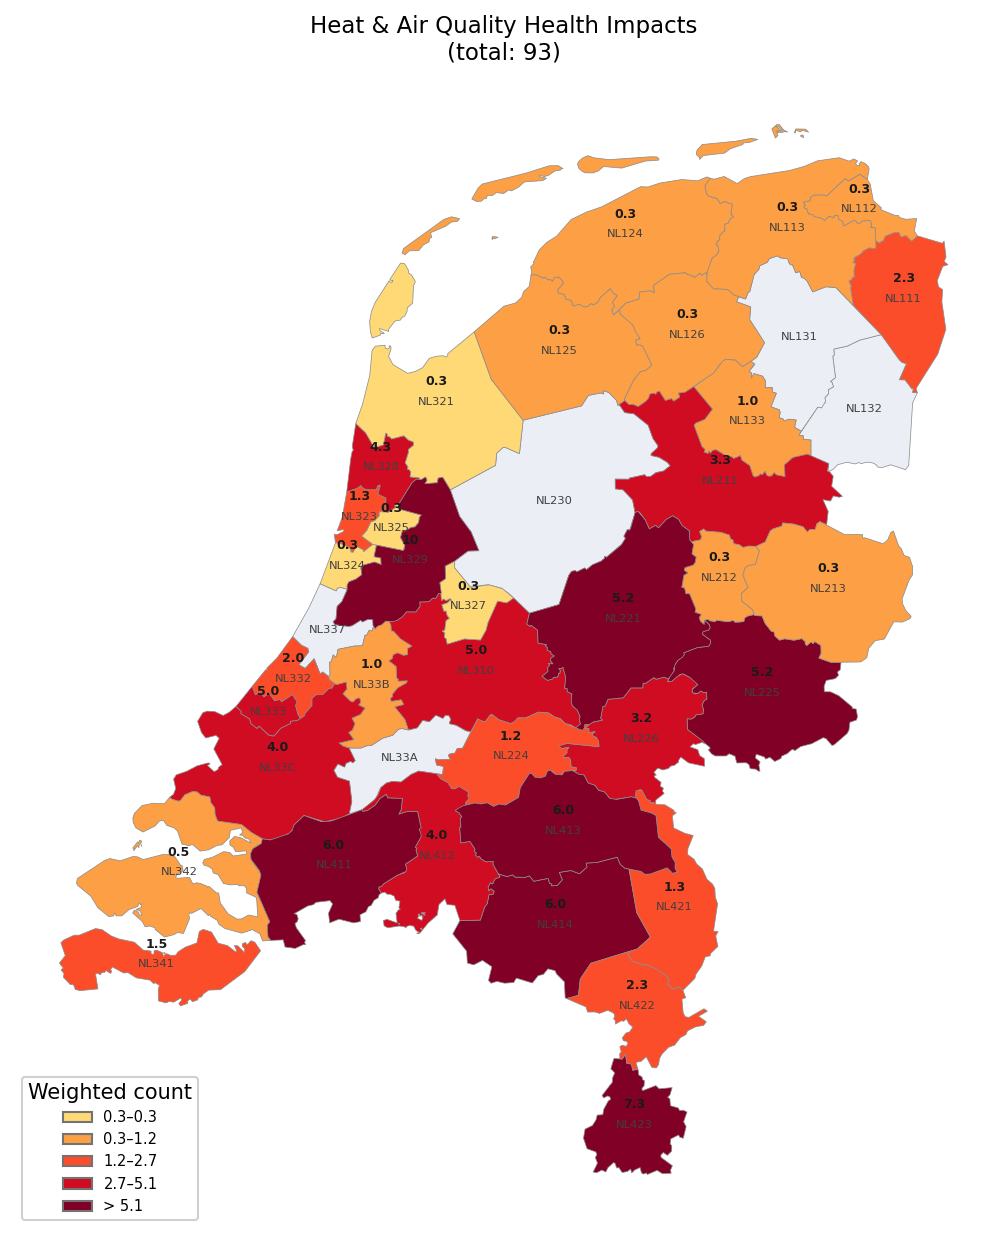
\includegraphics[width=\linewidth]{figures/Appendix C images/choropleth_heat_air_quality_health_impacts.png}
    \caption{Heat, air quality and health impacts}
\end{subfigure}
\hfill
\begin{subfigure}{0.30\textwidth}
    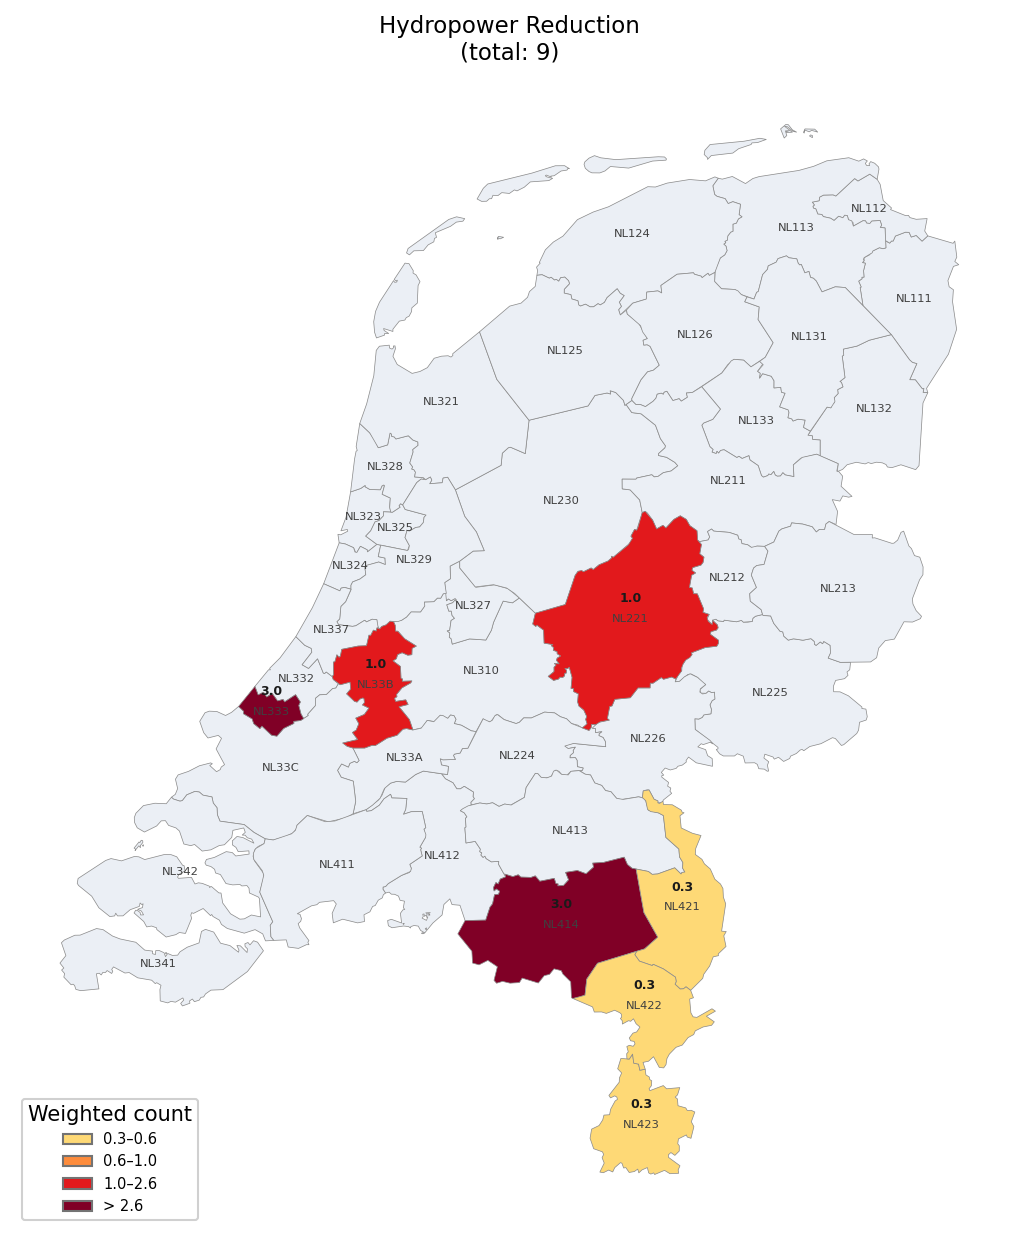
\includegraphics[width=\linewidth]{figures/Appendix C images/choropleth_hydropower_reduction.png}
    \caption{Hydropower reduction}
\end{subfigure}
\hfill
\begin{subfigure}{0.30\textwidth}
    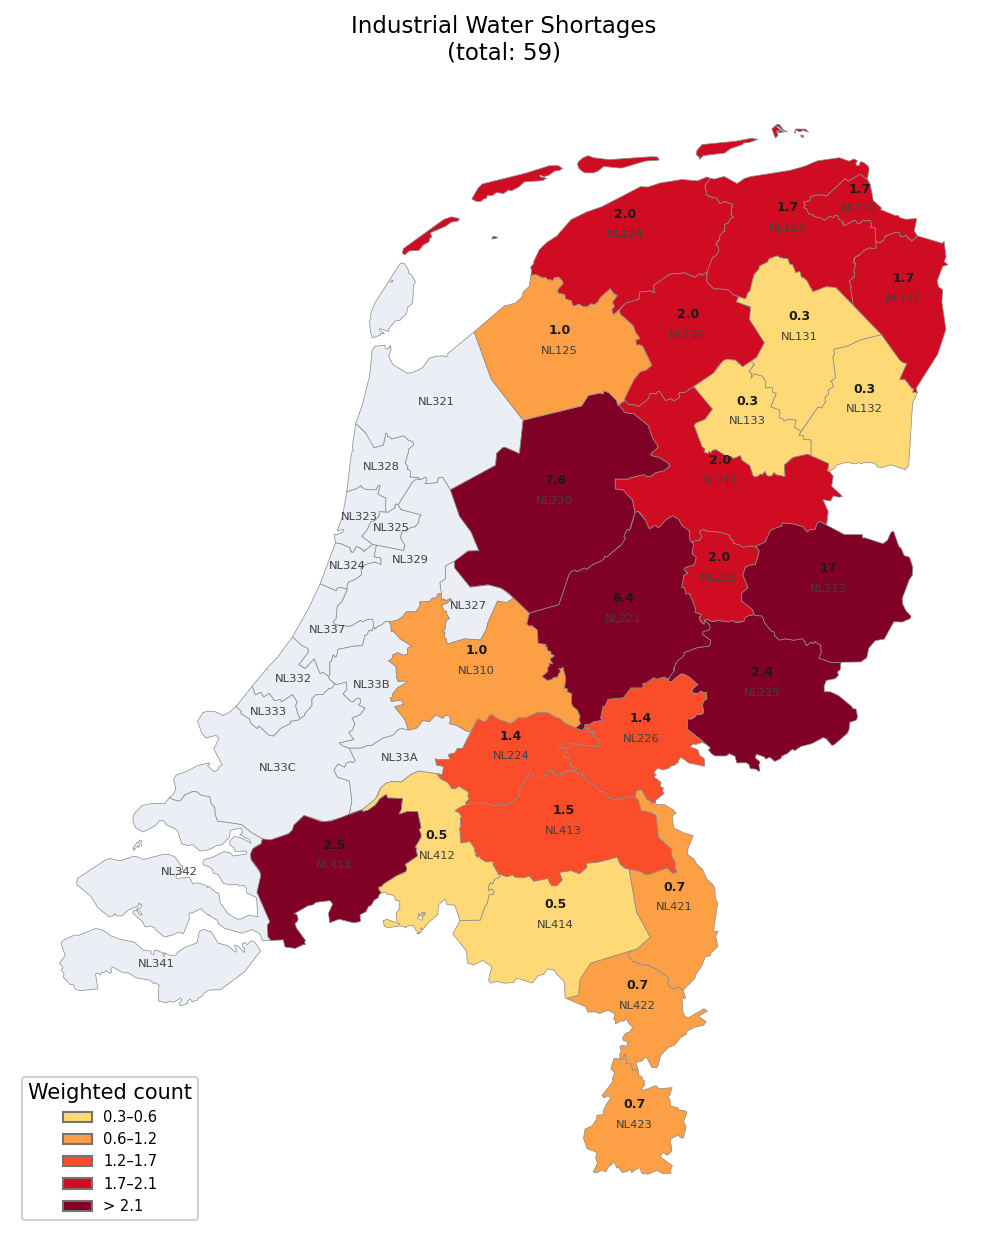
\includegraphics[width=\linewidth]{figures/Appendix C images/choropleth_industrial_water_shortages.png}
    \caption{Industrial water shortages}
\end{subfigure}

\caption{Spatial distribution of drought impacts (Part 1).}
\label{fig:appendix_choropleths_1}
\end{figure}



\begin{figure}[p]
\centering

% Row 1
\begin{subfigure}{0.32\textwidth}
    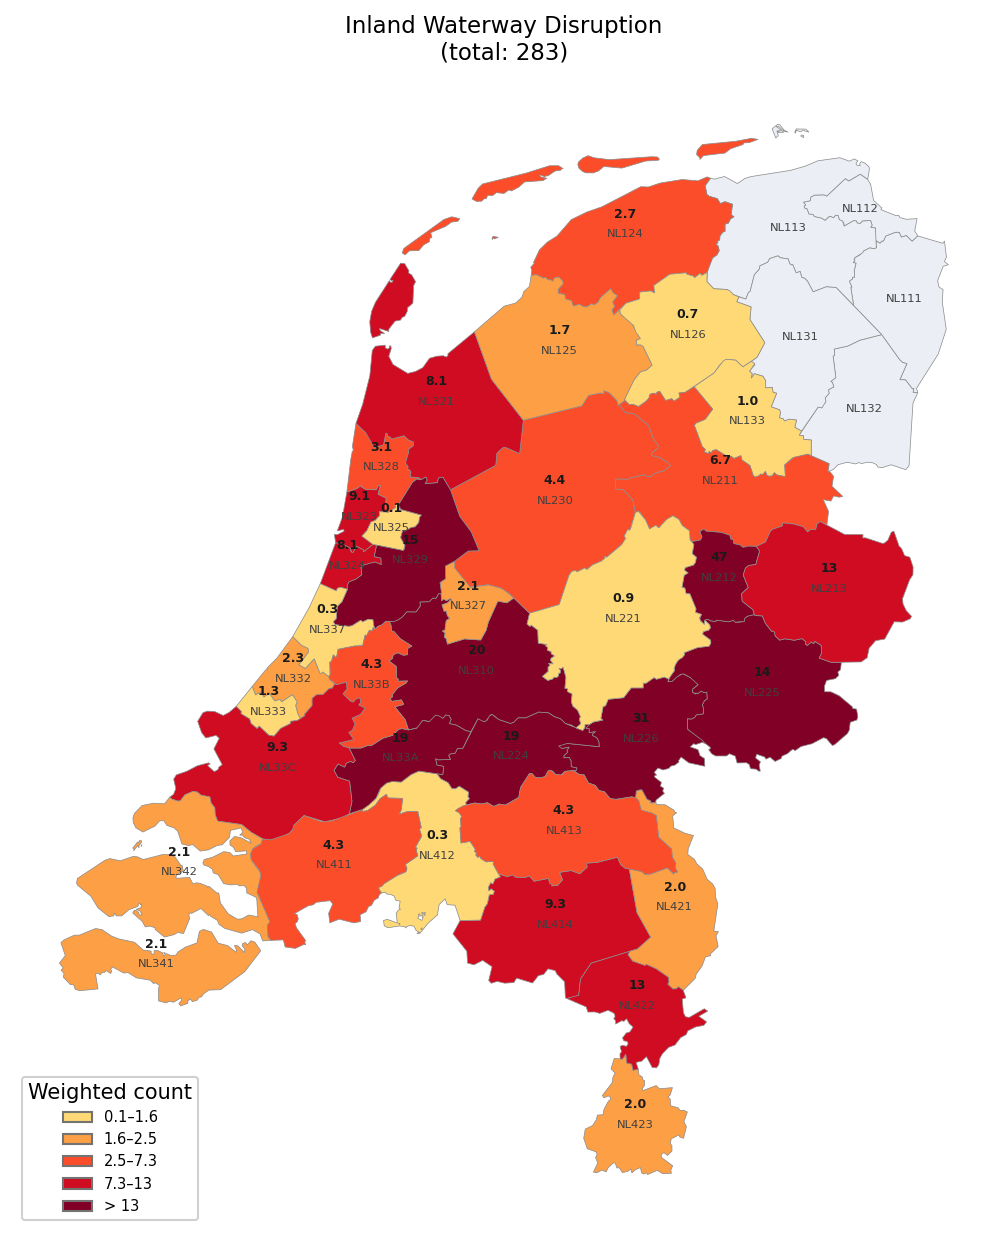
\includegraphics[width=\linewidth]{figures/Appendix C images/choropleth_inland_waterway_disruption.png}
    \caption{Inland waterway disruption}
\end{subfigure}
\hfill
\begin{subfigure}{0.32\textwidth}
    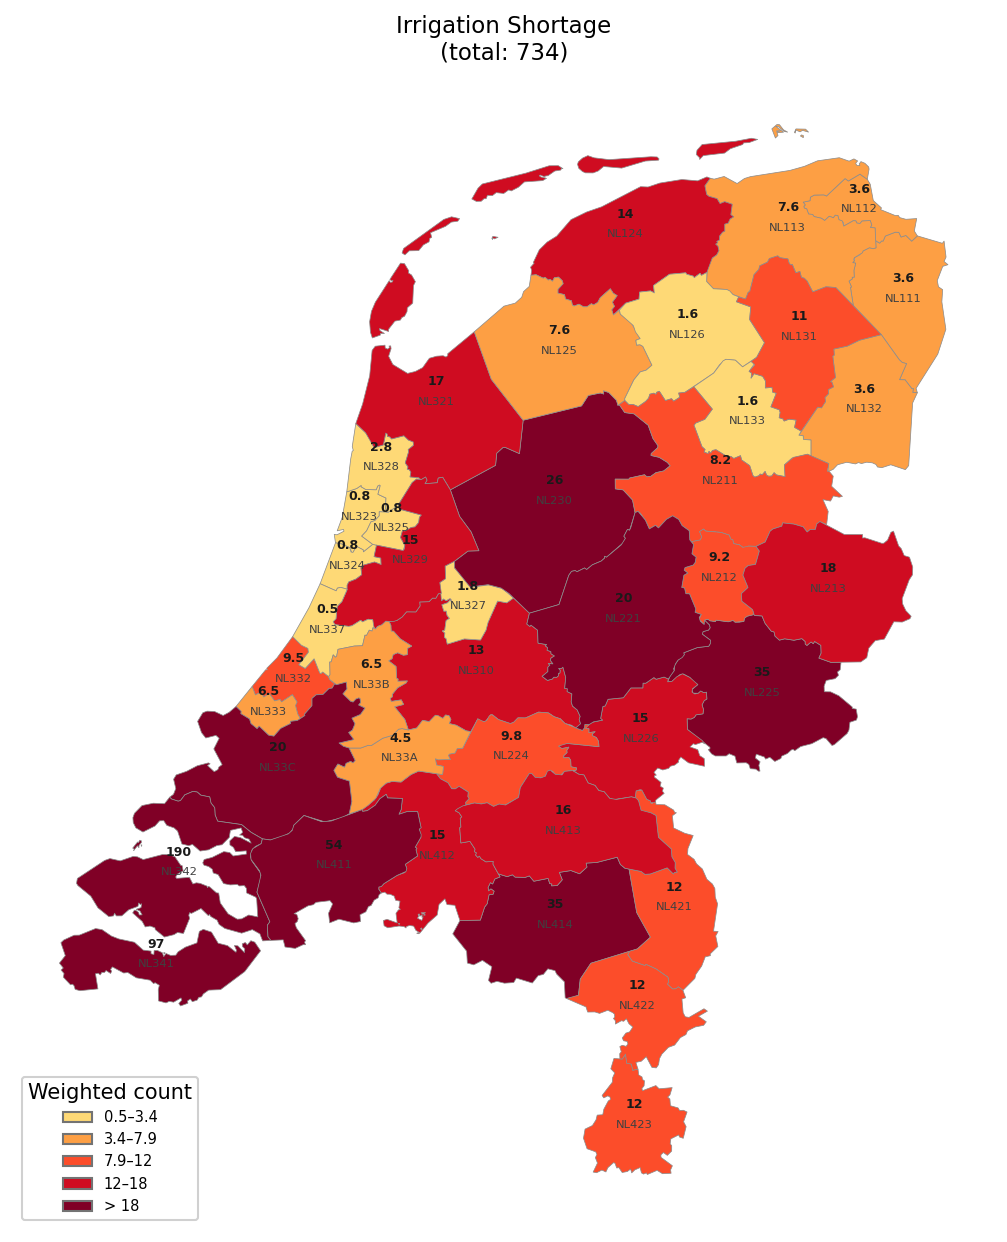
\includegraphics[width=\linewidth]{figures/Appendix C images/choropleth_irrigation_shortage.png}
    \caption{Irrigation shortage}
\end{subfigure}
\hfill
\begin{subfigure}{0.32\textwidth}
    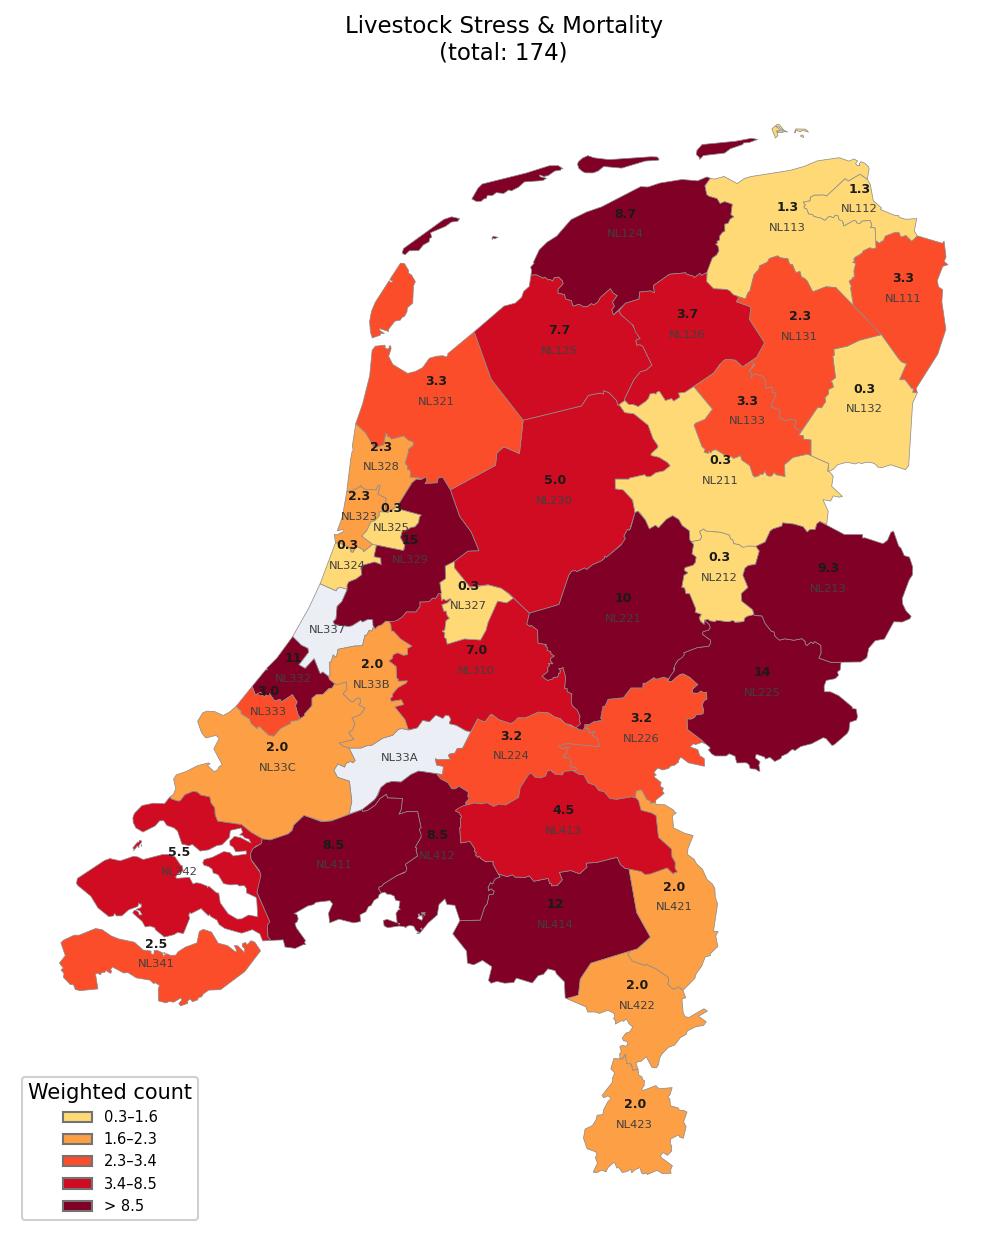
\includegraphics[width=\linewidth]{figures/Appendix C images/choropleth_livestock_stress_mortality.png}
    \caption{Livestock stress and mortality}
\end{subfigure}

\vspace{0.5cm}

% Row 2
\begin{subfigure}{0.32\textwidth}
    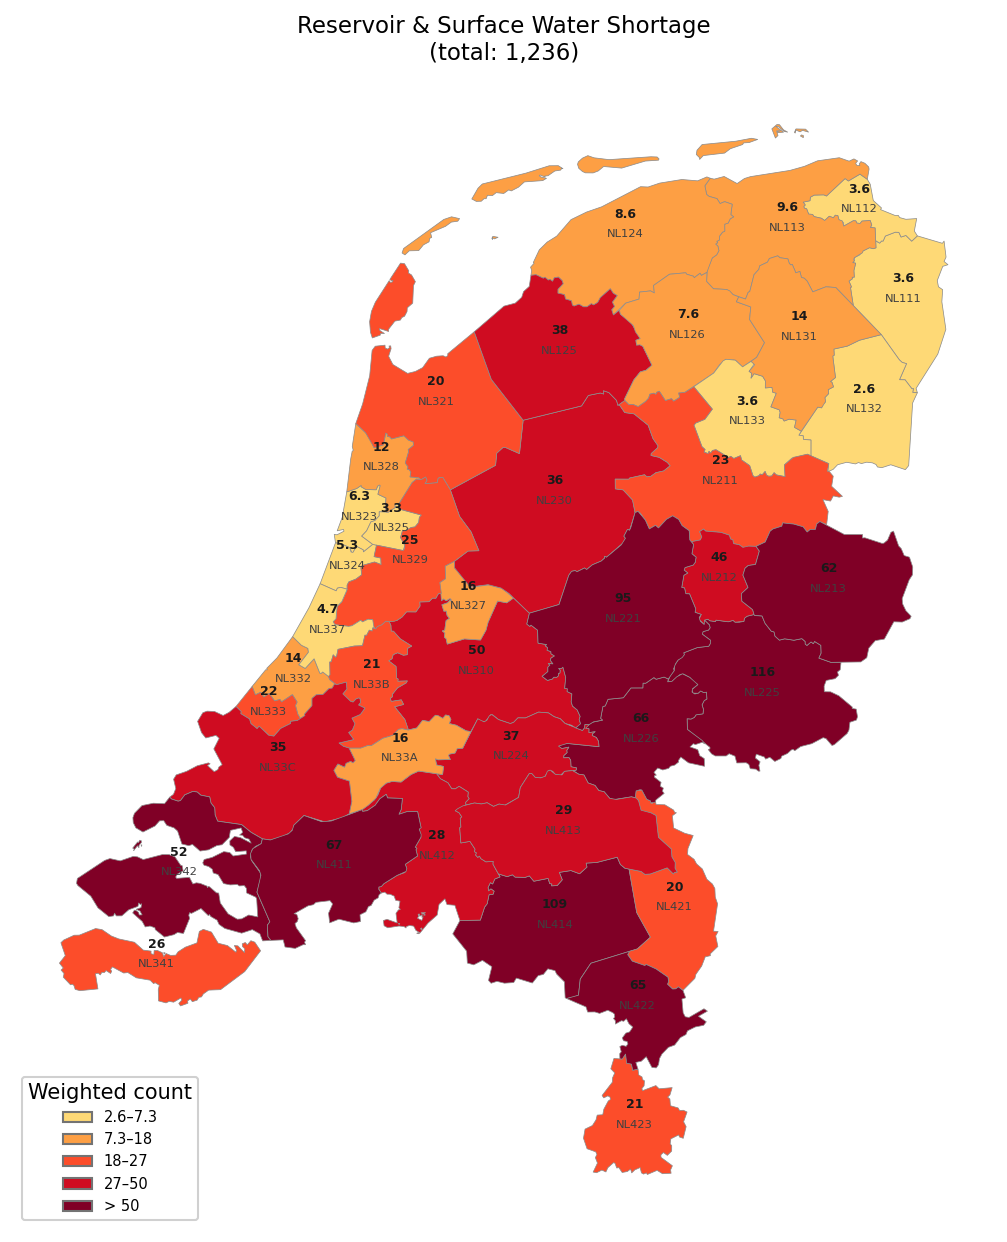
\includegraphics[width=\linewidth]{figures/Appendix C images/choropleth_reservoir_surface_water_shortage.png}
    \caption{Reservoir and surface water shortage}
\end{subfigure}
\hfill
\begin{subfigure}{0.32\textwidth}
    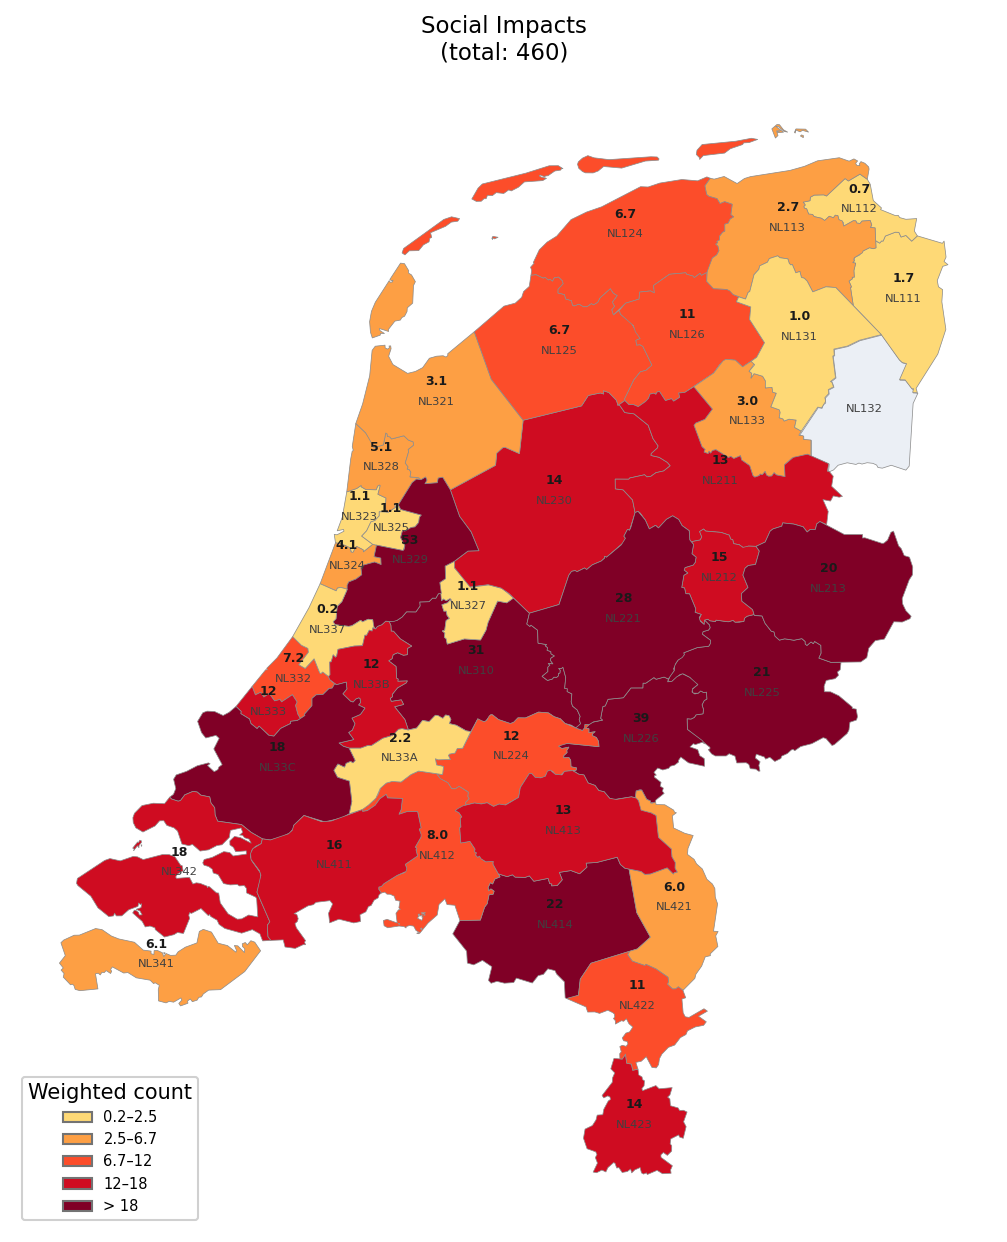
\includegraphics[width=\linewidth]{figures/Appendix C images/choropleth_social_impacts.png}
    \caption{Social impacts}
\end{subfigure}
\hfill
\begin{subfigure}{0.32\textwidth}
    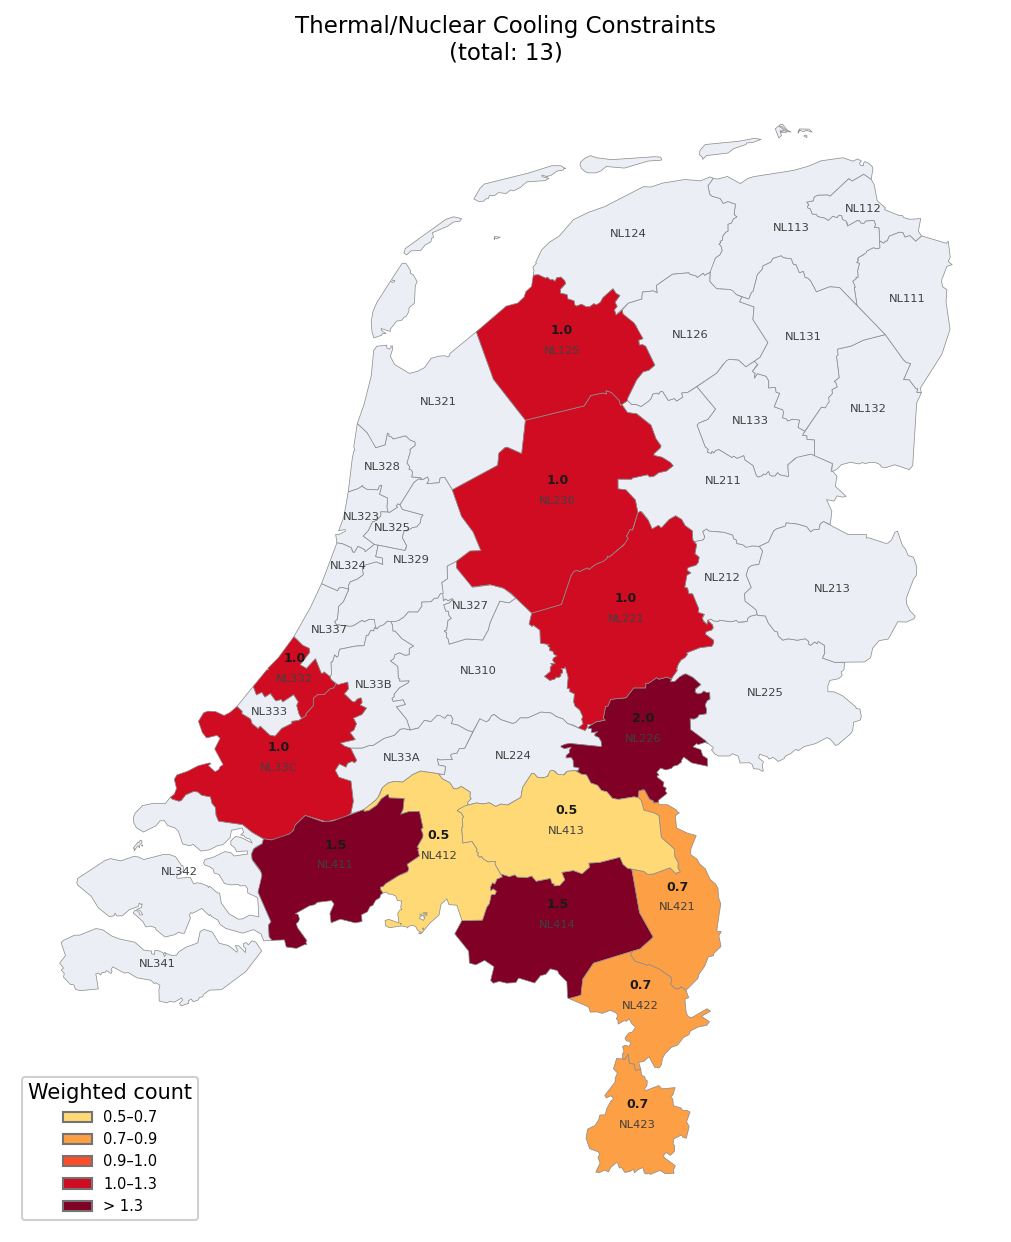
\includegraphics[width=\linewidth]{figures/Appendix C images/choropleth_thermal_nuclear_cooling_constraints.png}
    \caption{Thermal and nuclear cooling constraints}
\end{subfigure}

\vspace{0.5cm}

% Row 3
\begin{subfigure}{0.32\textwidth}
    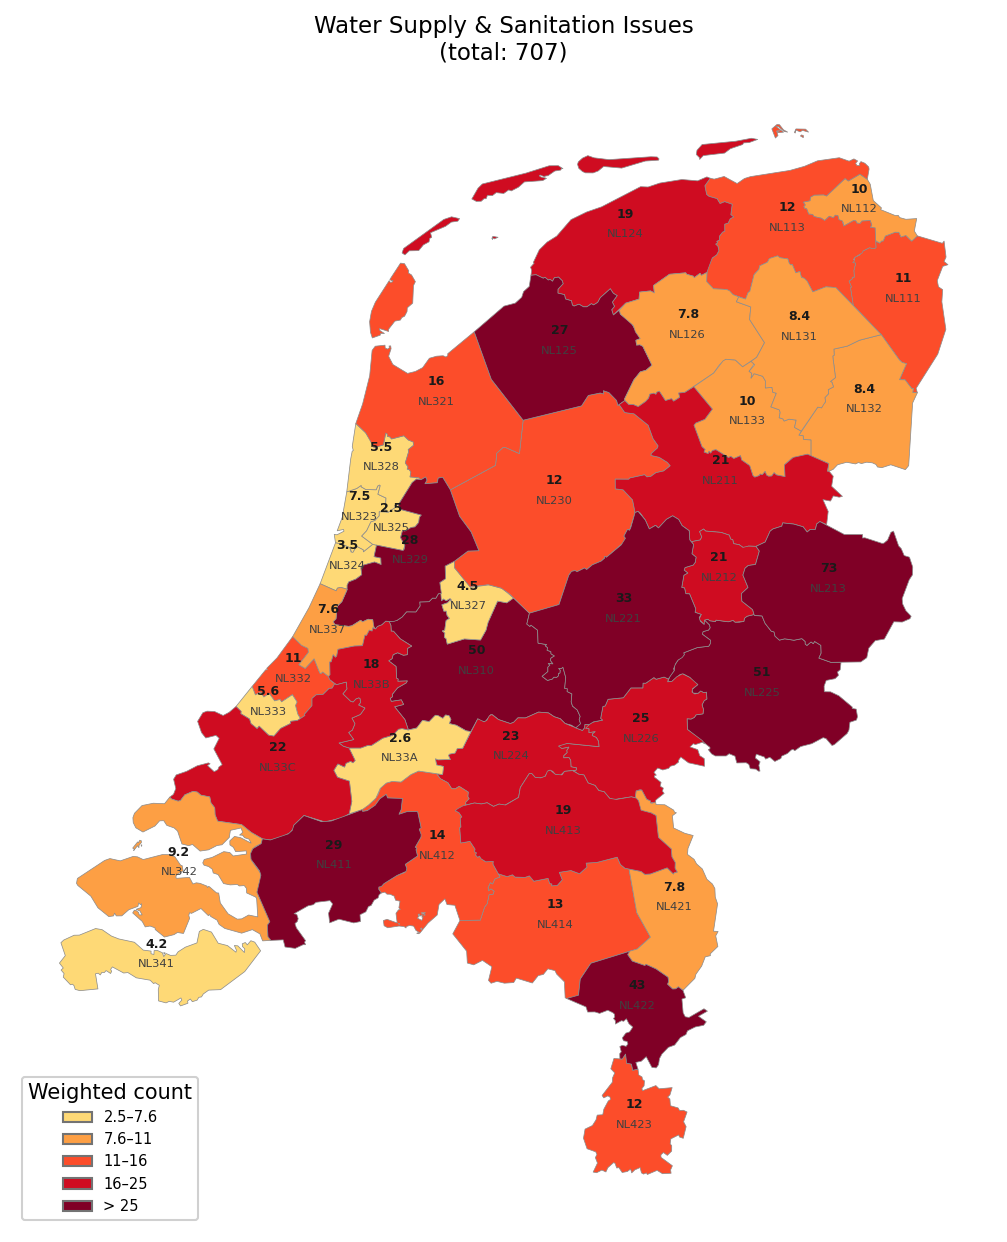
\includegraphics[width=\linewidth]{figures/Appendix C images/choropleth_water_supply_sanitation_issues.png}
    \caption{Water supply and sanitation issues}
\end{subfigure}
\hfill
\begin{subfigure}{0.32\textwidth}
    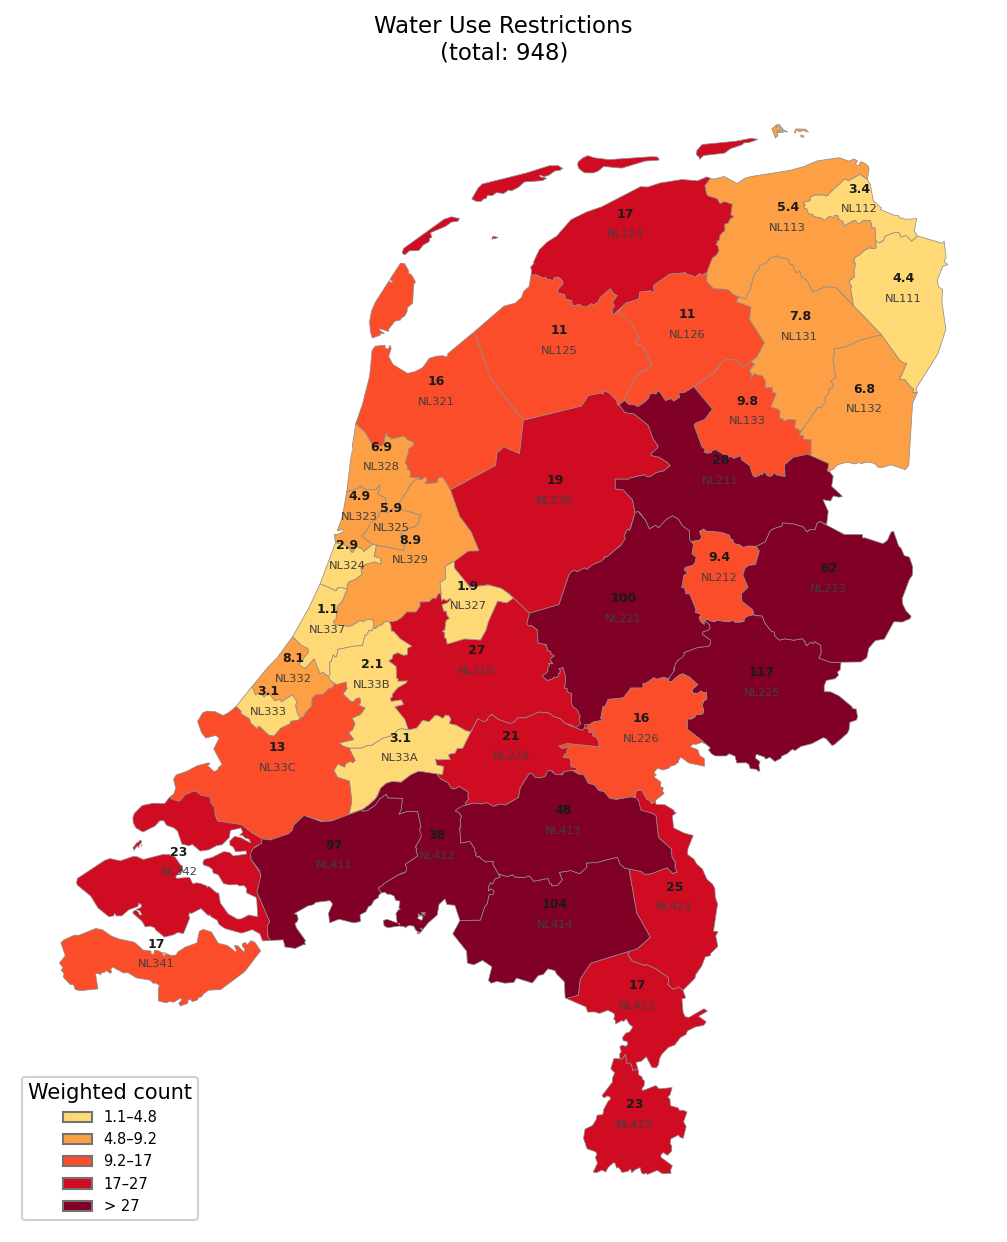
\includegraphics[width=\linewidth]{figures/Appendix C images/choropleth_water_use_restrictions.png}
    \caption{Water use restrictions}
\end{subfigure}
\hfill
\begin{subfigure}{0.32\textwidth}
    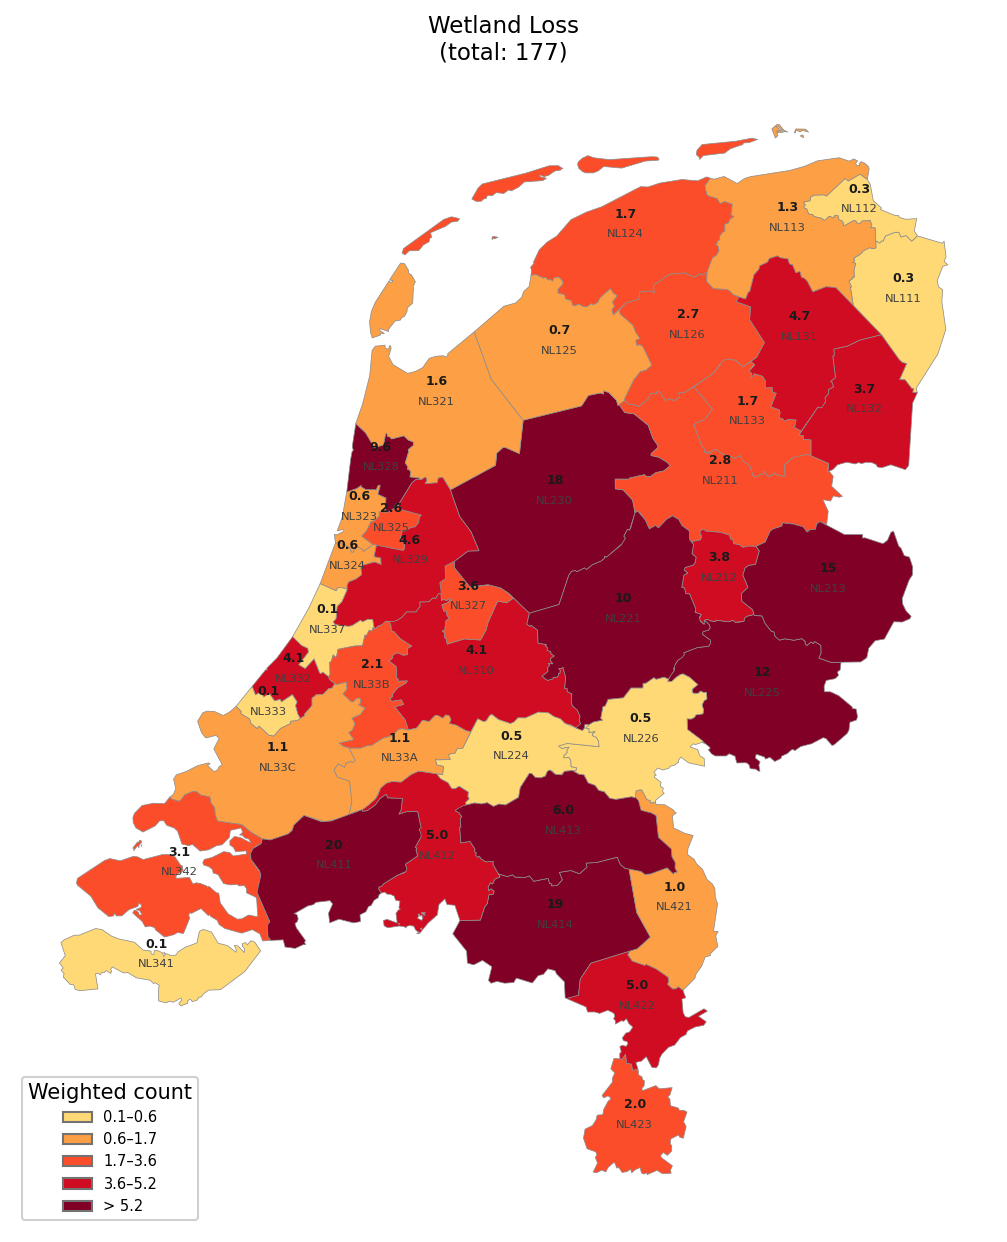
\includegraphics[width=\linewidth]{figures/Appendix C images/choropleth_wetland_loss.png}
    \caption{Wetland loss}
\end{subfigure}

\caption{Spatial distribution of drought impacts (Part 2).}
\label{fig:appendix_choropleths_2}
\end{figure}


\begin{figure}[p]
\centering

\begin{subfigure}{0.32\textwidth}
    \centering
    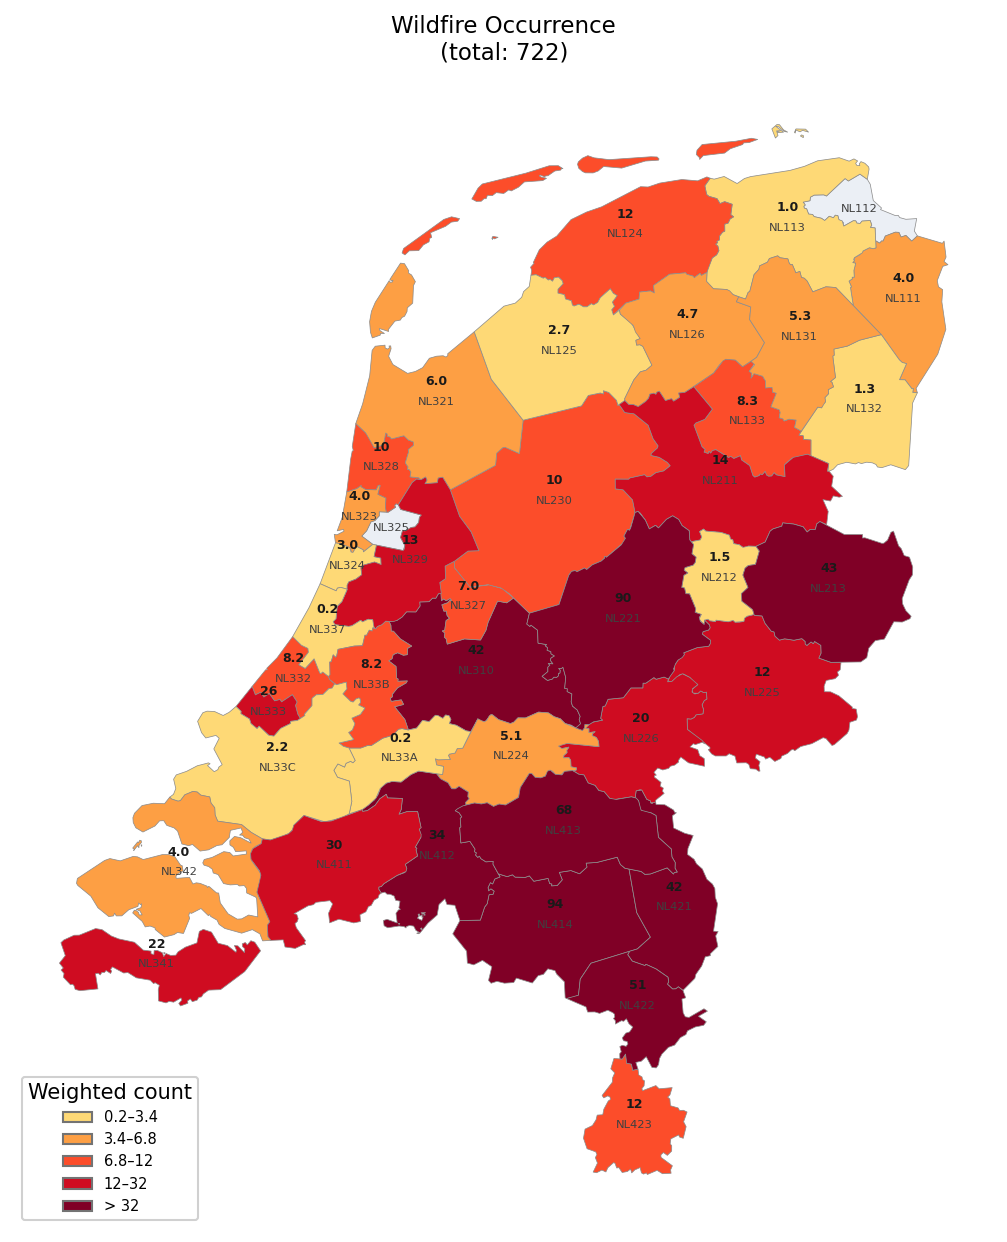
\includegraphics[width=\linewidth]{figures/Appendix C images/choropleth_wildfire_occurrence.png}
    \caption{Wildfire occurrence}
\end{subfigure}
\hfill
\begin{subfigure}{0.32\textwidth}
    \centering
    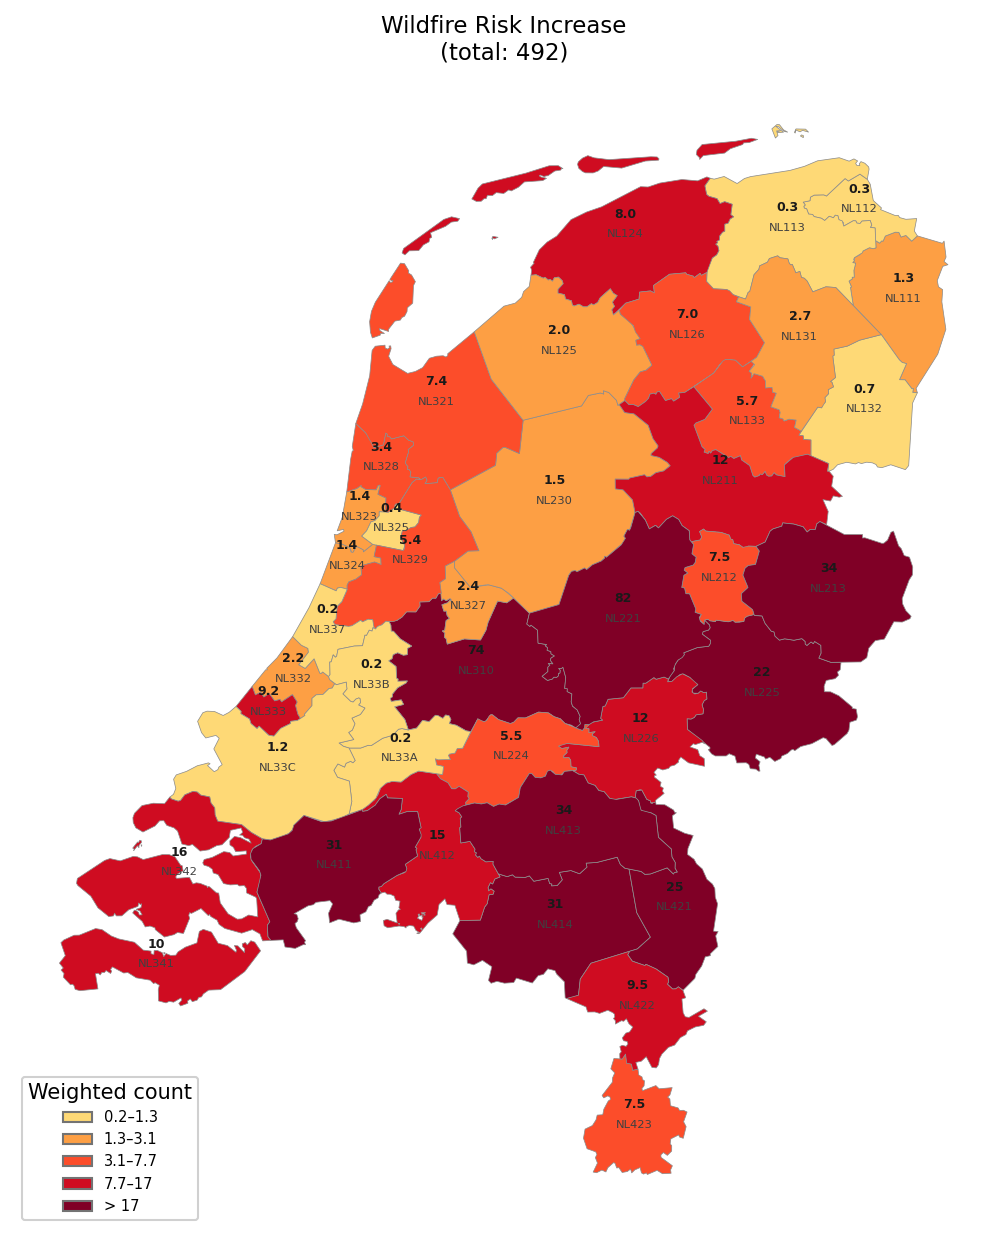
\includegraphics[width=\linewidth]{figures/Appendix C images/choropleth_wildfire_risk_increase.png}
    \caption{Wildfire risk increase}
\end{subfigure}

\caption{Spatial distribution of wildfire-related drought impacts (Part 3).}
\label{fig:appendix_choropleths_3}
\end{figure}

%add how much it costed and why it went wrong lopl

\backmatter
\bibliographystyle{alpha}
\bibliography{references,IBF_references, Location_extraction, LLMN_references}

\end{document}